\documentclass{thesisclass}
% Based on thesisclass.cls of Timo Rohrberg, 2009
% ----------------------------------------------------------------
% Thesis - Main document
% ----------------------------------------------------------------


%% -------------------------------
%% |  Information for PDF file   |
%% -------------------------------
\hypersetup{
 pdfauthor={Not set},
 pdftitle={Not set},
 pdfsubject={Not set},
 pdfkeywords={Not set}
}


%% ---------------------------------
%% | Information about the thesis  |
%% ---------------------------------

\newcommand{\myname}{Benjamin Tenke}
\newcommand{\mytitle}{Entwicklung eines Systems zur Bewertung von Beziehungen zwischen Personen aus einer CRM-Lösung}
\newcommand{\myinstitute}{}

\newcommand{\reviewerone}{Prof. Dr. Thomas Morgenstern}
\newcommand{\reviewertwo}{Prof. Dr. Andreas Schmidt}
\newcommand{\advisor}{Michal Dvorak}
\newcommand{\advisortwo}{Ludwig Neer}

\newcommand{\timestart}{28. Dezember 2013}
\newcommand{\timeend}{28. Dezember 2013}
\newcommand{\submissiontime}{DD. MM. 20XX}

%% ---------------------------------
%% | ToDo Marker - only for draft! |
%% ---------------------------------
% Remove this section for final version!
\setlength{\marginparwidth}{20mm}

\newcommand{\margtodo}
{\marginpar{\textbf{\textcolor{red}{ToDo}}}{}}

\newcommand{\todo}[1]
{{\textbf{\textcolor{red}{(\margtodo{}#1)}}}{}}


%% --------------------------------
%% | Old Marker - only for draft! |
%% --------------------------------
% Remove this section for final version!
\newenvironment{deprecated}
{\begin{color}{gray}}
{\end{color}}


%% --------------------------------
%% | Settings for word separation |
%% --------------------------------
% Help for separation:
% In german package the following hints are additionally available:
% "- = Additional separation
% "| = Suppress ligation and possible separation (e.g. Schaf"|fell)
% "~ = Hyphenation without separation (e.g. bergauf und "~ab)
% "= = Hyphenation with separation before and after
% "" = Separation without a hyphenation (e.g. und/""oder)

% Describe separation hints here:
\hyphenation{
% Pro-to-koll-in-stan-zen
% Ma-na-ge-ment  Netz-werk-ele-men-ten
% Netz-werk Netz-werk-re-ser-vie-rung
% Netz-werk-adap-ter Fein-ju-stier-ung
% Da-ten-strom-spe-zi-fi-ka-tion Pa-ket-rumpf
% Kon-troll-in-stanz
}


%% ------------------------
%% |    Including files   |
%% ------------------------
% Only files listed here will be included!
% Userful command for partially translating the document (for bug-fixing e.g.)
\includeonly{%
titlepage,
abstract,
declaration,
Chapter_Einfuehrung,
Chapter_Grundlagen,
Chapter_Analyse,
Analyse_ausgewaehlter_Datenbanken,
Chapter_Entwurf,
Chapter_Umsetzung,
Chapter_Zusammenfassung,
appendix
}

\lstset{
  frame=single, 
  keepspaces=true,
  captionpos=b,
  numbers=left,
  stepnumber=1,    
  firstnumber=1,
  tabsize=2,
  numberfirstline=true
}

%%%%%%%%%%%%%%%%%%%%%%%%%%%%%%%%%
%% Here, main documents begins %%
%%%%%%%%%%%%%%%%%%%%%%%%%%%%%%%%%
\begin{document}

\frontmatter
\pagenumbering{roman}
%% titlepage.tex
%%

% coordinates for the bg shape on the titlepage
\newcommand{\diameter}{20}
\newcommand{\xone}{-15}
\newcommand{\xtwo}{160}
\newcommand{\yone}{15}
\newcommand{\ytwo}{-253}

\begin{titlepage}
% bg shape
\begin{tikzpicture}[overlay]
\draw[color=gray]  
 		 (\xone mm, \yone mm)
  -- (\xtwo mm, \yone mm)
 arc (90:0:\diameter pt) 
  -- (\xtwo mm + \diameter pt , \ytwo mm) 
	-- (\xone mm + \diameter pt , \ytwo mm)
 arc (270:180:\diameter pt)
	-- (\xone mm, \yone mm);
\end{tikzpicture}
	\begin{textblock}{10}[0,0](4,2.5)
		
\includegraphics[width=.5\textwidth]{logos/HSKALogo_RGB.pdf}
	\end{textblock}
	\changefont{phv}{m}{n}	% helvetica	
	\vspace*{3.5cm}
	\begin{center}
		\Huge{\mytitle}
		\vspace*{1.3cm}\\
		\Large{
			\iflanguage{english}{Diploma Thesis of}			
												  {Bachelor-Thesis\\von}
		}\\
		\vspace*{1cm}
		\huge{\myname}\\
		\vspace*{1cm}
		\Large{
			\iflanguage{english}{At the Department of Informatics}			
													{An der Fakult\"at f\"ur Informatik und Wirtschaftsinformatik}
			\\
			\myinstitute
		
		
		}
		\Large{
			\iflanguage{english}{At the Department of Informatics}			
													{Fachgebiet Wirtschaftsinformatik}
			\\
			\myinstitute
		
		
		}
	\end{center}
	\vspace*{1cm}
\Large{
\begin{center}
\begin{tabular}[ht]{l c l}
  % Gutachter sind die Professoren, die die Arbeit bewerten. 
      \iflanguage{english}{Second reviewer}{Arbeitsplatz}: & \hfill & CAS Software AG, Karlsruhe\\
  \iflanguage{english}{Reviewer}{Erstgutachter}: & \hfill  & \reviewerone\\
  \iflanguage{english}{Second reviewer}{Zweitgutachter}: & \hfill  & \reviewertwo\\
 \iflanguage{english}{Second reviewer}{Abgabetermin}: & \hfill & 28.02.2014\\
  % Der zweite betreuende Mitarbeiter kann weggelassen werden. 
\end{tabular}
\end{center}
}


\vspace{0.5cm}
\begin{flushleft}

\large{\iflanguage{english}{Duration:}{Karlsruhe, den } \timestart \hspace*{0.25cm}}
\end{flushleft}

\vspace{1cm}
\begin{flushleft}

\large{\iflanguage{english}{Duration:}{Vorsitzender des \\ Prüfungsausschusses} \hspace*{0.25cm}}
\end{flushleft}


\begin{textblock}{10}[0,0](4,16.8)
\tiny{ 
	\iflanguage{english}
		{KIT -- University of the State of Baden-Wuerttemberg and National Research Center of the Helmholtz Association}
		{}
}
\end{textblock}

\begin{textblock}{10}[0,0](14,16.75)
\large{
	\textbf{} 
}
\end{textblock}

\end{titlepage}

\vspace*{36\baselineskip}
\hbox to \textwidth{\hrulefill}
\par
\iflanguage{english}{I declare that I have developed and written the enclosed thesis completely by myself, and have not used sources or means without declaration in the text.}{Ich versichere wahrheitsgem\"a\ss, die Arbeit selbstst\"andig angefertigt, alle benutzten Hilfsmittel vollst\"andig und genau angegeben und alles kenntlich gemacht zu haben, was aus Arbeiten anderer unver\"andert oder mit Ab\"anderungen entnommen wurde.}

\textbf{PLACE, DATE}
\vspace{1.5cm}

\dotfill\hspace*{8.0cm}\\
\hspace*{2cm}(\textbf{YOUR NAME}) %center name with hspace

\thispagestyle{empty}

\chapter*{\centering Zusammenfassung}

Die heutige Wirtschaft ist durch eine hohe Komplexität und Veränderungen interner und externer Rahmenbedingungen gekennzeichnet. In Zuge dessen gewinnen analytische Informationssysteme immer mehr an Bedeutung. Sie dienen der Unterstützung von Führungskräften, indem sie Entscheidung unterstützende Informationen zur Verfügung stellen. Zur Bereitstellung solcher Informationen werden verschiedene Technologien, wie Online-Analytical-Processing (OLAP), Data Warehousing und Data Mining eingesetzt. Mittels der zuvor genannten Technologien werden heutzutage analytische Softwarelösungen für Unternehmen umgesetzt. Allerdings bieten Produkte aus diesem Bereich keine optimale Lösung für alle Probleme und Fragestellungen der Industrie. In vielen Unternehmen werden daher einzelne Bestandteile solcher Systeme basierend auf den vorliegenden Anforderungen selbst entwickelt.

Im Zuge dieser Arbeit wird basierend auf den Daten eines CRM-Systems eine solche Eigenentwicklung geplant und umgesetzt. Mithilfe dessen eine performante Bewertung von Beziehungen zwischen den Personen eines CRM-Systems realisiert werden soll. Dazu werden im Vorfeld Grundlagen über neue Entwicklungen im Datenbankumfeld, sowie Technologien die in CAS genesisWorld Verwendung finden vorgestellt. Vor der eigentlichen Planung des Systems, werden relevante Komponenten von CAS genesisWorld untersucht und Anforderungen an das neue System erhoben. Aufbauend auf den gewonnen Informationen  werden passenden Technologien ausgewählt, sowie Strukturen und Konzepte zur Umsetzung erarbeitet. Überdies wird der Prozess zur Extraktion und Transformation der Daten aus der alten in die neue Datenbank entworfen. Basierend auf den zuvor entworfenen Konzepten werden die Umsetzungen im Detail beschrieben. Die Ergebnisse werden im Anschluss anhand fachlicher und technischer Anforderungen bewertet.
\blankpage


%% -------------------
%% |   Directories   |
%% -------------------
\tableofcontents
\listoffigures
\listoftables

%% -----------------
%% |   Main part   |
%% -----------------
\mainmatter
\pagenumbering{arabic}
%% content.tex
%%

%% ==============
\chapter{Einführung}
%% ==============

...

%% ===========================
\section{Motivation}
%% ===========================

...

%% ===========================
\section{Zielsetzung}
%% ===========================

...

%% ===========================
\section{Gliederung der Arbeit}
%% ===========================

...
%% content.tex
%%

%% ===========================
\chapter{Grundlagen}
\label{ch:grundlagen}
%% ===========================

Das Kapitel Grundlagen geht zu Beginn auf den Begriff NoSQL ein und stellt  verschiedene NoSQL-Implementierungen vor. Dabei wird unter anderem auf grundlegende Begriffe aus dem NoSQL Umfeld eingegangen. Anschließend werden Eigenschaften und Unterscheidungsmerkmale von In-Memory-Datenbanenk behandelt. Abschließend soll ein Einblick in das Component Object Model (COM) gegeben werden. Dabei wird die allgemeine Funktionsweise dargelegt und wichtige Komponenten des Standards erläutert.

%% ===========================
\section{NoSQL - Eine Einführung}
\label{ch:grundlagen:sec:NoSQL}
%% ===========================

Der Terminus NoSQL bezeichnet Datenbanken die nicht dem Ansatz der relationalen Algebra folgen. Ihre Entstehung ist auf die schlechte horizontale Skalierbarkeit von relationalen Datenbanken zurückzuführen. Verfügbarkeit und Skalierbarkeit sind unter gewissen Umständen wichtiger als Atomarität und Konsistenz. Dieser Umstand führte neben der Entwicklung von NoSQL-Datenbanken zur Entstehung von Datenbanken die unter dem Terminus NewSQL zusammengefasst werden. Sie verfolgen einen anderen Ansatz als NoSQL-Datenbanken und werden im Rahmen dieser Arbeit nicht näher betrachtet, weshalb weiterhin auf \cite{NewSQL2011} verwiesen wird. Weiterhin lassen sich NoSQL-Datenbanken anhand ihres Datenmodells unterscheiden. Nach \cite{vaish2013getting} ist eine Klassifizierung in folgende Kategorien möglich:

%% ===========================
\subsection{Document Stores}
\label{ch:grundlagen:sec:NoSQL:DocumentStores}
%% ===========================

Document Stores koppeln komplexe Datenstrukturen (Dokumente) mit einem eindeutigen Schlüssel. Der Datenzugriff findet in der Regel über das HTTP-Protokoll mit REST-API oder über das Apache Thrift-Protokoll statt \cite{agarwal2007thrift}. In Document Stores gibt es außerdem kein Schema. Statt jeden Datensatz in einer Zeile bestehend aus Spalten zu speichern, werden sie in einem Dokument abgelegt. Diese können als eine Datei auf dem Dateisystem betrachtet werden. Solche Dokumente können alle möglichen Daten aufnehmen und müssen dabei keinem Schema folgen. Trotz der Schemafreiheit sind sie nicht frei von formellen Restriktionen. Die meisten der verfügbaren Datenbanken unter dieser Kategorie benutzen XML, JSON, BSON oder YAML. Document Stores eignen sich für den Einsatz von dynamischen Entitäten, die unregelmäßige Strukturen besitzen.

%% ===========================
\subsection{Extensible Record Store}
\label{ch:grundlagen:sec:NoSQL:ExtensibleRecordStore}
%% ===========================

Extensible Record Stores, auch Wide Column Stores genant, speichern Daten mehrerer Einträge in Spalten anstatt in Zeilen. Jeder Eintrag einer Spalte besteht aus einem Namen, den Daten und einem Zeitstempel.

In Extensible Record Stores werden sogenannte Spalten-Familien zur Gruppierung ähnlicher oder verwandter Inhalte verwendet. In Abbildung \ref{wide_column_store} ist eine solche Spalten-Familie zu sehen. Spalten-Familien besitzen keine logische Struktur und geben somit kein Schema vor. Weiterhin können sie Millionen von Spalten beinhalten. Verwandte Spalten werden in Spalten-Familien durch eine von der Anwendung bereitgestellte Reihe von Schlüsseln identifiziert. Weiterhin muss in einer Spalten-Familie nicht jede Zeile aus den gleichen Spalten bestehen.

\begin{figure}[htbp]
	\centering
  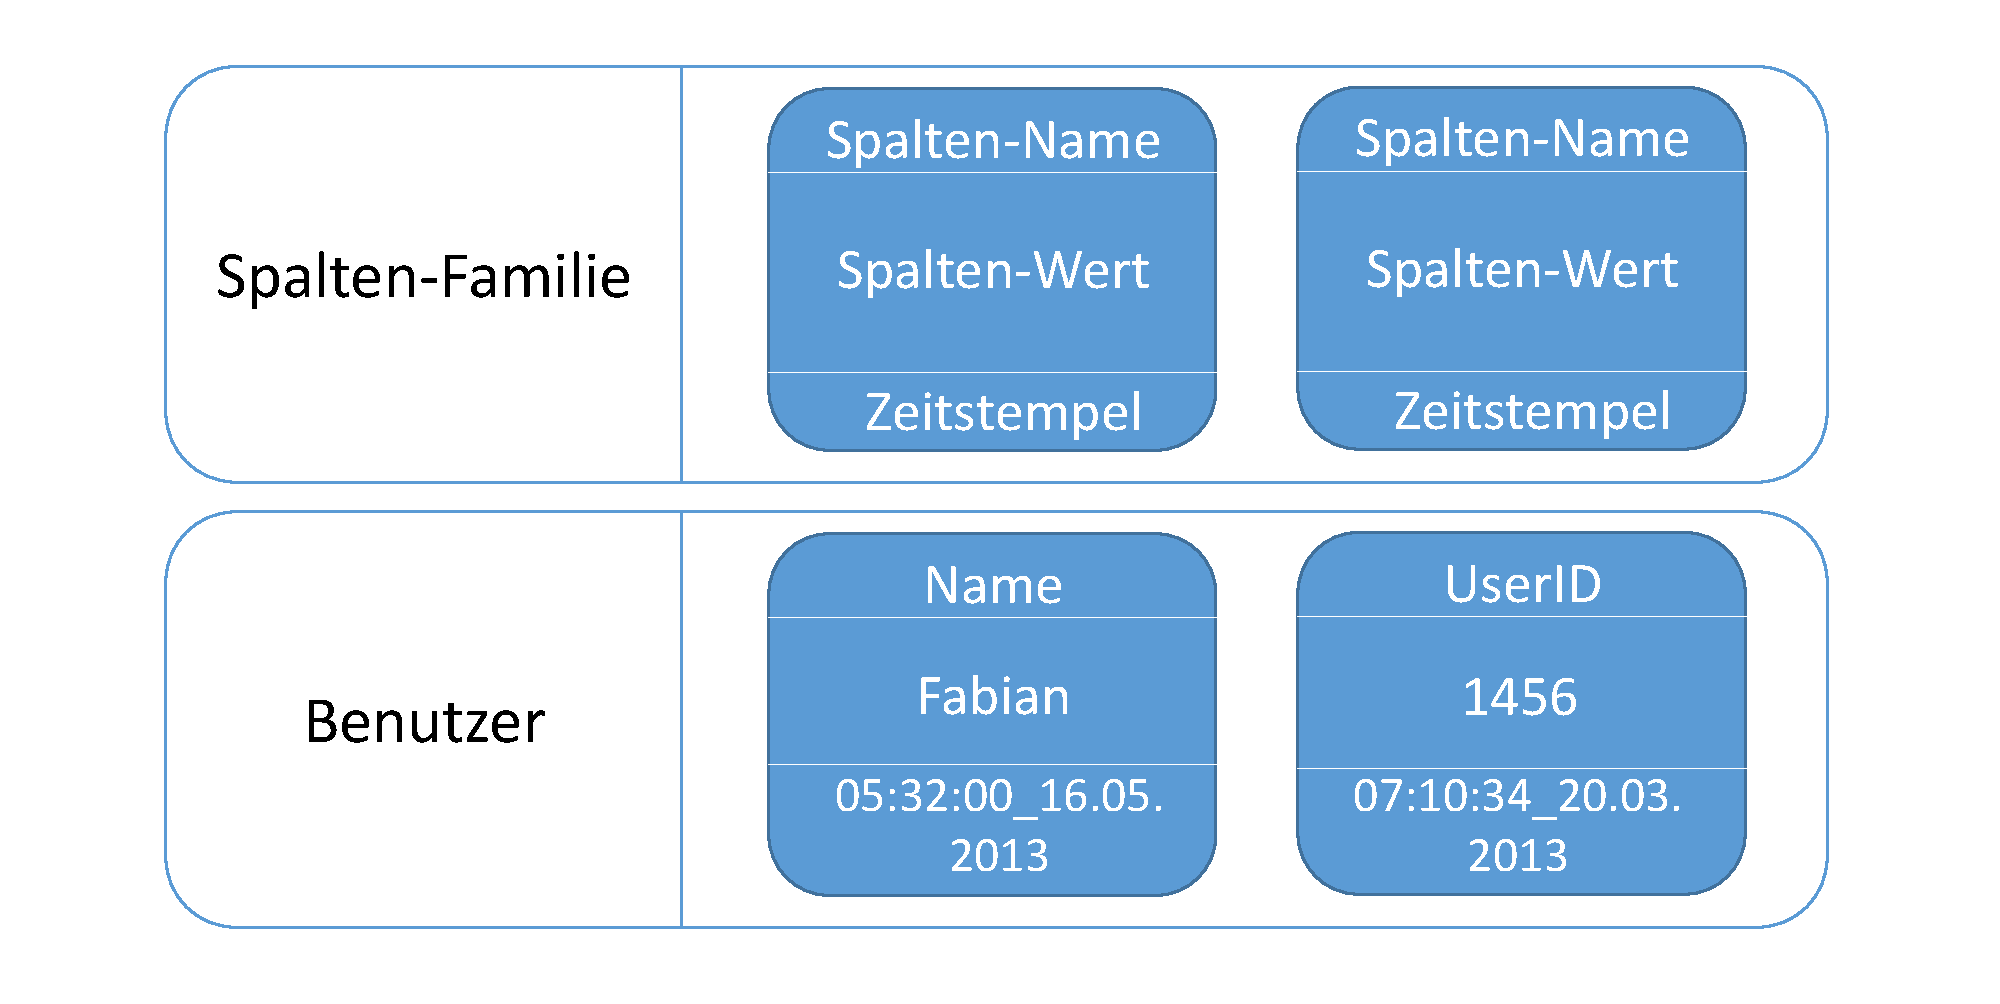
\includegraphics[width=0.8\textwidth, width=0.8\textwidth]{pics/wide_column_stores.pdf}
	\caption{Beispiel einer Spalten-Familie}
	\label{wide_column_store}
\end{figure}



%% ===========================
\subsection{Key-Value-Store}
\label{ch:grundlagen:sec:NoSQL:KeyValueStore}
%% ===========================

Grundsätzlich verwendet der Key-Value-Store eine einfache Form der Datenspeicherung. Ein bestimmter Schlüssel referenziert auf einen Wert, der eine willkürliche Zeichenkette sein kann. In einigen Umsetzungen können die Werte außer Strings auch Listen, Sets oder auch Hashes beinhalten. Der Zugriff auf die Werte erfolgt über einen eindeutigen Schlüssel, d.h. jeder Schlüssel repräsentiert ein eindeutig identifizierbares Objekt. Im Gegensatz zu relationalen Datenbanken haben Key-Value-Stores keine Kenntnis über das Datenmodell und sind daher schemafrei. Sie setzen sich zum Ziel skalierbar und fehlertolerant zu sein. Zu den Einsatzorten zählen Web-Applikationen mit vielen aber einfachen Daten.

%% ===========================
\subsection{Graphdatenbank}
\label{ch:grundlagen:sec:NoSQL:GraphDatenbanken}
%% ===========================

Eine Graphdatenbank verwendet die Graphentheorie zur Abbildung und Abfrage von Beziehungen \cite{SWB-386976589}. Im Grunde besteht eine solche Datenbank aus einer Menge von Knoten und Kanten. Jeder Knoten repräsentiert dabei eine Entität, wohingegen Kanten Beziehungen oder Verbindung zwischen zwei Knoten darstellen. Abbildung \ref{graph_database} verdeutlicht dies in einem Beispiel. Knoten definieren sich durch einen sogenannten "unique identifier", sowie durch die Anzahl abgehenden und/oder eingehenden Kanten und einer Menge von Attributen. Kanten werden wie Knoten definiert, nur dass diese, anstatt Kanten, einen Start- und End-Knoten besitzen. Graphdatenbanken eignen sich gut für die Analyse von Verbindungen, weshalb sie oft zur Datengewinnung im Social Media Umfeld genutzt werden.

\begin{figure}[htbp]
	\centering
  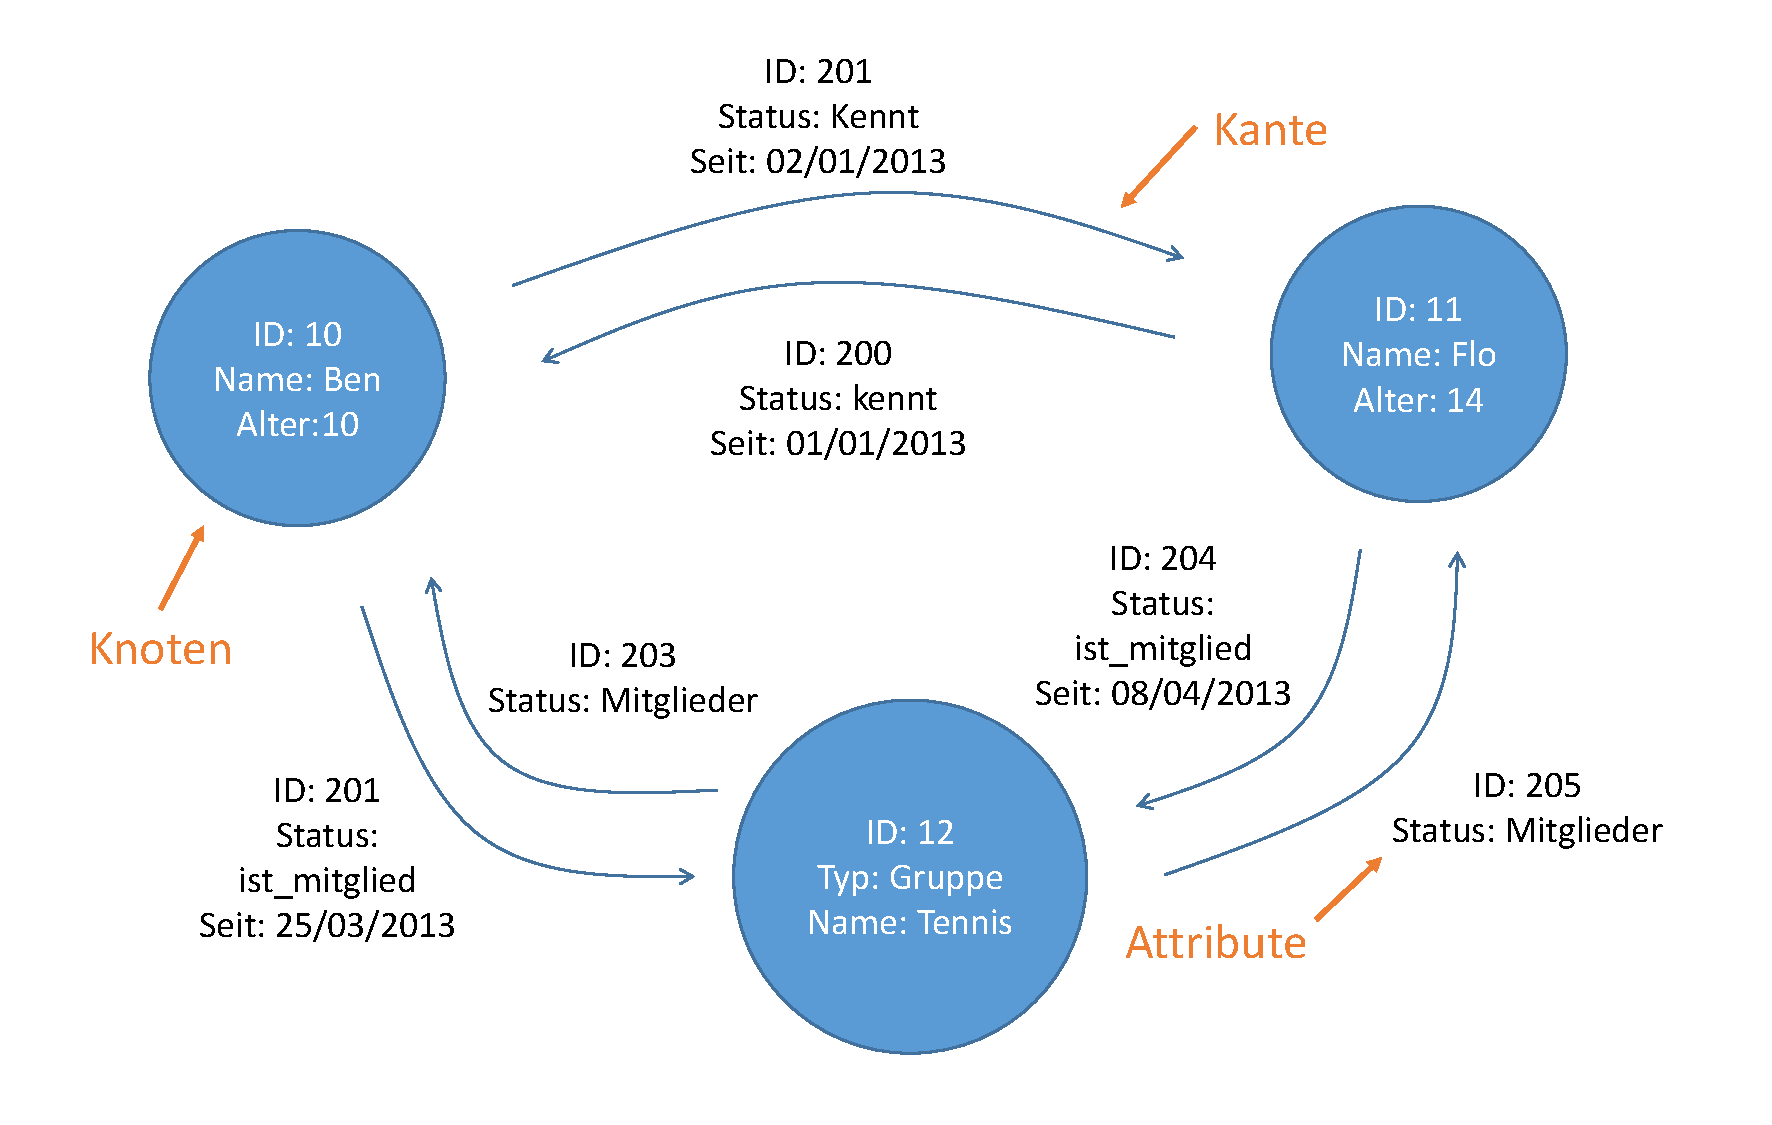
\includegraphics[width=1.0\textwidth, width=1.0\textwidth]{pics/graphdatabase.pdf}
	\caption{Objekte in einer Graphdatenbank}
	\label{graph_database}
\end{figure}

%% ===========================
\subsection{Theoretische Grundlagen}
\label{ch:grundlagen:sec:NoSQL:NoSQLBasics}
%% ===========================

Im Nachfolgenden werden die durch die NoSQL Bewegung geprägten Begriffe und Konzepte erläutert.

\paragraph{Replikation} Replikation im Falle von verteilten Datenbanken bedeutet, dass ein Datenelement auf mehr als einem Knoten (Computer) gespeichert ist. Dies ist sehr nützlich, um Leseleistungen der Datenbanken und deren Ausfallsicherheit zu erhöhen. Ermöglicht wird dies durch einen Load-Balancer, der Lesevorgänge über viele Maschinen verteilt.

\paragraph{Fragmentierung} Fragmentierung in der Datenbank bedeutet eine Verteilung des Datenbestandes auf verschiedene Fragmente. Diese können dann über viele Knoten verteilt werden. Die Datenpartitionierung kann beispielsweise mit einer konsistenten Hash-Funktion erfolgen, die auf dem Primärschlüssel der Datenelemente angewendet wird, um das zugehörige Fragment zu bestimmen.

\paragraph{Eventual-Consistency} Später in diesem Kapitel wird das CAP-Theorem eingeführt, welches besagt, dass verteilte Datenbanken entweder stark konsistent oder verfügbar sein können. Da die meisten NoSQL-Datenbanken Verfügbarkeit priorisieren, wird in diesen Datenbanken das Konzept Eventual-Consistency eingesetzt. Es stellt eine abgeschwächte Art der starken Konsistenz dar. Starke Konsistenz bedeutet, dass alle mit der Datenbank verbundenen Prozesse immer die gleiche Version der Daten sehen. Eventuelle Konsistenz ist schwächer und garantiert nicht, dass jeder Prozess die selbe Version sieht.

\paragraph{Multiversion Concurrency Control (MVCC)} MVCC ist eine effiziente Methode, mehrere Prozesse auf die selben Daten parallel zugreifen zu lassen, ohne eine Beschädigung der Daten und Deadlocks zu riskieren. Es ist eine Alternative zu den Lock-basierten Ansätzen, bei der jeder Prozess zuerst eine exklusive Sperre auf einem Datenelement anfordern muss, bevor er ihn lesen oder aktualisieren kann. Zu diesem Zweck werden intern verschiedene Versionen eines Objektes gehalten.

\paragraph{MapReduce} MapReduce ist ein von Google entwickeltes Programmiermodell für verteilte Berechnungen und wurde zuerst in einem Artikel von Dean und Ghemawat \cite{Dean:2008:MSD:1327452.1327492} beschrieben. Anwendungen, die mit dem MapReduce-Framework geschrieben werden, können automatisch auf mehreren Computern verteilt werden, ohne dass der Entwickler einen benutzerdefinierten Code für die Synchronisation und Parallelisierung schreiben muss. MapReduce wird in Fällen verwendet in denen einzelne Maschinen zu lange bräuchten um die gegebene Aufgabe zu bewältigen. 

\paragraph{Vektoruhren}
Vektoruhren  basieren auf der Arbeit von Lamport \cite{Lamport:1978:TCO:359545.359563} und werden von vielen Datenbanken verwendet, um festzustellen, ob ein Datenelement durch konkurrierende Prozesse verändert wurde. Jedes Datenelement besitzt eine Vektoruhr, welche aus Tupeln mit verschiedenen Zeitpunkten besteht. Jeder Zeitpunkt stellt einen Prozess dar, der eine Modifikation an dem Datenelement vorgenommen hat. Jede Uhr beginnt bei Null und wird durch seinen Prozess bei jedem Schreibvorgang erhöht. Um den eigenen Wert der Uhr zu erhöhen, verwendet der Schreibprozess das Maximum aller Werte der Uhren im Vektor und erhöht sie um eins. Wenn zwei Versionen eines Elements zusammengeführt werden, können die Vektoruhren benutzt werden, um Konflikte zu erkennen. Wenn mehr als ein Wert einer Uhr differenziert, muss ein Konflikt vorhanden sein. Wenn es keinen Konflikt gibt, kann die aktuelle Version durch den Vergleich der Maxima der Uhren ermittelt werden.

\paragraph{Das CAP-Theorem} Das CAP-Theorem wurde von Brewer erstmals in einem Symposium \cite{cap2010} über den Trade-Off in verteilten Systemen eingeführt und wurde später von Gilbert und Lynch \cite{Gilbert:2002:BCF:564585.564601} formalisiert. Es besagt, dass in einem verteilten Datenspeichersystem nur zwei Merkmale aus Verfügbarkeit, Konsistenz und  Partitionstoleranz garantiert werden können. Verfügbarkeit bedeutet in diesem Fall, dass die Clients in einem bestimmten Zeitraum immer Daten lesen und schreiben können. Eine partitionierte, verteilte Datenbank ist fehlertolerant gegenüber temporären Verbindungsproblemen und arbeitet auch bei Verlust von Nachrichten, einzelner Netzknoten oder Partition des Netzes weiter. Ein System das tolerant partitioniert ist, kann nur eine starke Konsistenz durch Verminderungen in seiner Verfügbarkeit erreichen. Grund dafür ist, dass es zuerst sicherstellen muss, ob jeder Schreibvorgang abgeschlossen wurde, bevor er eine Replikation durchführen kann. Allerdings kann es vorkommen, dass dies in einer verteilten Umgebung nicht möglich ist. Ursachen dafür können Verbindungsfehler oder andern temporäre Hardwareprobleme sein. Konsistenz bedeutet im Falle des CAP-Theorems, dass alle Knoten zur selben Zeit dieselben Daten sehen. 

%% ===========================
\section{In-Memory-Datenbanken}
\label{ch:grundlagen:sec:InMemoryDatenbanken}
%% ===========================

Eine In-Memory-Datenbank (IMDB) ist ein Datenbankmanagementsystem, das in erster Linie den Hauptspeicher als Medium für die Datenablage verwendet. Eine IMDB wird auch als Main-Memory-Database (MMDB) oder Real-Time-Database (RTDB) bezeichnet. IMDBs sind schneller als die auf Festplatten zugreifenden Datenbanken, da der Hauptspeicher wesentlich niedrigere Zugriffszeiten aufweist. Außerdem führen sie weniger CPU-Befehle beim Lesen und Schreiben aus und ihre internen Optimierungsalgorithmen sind viel einfacher gestaltet. Einsatz finden sie vor allem in Anwendungen in denen kurze Reaktionszeiten von entscheidender Bedeutung sind. Mehrkernprozessoren, 64-bit-Architekturen und gesunkene RAM-Preise stellen die treibenden Faktoren in der Entwicklung solcher Systeme dar \cite{SWB-381840476}.

Die hohe Performance dieser Systeme resultiert nicht nur durch die Datenhaltung im Hauptspeicher. Vielmehr müssen bisherige Konzepte im Datenbankentwurf neu überdacht werden. Beispielsweise besitzen IMDB, die den relationalen Ansatz verfolgen, geänderte Abfrageoptimierer. In herkömmlichen RDBMS sind Lese- und Schreiboperationen eine der wichtigsten Faktoren zur Bestimmung des optimalen Abfrageplans. In IMDB spielen sie allerdings eine stark untergeordnete Rolle. Im Gegenzug nimmt die Reduktion von CPU-Zyklen einen höheren Stellenwert ein.

In herkömmlichen Datenbanken ist der Speicherverbrauch kein relevanter Faktor. In IMDB hingegen ist der Einsatz von speicherplatzsparenden Maßnahmen eine Notwendigkeit. Dictionary Encoding, Run-Length Encoding oder Cluster Encoding sind nur einige Techniken zur Reduktion des Speicherplatzverbrauches. Solche Techniken bieten sich vor allem in spaltenorientierten Systemen aufgrund der eher geringeren Entropie innerhalb der Spalten an \cite{Abadi:2006:ICE:1142473.1142548}. Neben den Optimierungsansätzen in der Datenhaltung können Regeln formuliert werden, um nicht mehr verwendete Daten zu erkennen. Dabei kann z.B. zwischen aktiven Daten (Daten von nicht abgeschlossenen Geschäftsprozessen) und passiven Daten (Daten von abgeschlossenen Geschäftsprozessen) unterschieden werden \cite{10.1109/ICDE.2013.6544811}. Wenn ein Geschäftsprozess in sich abgeschlossen ist, werden die Daten nur noch aus Datenvorhaltungsgründen aufbewahrt. Die zur Datenaufbewahrung benötigte Hauptspeicherkapazität kann durch solche Regeln stark reduziert werden.

In traditionellen Datenbanken stellt das Wiederherstellen aufgrund des nicht flüchtigen Speichers kein Problem dar. IMDB müssen dagegen für den Fall eines Systemausfalls Snapshot-Dateien anlegen. Diese werden zur Wiederherstellung des Datenbestandes benötigt. Snapshots sind Abbilder des aktuellen Datenbestandes. Um Rücksicht auf die Performance zu nehmen, werden die Snapshots entweder in Intervallen oder zu festgelegten Ereignissen erzeugt. Damit die Veränderungen an Daten zwischen Snapshots nicht verloren gehen, werden sie in Log Dateien zwischengespeichert. Zusammen mit den Snapshots bilden sie die Grundlage für die Datenwiederherstellung. 

An dieser Stelle endet der Abschnitt über Datenbanken. Im Folgenden wird auf das Component Object Model eingegangen.

%% ===========================
\section{Component Object Model}
\label{ch:grundlagen:sec:ComponentObjectModel}
%% ===========================

Das Component Object Model (COM) ist ein binärer Schnittstellenstandard für Software-Komponenten, der von Microsoft im Jahr 1993 eingeführt wurde \cite{SWB-088582566}. Es wird verwendet um Interprozesskommunikation und dynamische Objekterstellung in einer Vielzahl von Programmiersprachen zu ermöglichen. Um zu verstehen was COM ist (und damit alle COM-basierten Technologien), muss einem klar sein, dass es sich nicht um eine objektorientierte Sprache, sondern um einen Standard zur Beschreibung von Objektmodellen handelt. Er definiert keine Sprache, Struktur oder Implementierungsdetails. Die jeweilige Umsetzung wird dem Programmierer überlassen. Es spezifiziert lediglich ein Objektmodell und die Anforderungen an die Kommunikationen zwischen COM-Objekten und anderen Objekten. Es spielt dabei keine Rolle, ob Objekte sich im gleichen oder in unterschiedlichen Prozessen befinden. Sie können sogar auf unterschiedlichen Rechnern laufen. Die Implementierung in verschiedenen Sprachen ist durch das Überführen der Kommunikation in binären Maschinencode möglich. Das führt dazu, dass COM des öfteren als binärer Standard referenziert wird.

COM bietet die Möglichkeit auf viele Windows-Funktionen direkt zuzugreifen. Des weiteren ist COM die Basis für die OLE–Automation\footnote{OLE ist ein dynamisches Datenaustauschverfahren zur dynamischen Verknüpfung von Objekten auf der Desktop-Ebene. Dadurch können Daten von OLE-fähigen Anwendungen untereinander verknüpft werden}(Object Linking and Embedding) und ActiveX\footnote{ActiveX bezeichnet ein Softwarekomponenten-Modell. Es ermöglicht den Zugriff auf Datenbanken sowie weiteren Anwendungen und Programmierungen. Im Internet-Explorer beispielsweise wird mithilfe von AktiveX der MediaPlayer zum öffnen von Multimedia-Dateien aufgerufen}. Die Verwendung des COM-Standards bietet folgende Vorteile:

\begin{itemize}
\item Sprachunabhängigkeit
\item Versionsunabhängigkeit
\item Plattformunabhängigkeit
\item Objektorientierung
\item Ortsunabhängigkeit
\item Automatisierung
\end{itemize} 

%% ===========================
\subsection{Architektur}
\label{ch:grundlagen:sec:ComponentObjectModel:subsec:Architektur}
%% ===========================

Wie in Abbildung \ref{GL_COM} zu sehen, erzeugt ein COM-Client eine COM-Komponente in einem so genannten COM-Server und nutzt die Funktionalität des Objektes über COM-Schnittstellen. 

\begin{figure}[htbp]
	\centering
  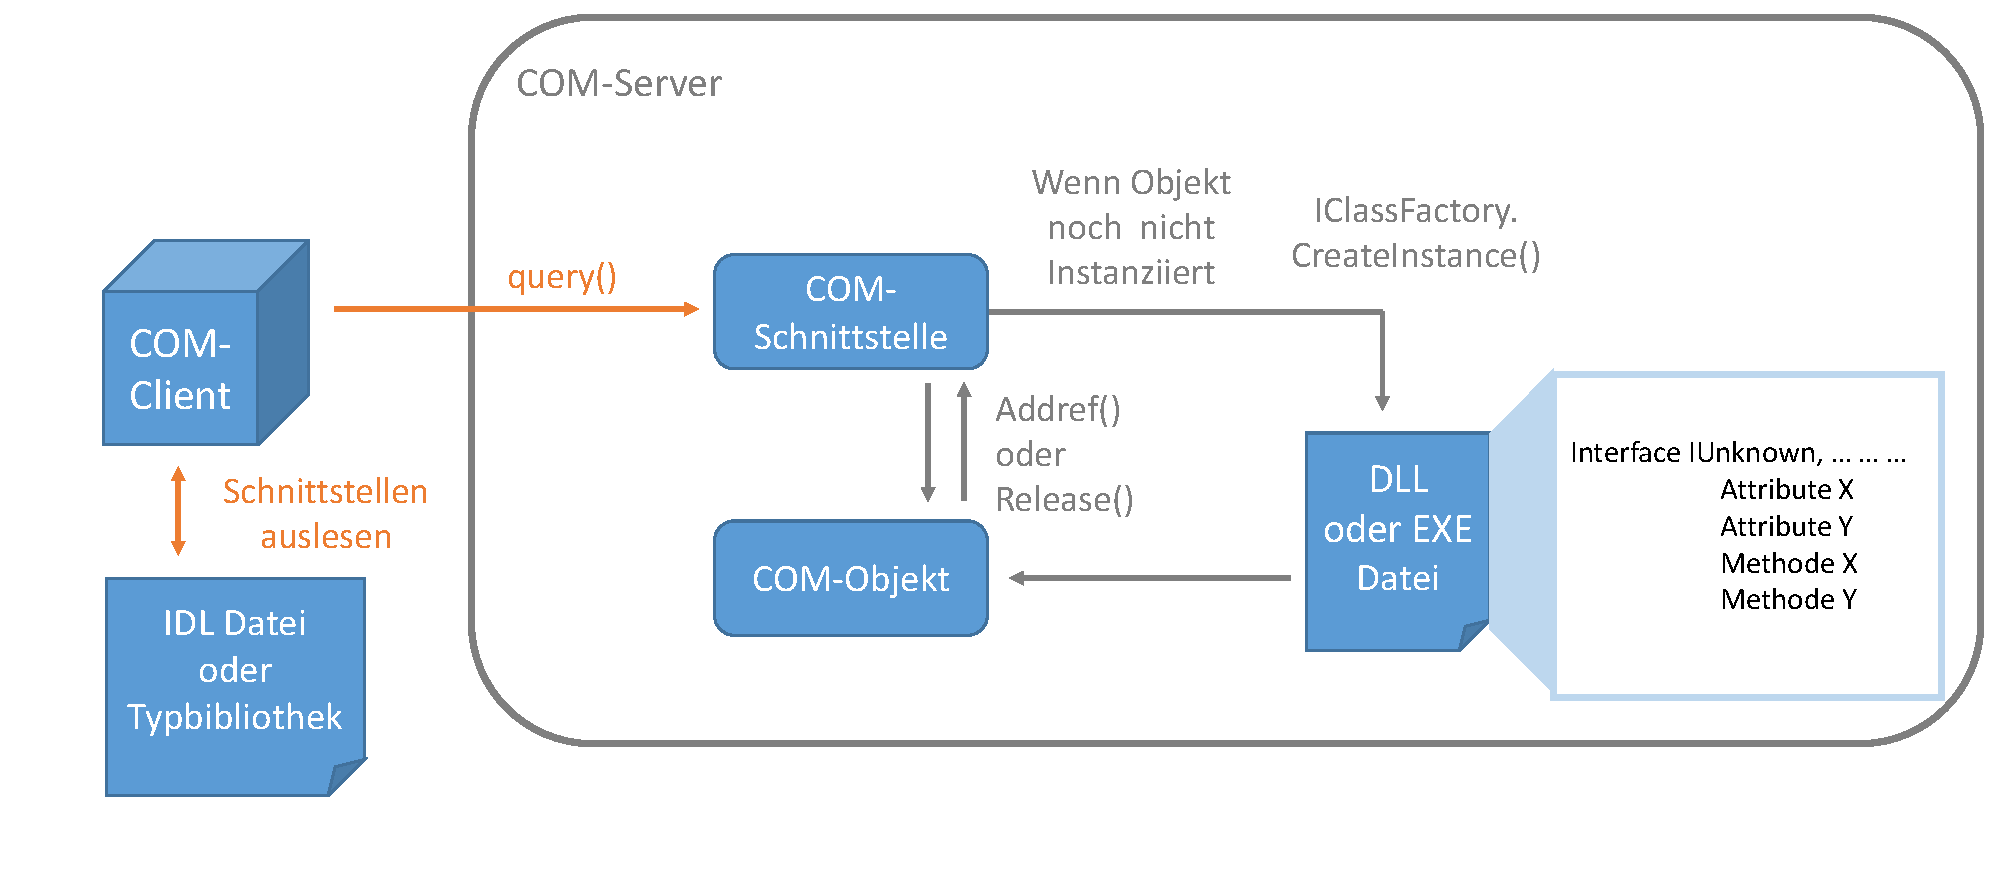
\includegraphics[width=1.0\textwidth, width=1.0\textwidth]{pics/Grundlagen_com.pdf}
	\caption{Das Konzept von COM}
	\label{GL_COM}
\end{figure} 

%% ===========================
\subsection{COM-Client}
\label{ch:grundlagen:sec:ComponentObjectModel:subsec:COMClient}
%% ===========================

Der COM-Client stellt den Benutzer einer COM-Komponente dar. Die Nutzung der COM-Komponenten erfolgt über sogenannte Interfaces. Interfaces liegen in Form von Beschreibungen in der Interface Definition Language (IDL) vor. Einem Client steht außerdem die Möglichkeit zur Verfügung, abzufragen ob ein Objekt das angefragte Interface unterstützt. Dabei wird lediglich eine Abfrage an das ausgewählte Objekt gestellt, die eine Globally Unique Identifier (GUID)\footnote{Die GUID ist eine global eindeutige Zahl. In COM wird sie zur Identifikation von Schnittstellen verwendet.}  als Übergabeparameter besitzt. Falls das Objekt das geforderte Interface unterstützt, liefert es den entsprechenden Pointer zur Methode zurück.  

%% ===========================
\subsection{COM-Server}
\label{ch:grundlagen:sec:ComponentObjectModel:subsec:COMServer}
%% ===========================

Ein COM-Server wird durch eine DLL oder ausführbare Datei realisiert, die eine COM-Komponente beinhaltet oder bereitstellt. Dabei wird zwischen 3 Arten von COM-Servern unterschieden. Die erste Variante ist der In-Process-Server, der sich dadurch auszeichnet, dass er beim Instanziieren einer COM-Komponente in den Prozess der Anwendung (COM-Client) übertragen wird. Der Local-Server hingegen tritt in Form eines ausführbaren Programmes auf, der COM-Komponenten implementiert. Dieser wird gestartet sobald ein COM-Client die COM-Komponente des Servers instanziiert. Die Kommunikation erfolgt über ein RPC-Protokoll. Die dritte Variante ist der Remote-Server, der verwendet wird sobald COM über ein Rechnernetz kommunizieren  soll. Dabei wird DCOM (Distributed COM) verwendet, die eine spezielle Variante von COM darstellt.
 
%% ===========================
\subsection{COM-Schnittstelle}
\label{ch:grundlagen:sec:ComponentObjectModel:subsec:COMSchnittstelle}
%% ===========================

Die COM-Schnittstellen ermöglicht dies durch die Angabe eines einzigen Weges (Schnittstelle), um die Daten eines Objektes zu verändern. Eine COM-Schnittstelle bezieht sich auf eine vordefinierte Gruppe von verwandten Funktionen aus einer Klasse. Eine Schnittstelle allerdings muss nicht unbedingt alle Funktionen unterstützten die eine Klasse implementiert. Eine Schnittstellenimplementierung wird mit einem Objekt verbunden, sobald eine Instanz des Objektes erzeugt wurde und die Implementierung die Dienste des Objektes bereitstellt.

Eine typische Vorgehensweise für die Entwicklung von Interfaces ist es Funktionalitäten und Daten die der Lösung eines Problems dienen in einem Interface zusammenzufassen. Ein Interface spiegelt dabei ein Verhalten innerhalb einer Problemdomäne wieder. Im Anschluss werden COM-Klassen durch Entwickeln verschiedener Objekttypen gebildet. Objekttypen repräsentieren Entitäten, die verschiedene Kombinationen von Interfaces benutzen, basierend auf dem gewünschten Verhalten der Entität.

%% ===========================
\subsection{COM-Objekte}
\label{ch:grundlagen:sec:ComponentObjectModel:subsec:COMObjekte}
%% ===========================

Ein COM-Objekt bietet Funktionen des COM-Servers über ein Interface an. Durch die Implementierung \textit{IClassFactory.CreateInstance()} kann eine Instanziierung im COM-Server vorgenommen werden. Zurückgeliefert wird dann eine Instanz der Klasse. COM-Objekte müssen nicht wieder freigegeben werden, da der COM–Server dies selbst steuert. Bei der Instanziierung eines Objektes  wird ein Referenzzähler hochgezählt. Dieser wird durch den Aufruf von \textit{Release()} wieder dekrementiert. Solange der Zähler ungleich 0 ist, bleibt das Objekt erhalten. 

%% ===========================
\subsection{Interface Definition Language}
\label{ch:grundlagen:sec:ComponentObjectModel:subsec:InterfaceDefinitionLanguage}
%% ===========================

Die Syntax der Microsoft Interface Definition Language (MIDL) basiert auf der Syntax der Programmiersprache \textit{C}. Das MIDL-Design gibt zwei verschiedene Dateien vor: die Interface Definition Language (IDL)-Datei und die Anwendungskonfigurationsdatei (ACF). Die IDL-Datei enthält eine Beschreibung der Schnittstelle zwischen Client- und Serveranwendung.
%% content.tex
%%

%% ===========================
\chapter{Systemanalyse}
\label{ch:Systemanalyse}
%% ===========================

Zu Beginn der Arbeiten wird eine Systemanalyse zur Ermittlung des Ist- und Sollzustandes durchgeführt. Nach \cite{SWB-380277719} versteht man darunter das Beschreiben der vorhandenen und zukünftigen Systeme. Im Rahmen der Analyse ist die Kontextabgrenzung eines der wichtigsten Bestandteile. Dabei wird eine Abgrenzung zwischen dem Umfang und der Umgebung des Systems vorgenommen. Zuerst wird in Abschnitt \ref{ch:Systemanalyse:sec:genesisWorld} eine Ist-Analyse durchgeführt. In Abschnitt \ref{ch:Systemanalyse:sec:Anforderungsanalyse} wird auf die Anforderungen, die an das System gestellt werden eingegangen. Aufbauend auf den Anforderungen werden in Abschnitt \ref{ch:Systemanalyse:sec:Information}, die für die Umsetzung relevanten Daten ermittelt. 

%% ===========================
\section{CAS genesisWorld}
\label{ch:Systemanalyse:sec:genesisWorld}
%% ===========================

CAS genesisWorld ist eine Software, die Organisation und Zusammenarbeit in Kundenbeziehungen und zwischen Kollegen steigern soll. Alle Informationen bzw. Daten werden in CAS genesisWorld zentral gespeichert und sind so für alle verfügbar. Welche Daten ein Anwender sieht, hängt von seinen Rechten und Einstellungen ab. Die Daten, d.h. Termine, Aufgaben, Adressen, Dokumente usw. werden in CAS genesisWorld von den Nutzern gepflegt und aktuell gehalten. Darüber hinaus lassen sich wie in Abbildung \ref{picGwCon} dargestellt, alle Daten beliebig miteinander verknüpfen. So werden zusätzliche Zusammenhänge deutlich und der Informationsgehalt steigt. Ein Besprechungstermin lässt sich beispielsweise mit den Adressen der Teilnehmer und dem Dokument der Tagesordnung verknüpfen.

\begin{figure}[H]
	\centering
  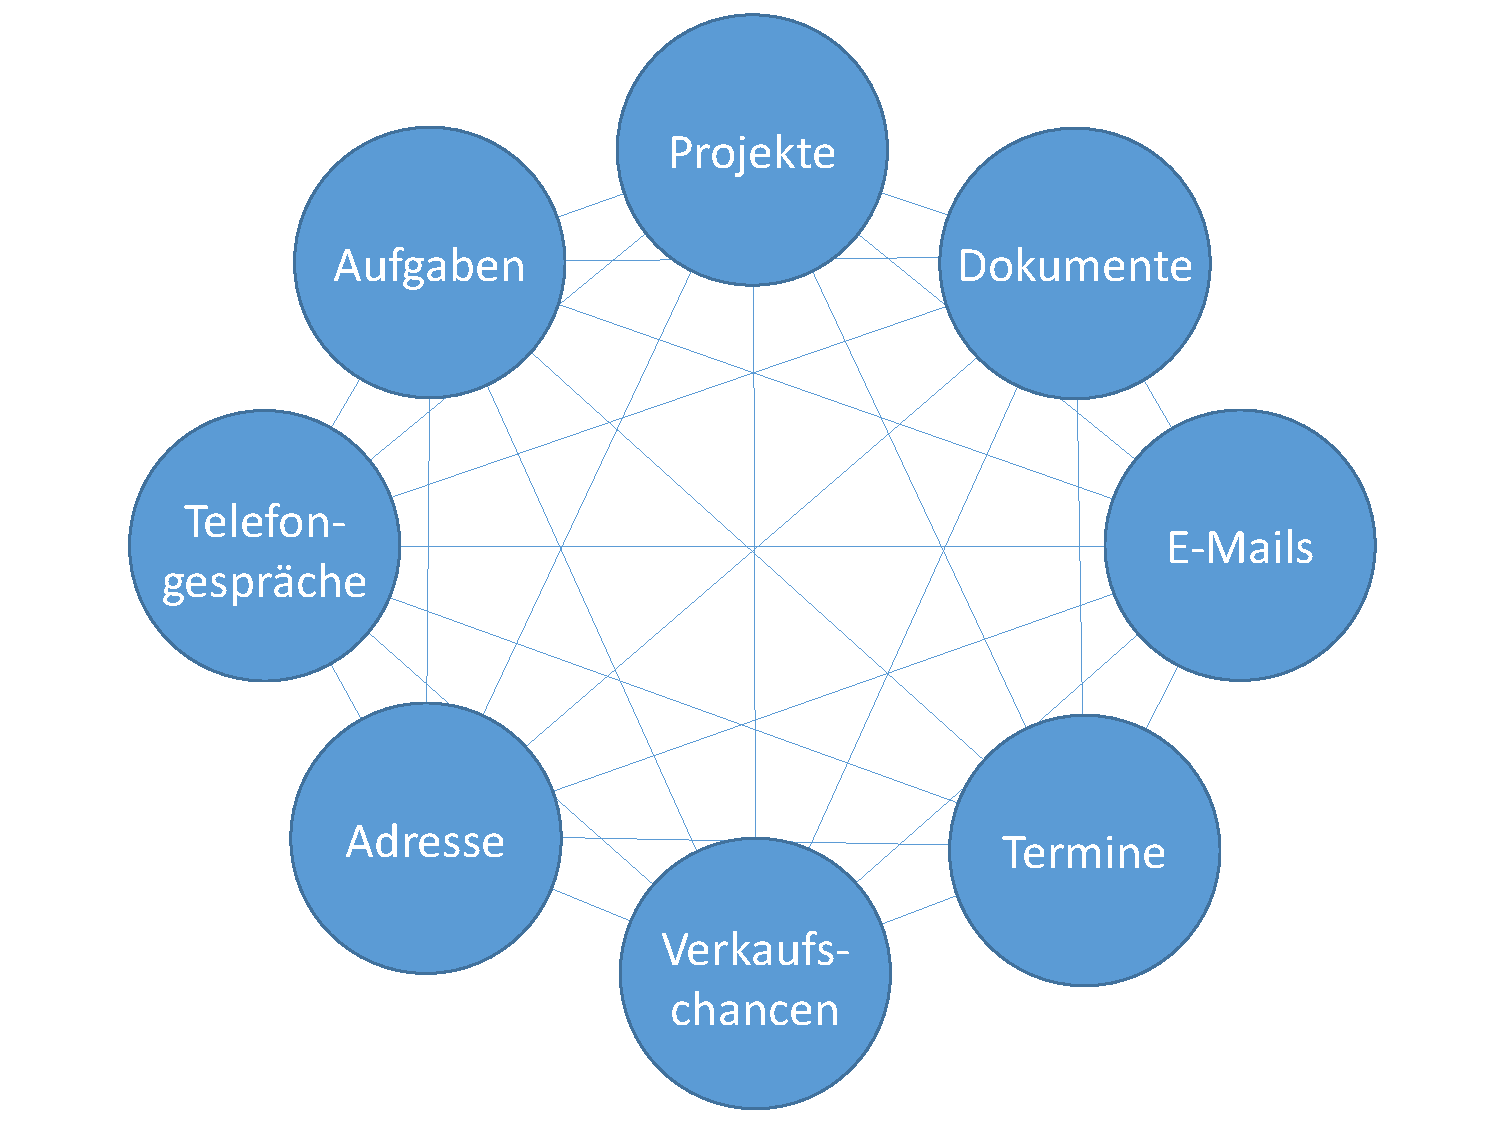
\includegraphics[width=0.5\textwidth, width=0.5\textwidth]{pics/CAS_connections.pdf}
	\caption{Verknüpfungen in CAS genesisWorld}
	\label{picGwCon}
\end{figure}

%% ===========================
\subsection{Architektur}
%% ===========================

Die N-Tier-Architektur von CAS genesisWorld lässt sich in drei wesentliche Bereiche gliedern:

\begin{itemize}

	\item Die Präsentationsclients umfassen alle Dienste, die Informationen in Bildschirmansichten den Benutzern zur Verfügung stellen.
	
	\item Der Applikationsserver umfasst alle Dienste, um die Geschäftslogik zu kapseln, Änderungen zu protokollieren, Benutzerrechte zu prüfen und die aufbereiteten Informationen den Präsentationsdiensten zur Verfügung zu stellen.
	
	\item Die Datenbankschicht umfasst alle Dienste die zur Datenhaltung selbst notwendig sind.
\end{itemize}


%% ===========================
\subsection{Präsentationsschicht \& Logikschicht}
%% ===========================

Der CAS genesisWorld Client existiert in Form einer Windowsanwendung, sowie als mobile Version in Android, Windows Phone, BlackBerry OS und iOS. Die Kommunikation der Clients mit CAS genesisWorld findet über das REST-Protokoll statt \cite{cas2013a}.

Die Funktionalität des CAS genesisWorld Applikationsservers, wurde in Form von COM-Objekten implementiert. Damit stehen dessen Dienste auch Dritten zur Verfügung, die dadurch mit eigenen Applikationen die Informationen von CAS genesisWorld präsentieren oder weiterverarbeiten können. Als Basisdienste stehen der UserService und der DataService zu Verfügung. Für die Anmeldung und Rechteverwaltung ist der UserService zuständig. Der DataService hingegen, als zentraler Dienst für den Zugriff auf die CAS genesisWorld Daten. Die Schnittstelle des DataService wurde an Microsoft ADO angelehnt. Auf den Basisdiensten aufbauend existieren die Geschäftsdienste, in Form der Schnittstellen der BusinessServices. Diese bieten spezielle Funktionen zu den jeweiligen Anwendungsbereichen.

\begin{figure}[H]
	\centering
  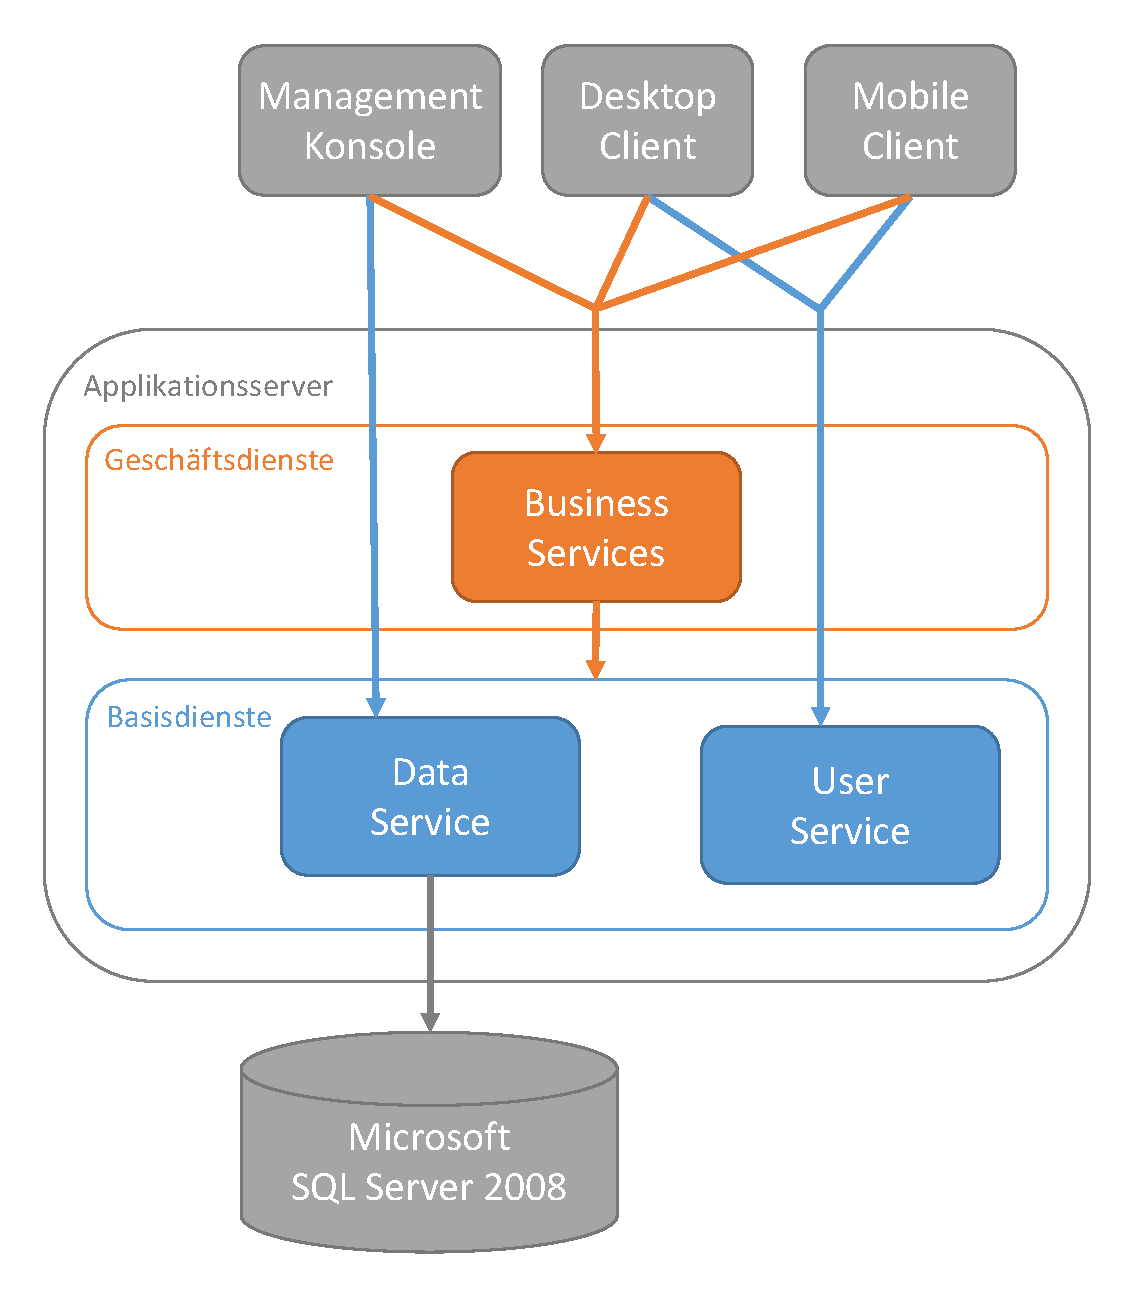
\includegraphics[width=0.6\textwidth, width=0.6\textwidth]{pics/GenesisWorld_Architektur.pdf}
	\caption{Schematische Darstellung der Architektur von CAS genesisWorld}
	\label{gw_Architektur}
\end{figure}

\paragraph{Server-SDK-Plugins}

Die Server-SDK-Plugins bieten die Möglichkeit die Datenverarbeitung, um eine eigene Logik zu erweitern oder zu modifizieren. 

Realisiert werden die PlugIns als COM-Objekte, die ein Plugin-Interface namens \textit{IGWSDKDataPlugIn} implementieren. Das erstellte COM-Objekt wird im Server von CASgenesisWorld registriert. Der Server delegiert bei einer Datenoperation den Aufruf an die für den jeweiligen Datensatztypen registrierten Plugins. In Abbildung \ref{gw_plugin} ist ein Beispiel des Vorgangs dargestellt.

\begin{figure}[H]
	\centering
  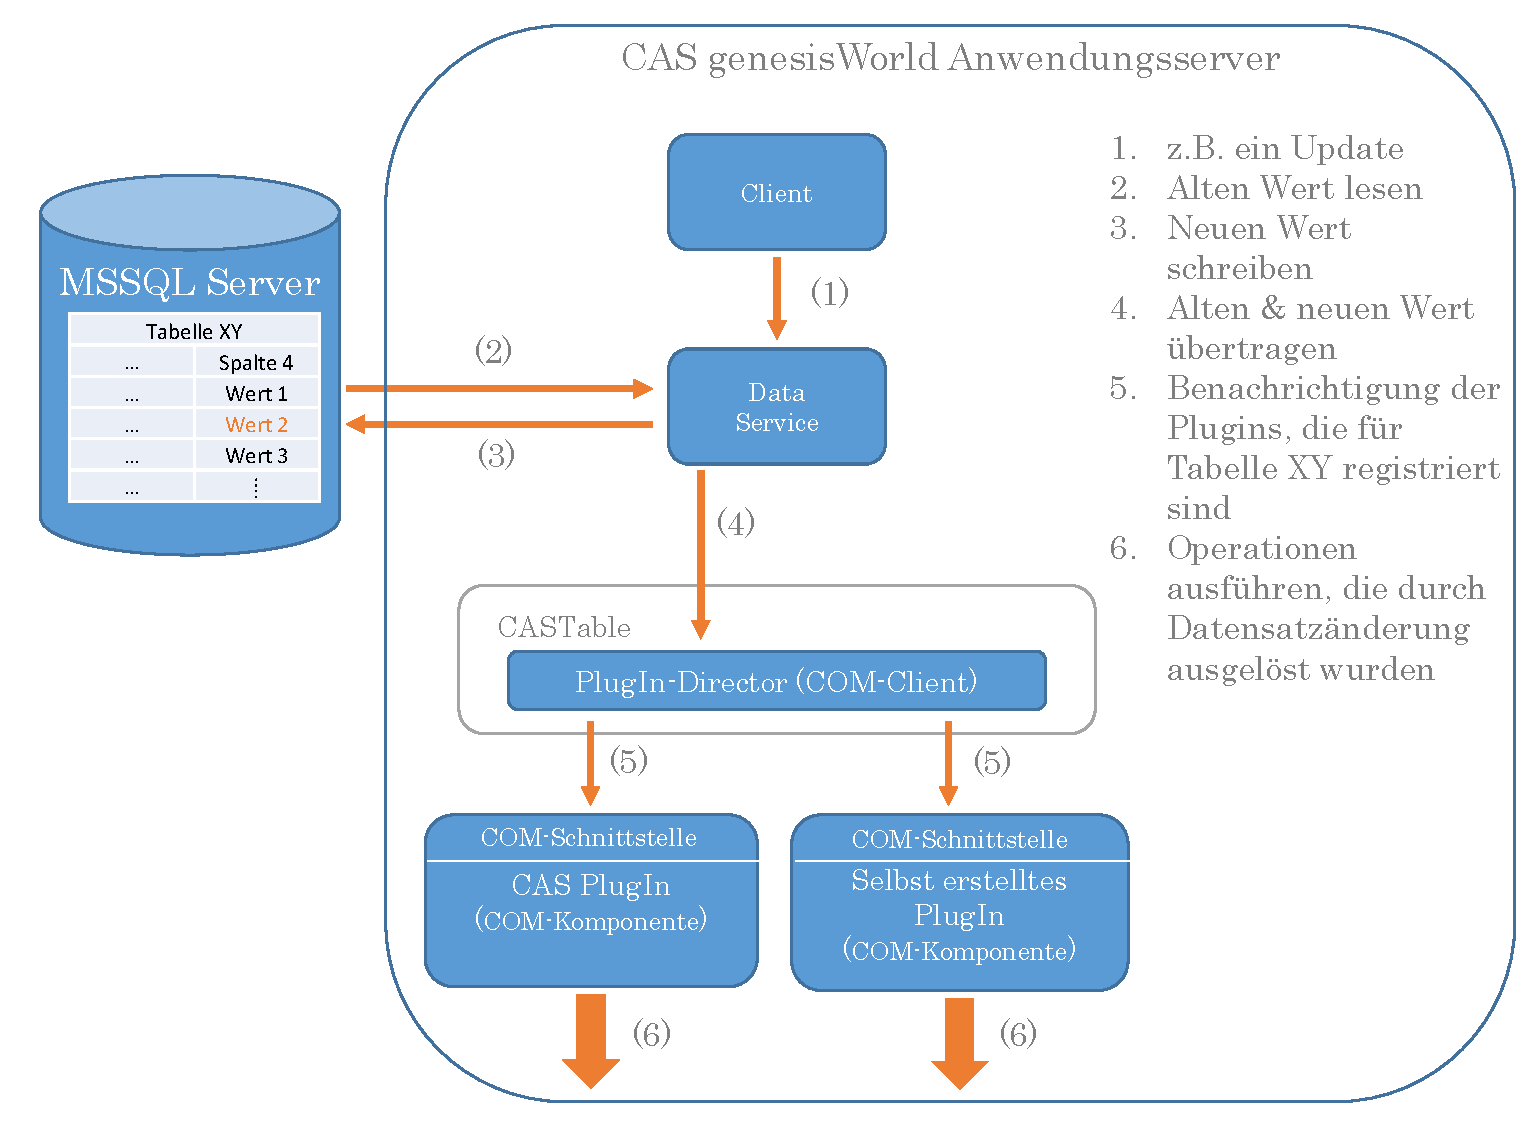
\includegraphics[width=1.0\textwidth, width=1.0\textwidth]{pics/analyse_plugins.pdf}
	\caption{Beispiel zur Benachrichtigung von Plugins anhand eines Ablaufs bei einem Update}
	\label{gw_plugin}
\end{figure}

Im Allgemeinen stehen in den COM-Schnittstellen der Plugins, jeweils alle Felder eines Datensatz-Typen zur Verfügung, sowie die individuelle Teilmenge der Felder mit neuen Werten. In den Plugins besteht somit die Möglichkeit, alte bzw. neue Werte von Feldern zu untersuchen und zu vergleichen und auf das Ergebnis zu reagieren.

Die Werteteilmenge des aktuell verarbeiteten Datensatzes kann verändert, d.h. erweitert oder reduziert werden und die Werte selber sind änderbar. Darüber hinausgehend sind auch automatisierte Aktionen realisierbar, die weitere Datensätze betreffen. So könnten z.B. abhängig von den Eingangswerten einer neu angelegten Adresse, neue Aufgaben angelegt und mit Inhalt versehen werden. Einige automatische Datenoperationen von CAS genesisWorld werden über CAS-Plugins realisiert, die mit den SDK-Plugins verwandt sind.

%% ===========================
\subsection{Datenhaltungsschicht}
\label{ch:Systemanalyse:sec:genesisWorld:subsec:db}
%% ===========================

Die Datenhaltungsschicht enthält einen Microsoft SQL Server 2008 (MSSQL). Der SQL Server ist ein relationales Datenbankmanagementsystem (RDBMS) von Microsoft, dass für den Einsatz im Konzernumfeld konzipiert wurde. MSSQL verwendet T-SQL (Transact-SQL), eine Erweiterungen von Sybase und Microsoft, der mehrere Funktionen zum SQL-Standard hinzufügt \cite{tech2013}. Weiterhin unterstützt MSSQL standardisierte Datenbankschnittstellen, wie Open Database Connectivity (ODBC) und Java Database Connectivity (JDBC).
  
In den meisten relationalen Datenbanken werden Beziehungen über Primär- und Fremdschlüssel abgebildet. In der CAS genesisWorld Datenbank werden nur Primärschlüssel eingesetzt. Die Beziehungen werden nicht wie sonst in mehreren Zwischentabellen realisiert, sondern in einer einzigen Tabelle, die \textit{TableRealtion}. Abbildung \ref{gw_2} zeigt eine beispielhafte, schematische Darstellung der \textit{TableRealtion}.

\begin{figure}[ht]
	\centering
  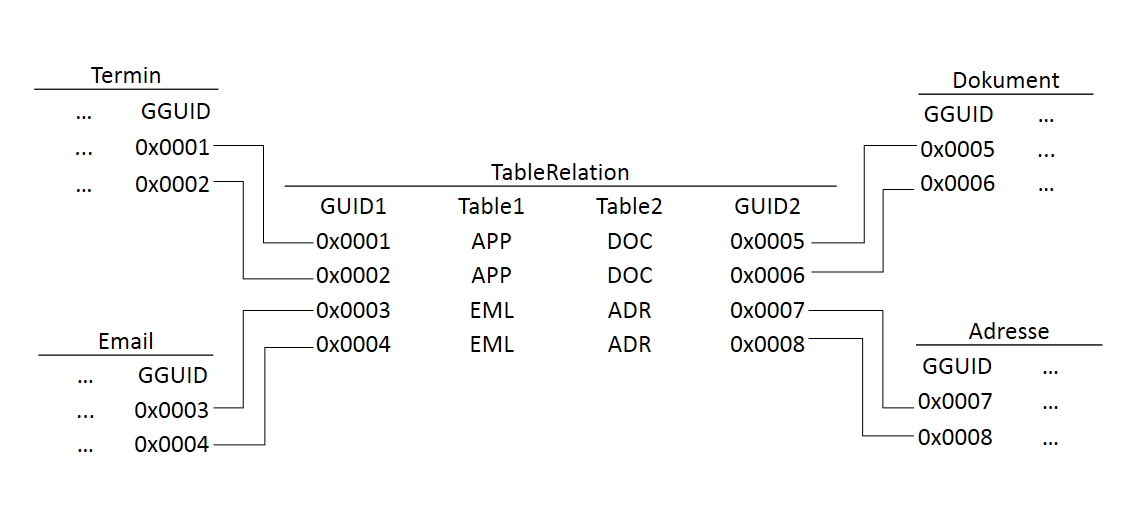
\includegraphics[width=0.9\textwidth, width=0.9\textwidth]{pics/gW_tablerealtion.png}
	\caption{Funktionsweise von RelationTable anhand eines Beispiels}
	\label{gw_2}
\end{figure}

Die Spalten \textit{GUID1} und \textit{GUID2} beinhalten die jeweiligen Primärschlüssel der in Beziehung zu setzenden Tabellen. Als Zuordnungsmerkmal für die \textit{GGUID}s zu ihren Tabellen dienen die Spalten \textit{TableSign1} und \textit{TableSign2}, deren Inhalt aus Kürzeln der Tabellennamen besteht. Möglich wird die Verknüpfung verschiedener Tabellen durch einen besonderen Primärschlüssel. Dieser wird für jede neue Zeile generiert und ist in der gesamten Datenbank eindeutig. Er wird als Genesis Global Unique Identifier (GGUID) bezeichnet und ist eine global eindeutige Zahl bestehend aus 128 Bit. Jede Tabellen besitzen eine Spalte mit \textit{GGUID}s, welche eine Datenintegrität in der gesamten Datenbank sicherstellt.

%% ===========================
\section{Anforderungsanalyse}
\label{ch:Systemanalyse:sec:Anforderungsanalyse}
%% ===========================

Während der Anforderungsanalyse wird ermittelt welche Eigenschaften und Fähigkeiten das System zur Erreichung der Ziele benötigt. Wir unterscheiden bei der Einteilung der Anforderungen zwischen Funktionalen und Nichtfunktionalen. Beim erst genannten wird die Funktionalität des zu erstellenden Systems beschrieben, wohingegen alle anderen Anforderungen unter letzteres Fallen. 

Bevor wir auf die funktionalen und nichtfunktionalen Anforderungen eingehen, wird das umzusetzende Szenario näher beschrieben. Mit dem zu entwickelndem System soll eine Bewertung der Beziehung zwischen Personen aus CAS genesisWorld ermöglicht werden. Indessen soll ermittelt werden, welche Personen die ausgeprägteste Beziehung zu einer vorher bestimmten Person besitzen. Die Bewertung der Ausprägung basiert dabei auf der Häufigkeit des Kontakts mit der Person. Die Häufigkeit des Kontakts wird dabei anhand von fünf verschiedenen Merkmalen ermittelt. Zu einem wird der E-Mail-Verkehr unter den Personen für die Betrachtung herangezogen. Überdies werden die Telefonate unter den Personen miteinbezogen. Außerdem spielen nachvollziehbare Treffen (Termine) zwischen den Personen eine Rolle. Unter Personen geteilte Dokumente werden auch als Merkmal festgesetzt. Das letzte Merkmal stell die Verkaufschance gegenüber einem Kunden dar. Wie ausgeprägt letztendlich die Beziehung zu einer anderen Person ist, wird anhand der Anzahl solcher Merkmale ermittelt. Auf die fünf Merkmale wird im weiteren Verlauf der Arbeit nur noch mit dem Begriff "Verbindungsmerkmale" verwiesen. Weiterhin ist die Betrachtung nicht auf die gesamte Dauer des Kontakts vorgesehen, sondern auf festgelegte Zeitspannen. Beispielsweise sollte es möglich sein, die Ergebnisse auf den Zeitraum vom 01.02 bis 10.08.2013 einzugrenzen. Zusätzlich sollten weitere Eingrenzungen möglich sein, die im Folgenden Abschnitt beschrieben werden.

%% ===========================
\subsection{Funktionale Anforderungen}
%% ===========================

Folgende funktionale Anforderungen wurden erhoben:

\begin{itemize}
\item Ermittlung der Anzahl von Verbindungsmerkmalen ausgehend von einer Personen, zu allen anderen Personen im CRM-System

\item Ranking der Personen basierend auf der Summe von Verbindungsmerkmalen, die von der Ausgangsperson ausgehen

\item Abfrageergebnis soll die Summe der gesamten Verbindungsmerkmale zu den jeweiligen Person enthalten, sowie die Summe der einzelnen Verbindungsmerkmale

\item Begrenzung des Ergebnisses hinsichtlich der Anzahl an Personen

\item Möglichkeit zum eingrenzen des Ergebnisses auf einen festen Zeitraum

\item Ein- und Ausblenden von Suchkriterien, ohne eine neue Anfrage senden zu müssen

\item Gewichtung der Suchkriterien durch den Nutzer

\item Gewichtung von Zeitspannen durch den Nutzer

\item Filterung der Ergebnismenge durch:	
	\begin{itemize}
	\item Ausschließen von Personen oder Eingrenzen auf Personen
	\item Städte und/oder Länder der Personen
	\item Verringern auf Personen, die einem Unternehmen zugeordnet sind 
	\item Beschränken auf Kontaktpersonen von Unternehmen
	\item Begrenzen auf Kontaktpersonen die keinem Unternehmen angehören
	\item Vermindern um Personengruppen
	\end{itemize}
\end{itemize}

%% ===========================
\subsection{Nichtfunktionale Anforderungen}
%% ===========================

Folgende nicht nichtfunktionale Anforderungen wurden erhoben:

\begin{itemize}
	
	\item Eine Rechnerinstanz für Datenbankserver und Applikationsserver 
	
	\item Sehr hohe Verarbeitungsgeschwindigkeit (unter einer Sekunde)
	
	\item Lose Kopplung (zwischen Logik und Darstellung)
	
	\item Portabilität
	
	\item Graphische Darstellung des Ergebnisses
	
	\item keine zusätzliche Kosten

\end{itemize}

%% ===========================
\section{Ermittlung relevanter Daten}
\label{ch:Systemanalyse:sec:Information}
%% ===========================

Die Datenbank der CAS Software AG umfasst 398 Tabellen, die zusammen wiederum 11.620 Spalten beinhalten. Aufgrund einer fehlenden Dokumentation über die Umsetzung der Anwendungsschicht und der Abwesenheit von fehlenden, definierten Beziehungen innerhalb der Datenbank wurde ein eigenes Verfahren zur Ermittlung der Beziehungen entwickelt. 

Für den Ausgangspunkt der Suche wurde eine Tabelle namens \textit{SysUser} verwendet. Sie beinhaltet jeden Benutzer des Systems. Ihre Eignung beruht auf der Annahme, dass bei der Bewertung von Beziehungen zwischen Personen, die Person selbst dabei immer den Ausgangspunkt der Suche darstellt. Aus Datenbanksicht bedeutet dies, dass zuerst eine Tupel der \textit{SysUser} Tabelle mit ihrer \textit{GGUID} herangezogen wird. Die \textit{GGUID} ist dabei der erste Wert nachdem in der gesamten Datenbank gesucht wird. Sobald alle Tabellen gefunden wurden, die den Wert beinhalten, werden deren \textit{GGUID}s für die weitere Suche verwendet. Die Menge der Suche wird nach jedem Schritt, um die Teilmenge der bereits gefundenen Tabellen verringert. Die Suche wird abgebrochen, sobald die Suchmenge keine Werte mehr aufweist oder keine Tabellen mehr mit den entsprechenden Werten gefunden wurden. Durch dieses Vorgehen erhält man am Ende alle Beziehungen, aufbauend auf der Annahme, dass die \textit{GGUID} als Wert für die Referenzierung genutzt wurde. In Abbildung \ref{gw_schema_alt} ist ein schon auf das Wesentliche reduzierter Ausschnitt des Ergebnisses zu sehen. 

Von den ursprünglichen 398 Tabellen sind nur noch 17 übrig geblieben, auf die im weiteren Verlauf eingegangen wird. Alle Tabellen enthalten in der ursprünglichen Form wesentlich mehr Spalten und wurden der Übersicht halber entfernt. Tabelle \textit{SysUser} besitzt drei Spalten die von Bedeutung sind. Eine davon ist die \textit{GGUID}, die im Folgenden nicht weiter erwähnt wird, da sie jede Tabelle enthält. Die \textit{OID} wird für jeden Nutzer einmalig vergeben und wird in anderen Tabellen als Zuordnungsmerkmal verwendet. \textit{LoginName} ist wie der Name schon sagt, der Benutzername des Nutzers und kann beim anmelden auf der Oberfläche verwendet werden. 

Aufgrund der Anforderung von Filterung der Ergebnisse durch Gruppen, wurden die Tabellen \textit{SysGroupMember} und \textit{SysGroup} hinzugezogen. \textit{SysGroup} besitzt eine \textit{GID}, die sich bei Gruppen genauso verhält, wie die \textit{OID} bei Personen. Das Attribut \textit{GroupName}, wird für die Anzeige an der Oberfläche benötigt. Mithilfe dessen der Nutzer nachvollziehen kann, welche Gruppe er gerade ausgewählt hat. \textit{SysGroupMember} stellt die Auflösungstabelle zwischen \textit{SysUser} und \textit{SysGroup} dar. Die Spalte \textit{GroupID} beinhaltet Werte aus der \textit{GGUID} Spalte der \textit{SysGroup} Tabelle. \textit{MemberID} folgt dem selben Ansatz, allerdings werden die \textit{GGUID}s der \textit{SysUser} Tabelle verwendet. Hinsichtlich der Logikschicht wird die Spalte \textit{InsertTimestamp} für Veränderungen innerhalb der Gruppen benötigt.

Die \textit{Address0} Tabelle wird für die Filter Anforderungen benötigt. \textit{Town1} und \textit{Country1} geben die Stadt sowie das Land an, in der die Person ansässig ist. Zur Ermittlung, ob eine Person eine Kontaktperson, Mitarbeiter oder eine Firma repräsentiert, werden die Attribute \textit{gwIsContact}, \textit{gwIsEmployee} und \textit{gwIsCompany} benötigt. \textit{ChristianName} und \textit{Name} beinhalten den Vor- und Nachname der Person, welche für die Zuordnung der Ergebnisse an der Benutzeroberfläche hilfreich sind. Im Voraus ist zu sagen, dass nicht alle Telefongespräche über die dafür bestimmten Tabellen ermittelt werden können. Deswegen werden die Attribute \textit{PhoneFieldStr1-10} benötigt, mithilfe derer eine Zuordnung möglich ist. 

Die \textit{TableRelation} enthält, wie in Abschnitt \ref{ch:Systemanalyse:sec:genesisWorld:subsec:db} behandelt, die Beziehungen der Datenbank. Beispielsweise kann für die \textit{GUID1} die \textit{GGUID} der \textit{SysUser} verwendet werden. Mithilfe der \textit{GUID2} können die mit der Person verknüpften Termine, Verkaufschancen, Telefonate, Dokumente und E-Mails anschließend bestimmt werden. \textit{TableSign1} und \textit{TableSign2} können zur Identifikation der jeweiligen Tabellen verwendet werden.

\begin{figure}[H]
	\centering
  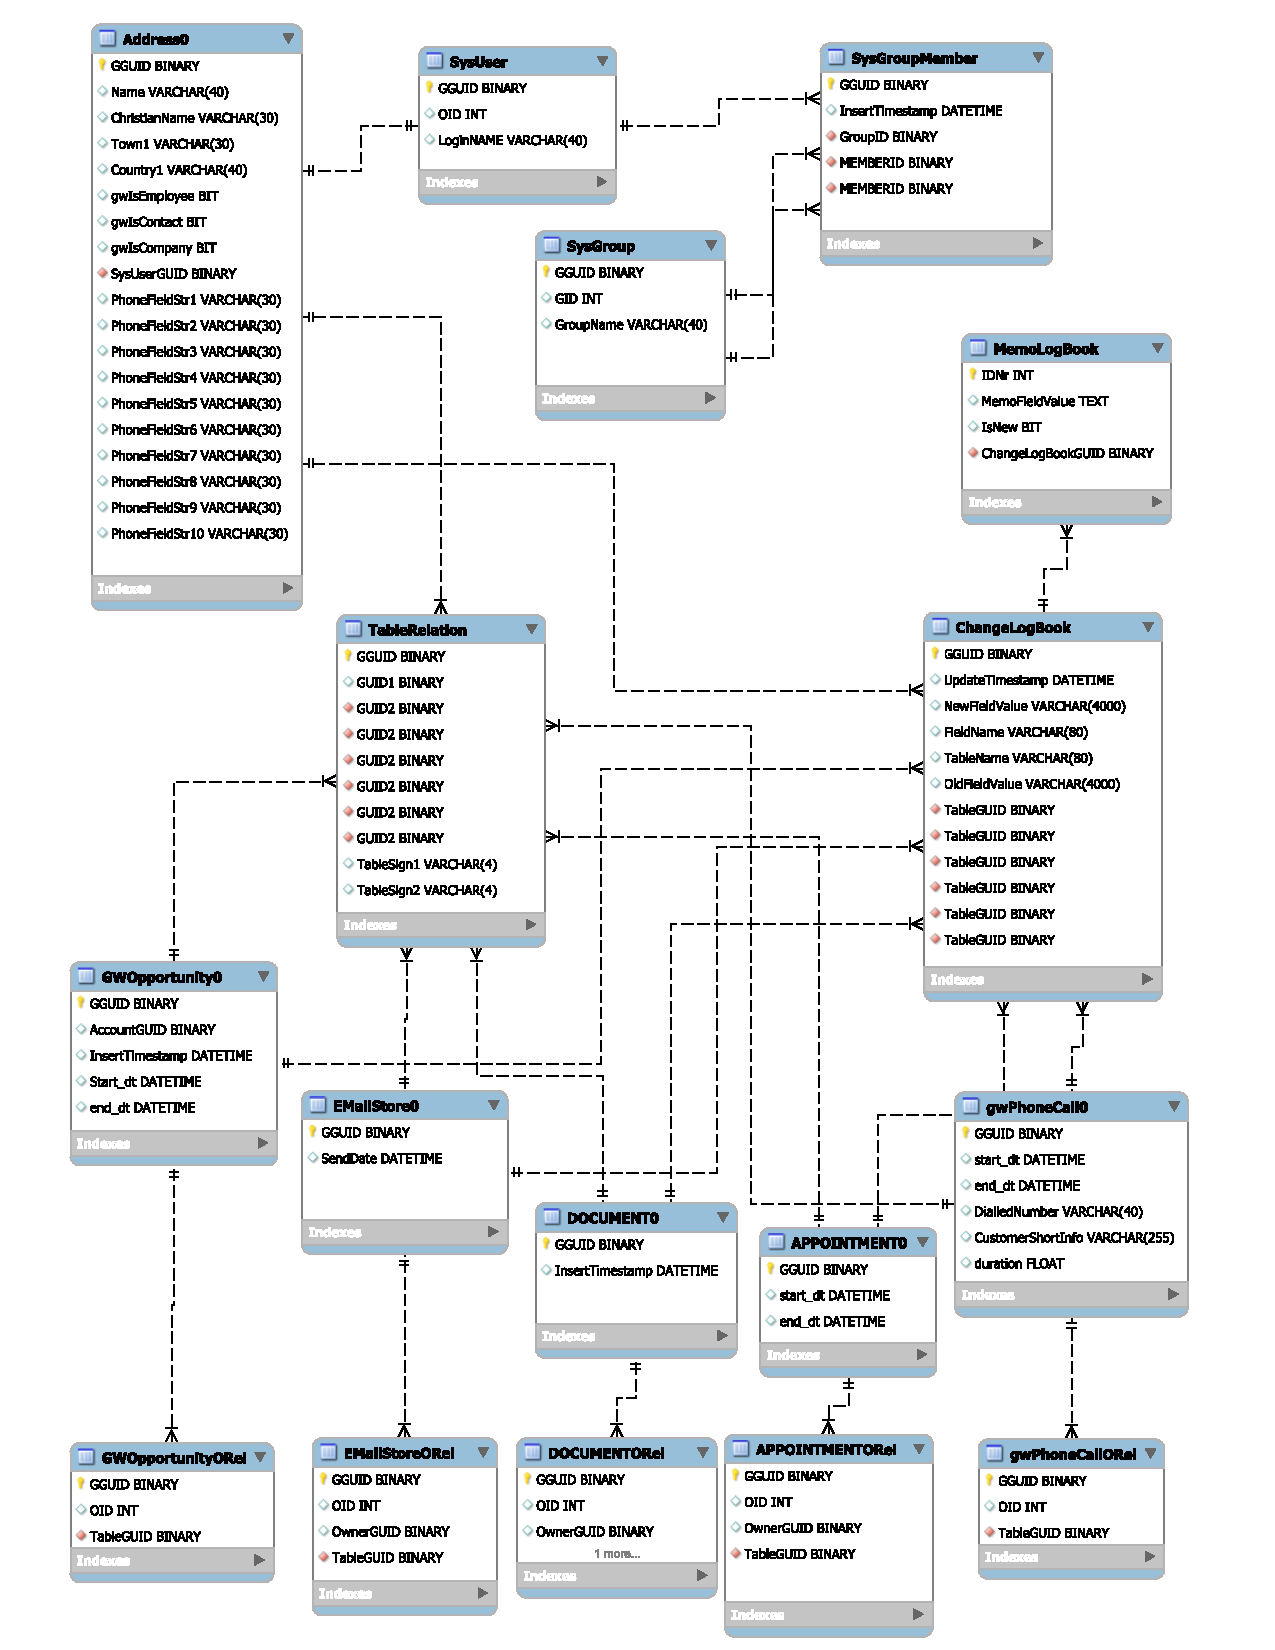
\includegraphics[width=1.0\textwidth]{pics/schema_alt.pdf}
	\caption{Auszug aus dem Schema des MSSQL 2008}
	\label{gw_schema_alt}
\end{figure}

\textit{GWOpportunity0} enthält alle Informationen über die jeweiligen Verkaufschancen. Das Attribut \textit{InsertTimestamp} wird zur Feststellung des Erzeugungszeitpunktes benötigt. \textit{Start\_dt} und \textit{end\_dt} legen den Zeitraum der Verkaufschance fest. Der Besitzer einer Verkaufschance wird über die \textit{AccountGUID} bestimmt. Mit \textit{EMailStore0}, \textit{Document0} \textit{Appointment0} und \textit{gwPhoneCall0} verhält es sich wie mit \textit{GWOpportunity0}. Bei \textit{EMailStore0} ist zu erwähnen, dass \textit{SendDate} zur zeitlichen Einordnung verwendet werden kann. Das Attribut \textit{DialledNumber} der Tabelle \textit{gwPhoneCall0} wird zum Vergleich  mit der in der Adresse hinterlegten Telefonnummer benötigt. Zur Überprüfung ob das Telefonat über einen Tag hinausging, wird das Attribut \textit{duration} herangezogen.

Bis jetzt galt die Annahme, dass alle Beziehungen über die\textit{TableRelation} bestimmt werden können. Dies trifft allerdings nicht für alle Beziehungen zu. Dort werden nur, die an der Oberfläche manuell verknüpften Objekte aufbewahrt. Die restlichen Beziehungen können aus den ORel-Tabellen ermittelt werden. Jeder dieser Tabellen enthält eine \textit{OID} bzw. \textit{GID}, die zur Bestimmung der beteiligten Personen und/oder Gruppen dienen.

Eine Betrachtung basierend auf Zeitspannen, impliziert Veränderungen der Daten über die Zeit gesehen. Um diese Änderungen zu erfassen wird die Tabelle \textit{ChangeLogBook} benötigt. \textit{NewFieldValue} enthält den neuen Wert eines Feldes. Wohingegen \textit{OldFieldValue} den alten Wert des Feldes repräsentiert. Die Spalte des geänderten Wertes ist in \textit{FieldName} hinterlegt. Der Name der Tabelle ist der Spalte \textit{TableName} zu entnehmen. Die Referenzierung auf eine Tupel wird in der Spalte \textit{TableGUID} vorgenommen. Aus Gründen des Speicherplatzverbrauchs werden nur varchar Datentypen bei Zeichenfolgen verwendet. Varchar ist allerdings auf 4000 Zeichen limitiert. Falls Zeichenfolgen diese Grenze überschreiten, werden diese in der Tabelle \textit{MemoLogBook} abgelegt. Dort wird der Datentyp Text verwendet, der eine maximale Zeichenfolgenlänge von $2^{31}-1$ (2.147.483.647) erlaubt.
%% ===========================
\chapter{Analyse ausgewählter Datenbanken}
\label{ch:AnalyseDatenbanken}
%% ===========================

Ein Ziel der Arbeit ist hohe Geschwindigkeiten in der Beantwortung der Benutzeranfragen zu erreichen. Die maßgebende Komponente in diesem Fall ist die Datenbank. Sie führt die zeitintensiven Ermittlungen, Berechnungen und Filterungen des Gesamtsystems durch. Um Anhaltspunkte für mögliche Kandidaten zu bekommen, sollen im folgenden eine Reihe bekannter Datenbanken vorgestellt und gegenübergestellt werden. Bei der Zusammenstellung wurde darauf geachtet, dass ein möglichst weites Spektrum unterschiedlicher Datenbanken ausgewählt wurde.

%% ===========================
\section{Datenbanken}
\label{ch:AnalyseDatenbanken:sec:Datenbanken}
%% ===========================

Im folgenden werden nun einige Datenbanken vorgestellt. Dabei wird insbesondere versucht einen guten Überblick über die Charakteristika der einzelnen Datenbanken zu geben. Der dahinter stehende Gedanken ist, dass der Vergleich und die Auswahl, besser nachvollziehbar werden. 

%% ===========================
\subsection{CouchDB}
\label{ch:AnalyseDatenbanken:sec:Datenbanken:subsec:CouchDB}
%% ===========================

CouchDB \cite{couch2013} ist eine dokumentorientierte Datenbank, die seit Anfang 2008 unter der  Apache-Lizenz verbreitet wird. In CouchDB werden die Daten in Collections anstatt in Tabellen abgelegt. Collections bestehen aus einer Sammlung von unabhängigen Dokumenten. Jedes Dokument verwaltet seine eigenen Daten in einem freien Schema. 
Ein Dokument hat Feldwerte, die Datentypen (Text, numerisch oder boolean) oder Datenstrukturen (ein Dokument oder Liste) beinhalten. Abfragen werden mit views zum Filtern der Dokumente ausgeführt. In CouchDB werden für Indizes B-Bäume verwendet, sodass die Ergebnisse sortiert und Wertebereich-Anfragen ausgeführt werden können. Abfragen können parallel über mehrere Knoten mit einem MapReduce Mechanismus verteilt werden. CouchDB erreicht Skalierbarkeit durch asynchrone Replikation, nicht durch Fragmentierung. Lesezugriffe können auf beliebigen Server stattfinden, wenn Aktualität keine Rolle spielt. Updates hingegen müssen an alle Server weitergegeben werden.
CouchDB unterscheidet sich von anderen Systemen durch die Akzeptanz von eventueller Konsistenz. CouchDB implementiert MVCC auf einzelne Dokumente, mithilfe einer Sequenz-ID, die für jede Version eines Dokuments generiert wird. CouchDB benachrichtigt eine Anwendung, wenn jemand anderes das Dokument aktualisiert hat, seitdem es zuletzt auf der Datenbank abgelegt wurde. Die Anwendung kann dann versuchen, die Updates zu kombinieren oder das Update zu wiederholen, um die Daten zu überschreiben. CouchDB erfüllt damit im lokalen Einsatz die ACID-Eigenschaften. Jede Transaktion ist eine in sich abgeschlossene Operation, die entweder ganz oder gar nicht ausgeführt wird. Es treten keine Seiteneffekte zwischen den Anfragen auf. Außerdem wird die Datenbank immer in einem konsistenten Zustand hinterlassen.

%% ===========================
\subsection{MongoDB}
\label{ch:AnalyseDatenbanken:sec:Datenbanken:subsec:MongoDB}
%% ===========================

MongoDB ist ein in C++ geschriebener, Open Source Document Store \cite{books/daglib/0025185}. Es besitzt einige Ähnlichkeiten mit CouchDB. Beide bieten Indizes auf Collections, sind lockless, und bieten einen Abfragemechanismus für Dokumente. Es gibt jedoch wichtige Unterschiede:

\begin{itemize}

	\item MongoDB unterstützt automatische Fragmentierung, die Dokumente über Server verteilt.
	\item Dynamische Abfragen mit automatischer Verwendung von Indizes werden von MongoDB unterstützt. In CouchDB werden, durch das Schreiben von map-reduce-views, Daten indiziert und gesucht.
	\item CouchDB nutzt MVCC bei Dokumenten, wohingegen MongoDB atomare Operation auf Feldern nutzt   

\end{itemize}

MongoDB speichert Daten in einem JSON-ähnlichen, binären Format namens BSON. BSON unterstützt boolean, integer, float, Datum, String-und Binär-Typen. Die Treiber der Clients verschlüsseln die lokalen Dokumentdatenstrukturen in das BSON Format und senden es an den MongoDB Server. Weiterhin unterstützt MongoDB die GridFS-Spezifikation für große binär Dateien, wie z.B. Filme oder Bilder. MongoDB unterstützt Master-Slave-Replikation mit automatischem Failover und Recovery. Replikation (und Wiederherstellung) basieren auf dem Prinzip der Fragmentierung. Collections werden über einen benutzerdefinierten Schlüssel automatisch fragmentiert. Die Replikation ist asynchron umgesetzt um höhere Leistung zu erzielen, jedoch können Updates dadurch bei einem Crash verloren gehen. 

%% ===========================
\subsection{Voldemort}
\label{ch:AnalyseDatenbanken:sec:Datenbanken:subsec:Voldemort}
%% ===========================

Projekt Voldemort \cite{vod2013} ist eine verteiltec Key-Value-Store Datenbank (entwickelt von LinkedIn), welche ein hoch skalierbares Speicher-System zur Verfügung stellt. Voldemort repliziert sich durch automatisches partitionieren und anschließendes verteilen der Daten auf multiple Server. Jeder Server stellt einen unabhängigen Knoten im System dar, der für die Verwaltung seiner Daten verantwortlich ist. Dadurch existiert kein Single Point of Failure im Cluster. Ein solches Daten Model erlaubt eine Cluster Expansion, ohne eine Neuverteilung der Daten vornehmen zu müssen. In Voldemort können verschiedene Storage Systeme, wie BerkeleyDB oder MySQL eingesetzt werden. 

Für die Ablage der Daten werden in Voldemort sogenannte Stores verwendet. Unterstützt werden lediglich Key-Value Ablagen. Jedoch können die Werte auch komplexe Datenstrukturen wie Maps oder Listen beinhalten. Voldemort stellt für die Datenmanipulation vier verschiedene Operatoren zur Verfügung:

\begin{itemize}

	\item PUT (Key,Value)
	\item GET (Key)
	\item MULTI-GET (Keys)
	\item DELETE (Key, Version) 

\end{itemize}

Eine Möglichkeit für Bereichsabfragen ist nicht vorhanden. Der Parameter Version, im DELETE-Operator, dient der Unterscheidung der Datensätze und ist auf das Verfahren zur Gewährleistung der Konsistenz zurückzuführen. Zur Gewährleistung der eventuellen Konsistenz werden Timestamps und die Vector Clock Technik eingesetzt. Neben der eventuellen Konsistenz bietet Voldemort einen Betrieb mit starker Konsistenz an.       

%% ===========================
\subsection{Redis}
\label{ch:AnalyseDatenbanken:sec:Datenbanken:subsec:Redis}
%% ===========================

Redis \cite{red2013} ist ein In-Memory-, Key-Value-Store mit einer Option für Persistenz. Redis Datenmodell unterstützt Strings, Hashes, Listen, Mengen und sortierte Mengen. Obwohl Redis für In-Memory-Daten entworfen wurde, kann je nach Anwendungsfall ein (semi-)persistenter Bestand angelegt werden. Entweder durch Momentaufnahmen der Daten und anschließendes ablegen auf der Festplatte, in regelmäßigen Abständen oder durch aufzeichnen eines Logs mit allen ausgeführten Operationen. Weiterhin kann Redis mit einer Master-Slave-Architektur repliziert werden. Genau wie andere Key-Value-Stores implementiert Redis insert, delete und lookup Operatoren. Weiterhin setzt Redis atomare Updates durch locking um. 

%% ===========================
\subsection{HBase} 
\label{ch:AnalyseDatenbanken:sec:Datenbanken:subsec:HBase}
%% ===========================

HBase ist eine verteiltes, Open Source Column Store Datenbanksystem, welches auf Googles BigTable basiert \cite{Chang:2006:BDS:1267308.1267323}. HBase läuft auf Apache Hadoop und Apache ZooKeeper  \cite{Hunt:2010:ZWC:1855840.1855851} und verwendet das Hadoop Distributed Filesystem (HDFS) \cite{Shvachko:2010:HDF:1913798.1914427}, um Störung-Toleranz und Replikation zu bieten. Zeilen Operationen sind in HBase atomar, mit Sperren auf Zeilenebene und Transaktionen. Partitionierung und Verteilung sind transparent, da es kein clientseitiges Hashing oder feste Schlüsselräume wie in einigen NoSQL-Systemen gibt. 
Insbesondere stellt es lineare und modulare Skalierbarkeit, sowie streng konsistenten Datenzugriff und automatische, konfigurierbare Fragmentierung von Daten zu Verfügung. Auf Tabellen kann in HBase über eine API zugegriffen werden. Sie können jedoch auch als Ein-und Ausgangsdaten für MapReduce-Jobs in Hadoop verwendet werden. Anwendungen speichern in HBase Daten in Tabellen, die aus Zeilen und Spalten-Familien bestehen. Spalten-Familien beinhalten wiederum Spalten. Darüber hinaus kann jede Zeile einen anderen Satz von Spalten beinhalten. Alle Spalten sind mit einem vom Benutzer bereitgestellten Schlüsselspalte indiziert und in Spalten-Familien gruppiert.

%% ===========================
\subsection{Cassandra} 
\label{ch:AnalyseDatenbanken:sec:Datenbanken:subsec:Cassandra}
%% ===========================
Apache Cassandra ist eine verteilte Column-Store Datenbank die von Facebook entwickelt wurde \cite{Lakshman:2010:CDS:1773912.1773922}. Sie ist eine Mischung aus Amazon Dynamo und Google BigTable, wodurch sie des öfteren als Hybrid zwischen Key-Value-Store und Column Store bezeichnet wird. Cassandra wurde entwickelt, um große Daten-Workloads über mehrere Knoten, ohne Single Point of Failure zu behandeln. Die Architektur ist von der Annahme geprägt, dass System-und Hardware-Fehler auftreten können und auch wirklich auftreten. Cassandra behandelt das Problem von Fehlern durch Verwendung eines Peer-to-Peer-System, in dem alle Knoten gleich sind und die Daten von allen Knoten des Clusters verteilt werden. Jeder Knoten tauscht Informationen über das Cluster im Sekundentakt aus. Ein Commit-Log auf jedem Knoten fängt Schreibaktivität ab, um Datenhaltbarkeit zu gewährleisten. Daten werden auch auf eine In-Memory Struktur geschrieben, die memtable. Sobald die Speicherstruktur voll ist, werden die Daten in eine Datei auf die Festplatte geschrieben, auch SSTable genannt. Alle Schreibvorgänge werden automatisch aufgeteilt und auf mehrere Cluster repliziert. 

Cassandras Datenmodell basiert auf einem partitionierten Row-Store mit eventueller Konsistenz. Zeilen werden in Tabellen organisiert, wobei die erste Komponente des Primärschlüssels einer Tabelle der Partition-Schlüssel ist. Innerhalb einer Partition werden Zeilen nach den verbliebenen Spalten des Primärschlüssels geclustert. Andere Spalten können getrennt vom Primärschlüssel indiziert werden. Was Cassandra von HBase unterscheidet sind ihre Spalten, die in einer verschachtelten Weise in Spalten-Familien gruppiert werden können.

Ein weiteres Unterscheidungsmerkmal stellt die Möglichkeit zur Angabe der Konsistenz Anforderung dar, die zum Zeitpunkt der Abfrage angebbar ist. Weiterhin ist Cassandra ein schreiborientiertes System, während HBase entwickelt wurde, um hohe Leistung für intensive Leseaufgaben zu erzielen.

%% ===========================
\subsection{VoltDB} 
\label{ch:AnalyseDatenbanken:sec:Datenbanken:subsec:VoltDB}
%% ===========================

VoltDB \cite{volt2013a} ist ein ACID-konformes, relationales In-Memory-Datenbanksystem, abgeleitet vom Forschungsprototyp H-Store \cite{kallman08}. Da VoltDB auf dem Ansatz der relationalen Algebra beruht zählt es zu den NewSQL-Datenbanken. Es basiert auf einer Shared-Nothing-Architektur und wurde entwickelt, um auf einem Cluster mit mehreren Knoten zu laufen. Erreicht wird dies indem die Datenbank in getrennte Partitionen aufgeteilt wird, bei dem jeder Knoten Besitzer und Verantwortlicher für die jeweiligen Partitionen ist. Durch Verwendung von gespeicherten Prozeduren als Transaktionseinheit werden Round-Trip-Messages zwischen SQL Anfragen verhindert. Die Anfragen werden seriell in einem einzigen Thread ausgeführt, sodass kein locking and latching mehr notwendig ist \cite{volt2013b}. Die Daten werden im Arbeitsspeicher gehalten, was eine Ausführung ohne Netzwerkzugriff und I/O-Vorgänge ermöglicht, falls die Daten nur auf einem Knoten liegen.  

%% ===========================
\subsection{H2} 
\label{ch:AnalyseDatenbanken:sec:Datenbanken:subsec:H2}
%% ===========================

H2 ist ein in Java geschriebenes relationales Datenbanksystem, dass im Jahre 2004 von Thomas Müller veröffentlicht wurde. Es wird unter der Eclipse Public License verbreitet und ist damit Open Source. H2 bietet neben den festplattenbasierten Tabellen, auch eine In-Memory Variante an. Tabellen können dabei dauerhaft oder temporär sein. Weiterhin beherrscht H2 referenzielle Integrität, Transaktionen, Clustering, Datenkompression, Verschlüsselung und SSL. Die Datenbank kann im Embedded- oder Server-Modus betrieben werden.

%% ===========================
\section{Gegenüberstellung} 
\label{ch:AnalyseDatenbanken:sec:Gegenüberstellung}
%% ===========================

Zur übersichtlichen Gegenüberstellung der Datenbanken wird die Tabelle \ref{tb_charakteristika} herangezogen. Sie enthält vergleichbare Eigenschaften von Datenbanken, auf die im folgenden eingegangen wird. 

Als erste Eigenschaft wurde das Erscheinungsjahr festgelegt. Es ermöglicht Rückschlüsse auf die Ausgereiftheit einer Datenbank zu schließen. Ältere Datenbanken haben bereits viele ihrer anfänglichen Fehler beseitigt, was sie für den Einsatz in produktiven Umgebungen favorisiert. Natürlich sind ältere Systeme nicht gänzlich frei von Fehlern, allerdings existieren für sie meist Workarounds und Lösungsansätze. Cassandra zum Beispiel, erhielt über die Jahre neben zahlreichen Bugfixes, CQL als Query Sprache, MapReduce Support, sekundäre Indizies, verbesserte Komprimierung und vieles mehr. Allerdings gibt es keine feste Regel, die besagt wann ein System die Reife für den produktiven Einsatz erreicht hat. Es spielen natürlich auch andere Faktoren bei der Bestimmung der Ausgereiftheit eine Rolle, wie z.B. die Größe des Unternehmens oder Teams das hinter der Datenbank steht. Die Eigenschaft hat weniger den Zweck eines Kriteriums sondern eher eines Indikators. 

Eine wichtige Rolle spielt jedoch die Lizenz unter die Datenbank vertrieben wird. Für Unternehmen ist die Wirtschaftlichkeit eines Systems von großer Bedeutung. Deshalb bieten Open Source Produkte mit ihren geringen Anschaffungskosten, trotz des eingeschränkteren Supports, einen hohen Anreiz. Neben Wirtschaftlichkeit, ist Anpassbarkeit von Quelltext ein Argument für Open Source Produkte. 
Kommerzielle Lizenzen bieten hingegen eine höhere Zukunftssicherheit als Open Source Produkte, da letzteres meist von wenigen Privatpersonen entwickelt wird.

Unterstütze Programmiersprachen und Betriebssysteme sind Eigenschaften, bei denen eine Betrachtung des Ist-Zustandes sinnvoll ist. Im Unternehmen sollte idealerweise schon Erfahrung in den betrachteten Technologien vorhanden sein. Externe Mitarbeiter, sowie Schulungen sind teuer und müssen bei der Wahl, einer für das Unternehmen unbekannte Technologie, berücksichtigt werden. 

Die Frage nach ein Schema stellt sich bei einer Betrachtung der Datenstruktur. Wenn sich die Struktur der abzulegenden Daten häufig ändert oder keine einheitliche Struktur unter den Daten zu erkennen ist, sind Schema freie Datenbanken von Vorteil. Den sie bietet ein hohes Maß an Flexibilität. Wohingegen man durch die Nutzung eines Schemas eine bessere Kontrolle über die Daten gewinnt.  


\begin{table}[H]
\tiny
\caption{Gegenüberstellung der Datenbanken Charakteristiken}
\label{tb_charakteristika}
\setlength{\tabcolsep}{1mm}
\begin{tabulary} {\linewidth} {C | C | C | C | C | C | C | C | C}
\toprule
Eigenschaft & HBase & Cassandra & CouchDB & MongoDB & Redis & Voldemort & VoltDB & H2 \\  
\midrule
Release Datum & 2008 & 2008 & 2005 & 2009 & 2009 & 2009 & 2010 & 2004 \\
\midrule
Datenbankmodell & Wide Column & Wide Column & Document & Document & Key-Value & Key-Value& Relational DBMS & Relational DBMS \\
\midrule
Lizenz & Open Source & Open Source & Open Source & Open Source & Open Source & Open Source & Kommerziell & Open Source \\
\midrule
Server Betriebssysteme & Linux, Unix, Windows & BSD, Linux, OS X, Windows & Android, BSD, Linux, OS X, Solaris, Windows & Linux, OS X, Solaris, Windows & BSD, Linux, OS X, Windows & Linux, Unix, Windows & Linux, OS X & plattformunabhängig \\
\midrule
Daten-schema & schemafrei & schemafrei & schemafrei & schemafrei & schemafrei & schemafrei & ja & ja \\
\midrule
Typisierung & nein & ja & nein & ja & nein & nein & ja & ja \\
\midrule
Sekundärindizes & nein & eingeschränkt & ja (über Views) & ja & nein & nein & ja & ja \\
\midrule
SQL & nein & nein & nein & nein & nein & nein & ja & ja \\
\midrule
APIs und andere Zugriffskonzepte & Java API, RESTful HTTP API, Thrift & Proprietäres Protokoll (CQL) & RESTful HTTP/JSON API & Proprietäres Protokoll basierend auf JSON & Proprietäres Protokoll & Proprietäres Protokoll & Java API, RESTful HTTP/JSON API, JDBC & Java API, ODBC, JDBC \\
\midrule
Unterstützte Programmiersprachen & C, C\#, C++, Groovy, Java, PHP, Python, Scala & C\#, C++, Java, Perl, PHP, Python, Ruby, +5 & C, C\#, Java, JavaScript, Perl, PHP, PL/SQL, Python, Ruby, +9 & C\#, C++, Java, JavaScript, Perl, PHP, Python, Ruby, +4 & C\#, C++, Java, JavaScript, Perl, PHP, Python, Ruby, +12 & C\#, C++, Java, Perl, PHP, Python, Ruby, +8 & C\#, C++, Java, PHP, Python & C\#, C++, Java, PHP, Phyton \\
\midrule
MapReduce & ja & ja & ja & ja & nein & nein & nein & nein \\
\midrule
Konsistenzkonzept & Immediate Consistency & Eventual Consistency, Immediate Consistency & Eventual
Consistency & Eventual Consistency, Immediate Consistency & Eventual Consistency & Strict Consitency, Eventual Consistency &  Integritätsbedingungen & Integritätsbedingungen \\
\midrule
Transaktionskonzept & nein & nein & nein & nein & optimistisches Locking & nein & ACID & ACID \\
\midrule
Nebenläufigkeit & ja & ja & ja & ja & ja & ja & ja & ja \\
\midrule
Embeddable & nein & ja & ja & nein & nein & ja & ja & ja \\
\midrule
In Memory fähig & nein & nein & nein & nein & ja & hybrid & ja & ja \\
\bottomrule
\end{tabulary}
\end{table}

Sekundärindizes können Lesegeschwindigkeiten steigern, weshalb sie eine interessante Datenbankenfunktion darstellen. Sie erlauben Indizes auf einem oder mehreren Schlüsseln oder Nicht-Schlüsselattributen, was die Effizienz einer Suche steigern kann. Einige NoSQL Datenbank unterstützen solche Indizes, wohingegen relationale Datenbanksysteme die Definition beliebiger Sekundärindizes erlauben. 

Typisierungen soll zum Ausdruck bringen, ob vordefinierte Datentypen wie Float oder Date in der Datenbank vorhanden sind. Ein Vorteil in der Verwendung von Datentypen ist eine Vorabkontrolle der Daten, sodass nur Daten mit den entsprechenden Eigenschaften verwendet werden. Zum Nachteil kann die mangelnde Flexibilität ausgelegt werden. Der Nutzer muss wie beim Schema zwischen Flexibilität und Kontrolle entscheiden. 

Das in der Datenbank verwendete Zugriffskonzept spielt bei der Architektur des gesamten Systems eine Rolle. Zu einem ist zu unterscheiden ob es sich um proprietäre Protokolle oder standardisierte Protokolle handelt. Proprietäre Protokolle weisen meist eine höhere Einarbeitungszeit für die Mitarbeiter auf. Bei Arbeiten mit Standardtechnologien kann meist auf vorhandenem Wissen aufgebaut werden, was die Einarbeitungszeit verkürzt. 

Die Entscheidung ob eine gewisse stärke der Konsistenz ausreichend ist, wird durch den Anwendungsfall bestimmt. In manchen Anwendungen ist es schlichtweg egal, ob Daten redundant sind oder nicht. Die nächst höhere Anwendungsschicht, muss bei Inkonsistenz damit rechnen, sonst kann es zu schwerwiegenden Fehlern kommen. Beim Transaktionskonzept verhält es sich wie bei der Konsistenz, es hängt vom Anwendungsfall ab. Nebenläufigkeit gibt lediglich an, ob gleichzeitig ausgeführte Datenmanipulation, durch die Datenbank unterstützt wird.   

Ob eine Datenbank im Embedded Modus betrieben werden kann ist von Bedeutung, wenn eine Integration in die Anwendung gewünscht ist. Dadurch können z.B. Verzögerungen durch Netzwerkzugriffe bei der Datenabfrage vermieden werden. 

Die Eigenschaft In-Memory spiegelt den Wunsch der CAS Software AG wieder. Sie stellt somit ein wichtigstes Kriterium für die Auswahl der Datenbank dar.

%% ===========================
\section{Auswahl einer Datenbank}
\label{ch:AnalyseDatenbanken:sec:Ergebniss}
%% ===========================

Jede Datenbank hat seine eigenen Stärken und Schwächen. Bei der Wahl der passenden Datenbank, ist nicht entscheiden, welche Datenbank im Vergleich zur anderen die Beste ist. Vielmehr ist von Bedeutung, ob die entsprechende Datenbank, den Anforderungen an das Gesamtsystem gerecht wird. 

Dementsprechend ist in diesem Anwendungsfall die Abfragegeschwindigkeit einer Datenbank am bedeutsamsten. Die Verwendung des Hauptspeichers als Primärspeicher bedeutet einen theoretischen Geschwindigkeitsvorteil um den Faktor \~50.000 \cite{SWB-394434307}.
In der Realität allerdings, spielen bei der Abfragegeschwindigkeit viele verschiedene Faktoren eine Rolle. Trotzdem dürfte der Geschwindigkeitsvorteil enorm gegenüber traditionellen Systemen sein. Fünf der Neun Datenbanken bieten diese Möglichkeit nicht. Deswegen ist zu klären ob diese Datenbanken andere Charakteristiken aufweisen können, um diesen Nachteil auszugleichen.

Cassandra und HBase ermöglichen hohe Performance durch horizontale Skalierung. Horizontale Skalierung ist vor allem bei hoher Last sinnvoll. Die Kunden der CAS Software AG sind alles mittelständische Unternehmen, welche nicht an die Nutzerzahlen von Facebook und Google herankommen. Daher sind keine Zugriffe im Millionen Bereich zu erwarten. Horizontale Skalierung ist dementsprechend nicht notwendig, sowie durch die Limitierung auf einen Rechner nicht möglich. Es ist zu erwarten das Cassandra und HBase auf einzelnen Servern nicht an die Performance von In Memory fähigen Datenbanken herankommen. Dies führte zu einer Entscheidung gegen die beiden Vertreter der Wide Column Stores.

Die Document Datenbanken sind zwar auch horizontal skalierbar, kommen jedoch nicht an die Performance von beiden zuvor genannten Datenbanken heran. Ihre Stärke liegt in Ihrer Schema freien Datenhaltung, die an dieser Stelle von geringem Wert ist, da die Daten eine feste Struktur haben. Außerdem werden Funktion wie SUM nicht in der Datenbank eigenen API mitgeliefert, was sie für analytische Aufgaben bedingt brauchbar macht. Letztendlich können CouchDB und MongoDB keine Argumente liefern, weshalb sie schneller sein sollten, als Hauptspeicher basierte Datenbanken.

Die Key-Value-Stores ermöglichen mit Ihrer Form der Datenhaltung und der In Memory Fähigkeit, hohe Zugriffsgeschwindigkeiten. Was Ihnen jedoch zum Nachteil ausgelegt werden kann, ist ihre mangelnde Komplexität. Weiterhin sind sie auf Punkt-Abfragen ausgelegt. Komplexe Anfragen sind nur durch eine Realisierung in der Logikschicht möglich. Welche eine enormen Steigerung des Aufwands bedeutet. Daher wurde sich auch gegen die Key-Value-Stores entschieden. 

VoltDB ist von den Eigenschaften her ein optimaler Kandidat, allerdings nicht Open Source. Die Datenbank konnte dadurch nicht verwendet werden. H2 hingegen ist Open Source und bietet Optionen zum vorhalten der Tabellen im Hauptspeicher. Davon werden sich hohe Geschwindigkeitsvorteile gegenüber herkömmlichen relationalen Systemen erhofft. Durch den Ansatz der relationalen Algebra, ist das Arbeiten mit SQL möglich. Das birgt Vorteile, da auf bereits bekanntem Wissen aufgebaut werden kann.
%% content.tex
%%

%% ===========================         
\chapter{Konzeption}
\label{ch:Konzeption}
%% ===========================

Ein Konzept dient in der Softwarearchitektur der Konstruktion eines abstrakten Systemmodells. Zur Gestaltung werden technische Details weggelassen und stattdessen allgemeingültige Begriffe und ihre Zusammenhänge festgelegt. Weiterhin wird ein Grundverständnis durch Definieren von Strukturen und Konzepten gebildet. Darüber hinaus werden Schnittstellen definiert, die Wechselwirkungen zwischen den Komponenten beschreiben. Weiterhin werden im Zuge der Überlegungen Technologien ausgewählt, die zur Umsetzung der verschiedenen Komponenten verwendet werden.

%% ===========================
\section{Architektur}
\label{ch:Konzeption:architektur}
%% ===========================

Zuerst wird ein erster Überblick über den geplanten Aufbau des Systems gegeben. Abbildung \ref{konzept_architektur} zeigt die Komponenten des Systems und der Umwelt. Der Tomcat mit seinen Webcontainern bildet die Basis des Systems. Wie auf der Abbildung zu sehen sind zwei verschiedene Projekte vorgesehen. Zum einen ein Client-Webprojekt und zum anderen ein Server-Webprojekt. Das Client-Webprojekt soll die Klassen und Methoden zur Umsetzung der Darstellung beinhalten. Die Anwendungslogik sowie die Datenbank sind im Server-Webprojekt vorgesehen. Der Grund für die Aufteilung in zwei verschiedene Webprojekte ist die Anforderung einer losen Kopplung zwischen Client und Server. Beide Webprojekt werden in Form von Web-Archive-Dateien in einem Apache-Tomcat-Webserver deployed und können über die entsprechende URL angesprochen werden. Weiterhin soll ein selbstgeschriebenes Plugin für den CAS genesisWorld Anwendungsserver die Aktualität des Systems garantieren. Der Browser, CAS genesisWorld und der MSSQL-Server stellen die Umwelt des Systems dar. Im Folgenden wird auf jede Komponente der Architektur eingegangen und ihre Rolle im Gebilde erläutert.

\begin{figure}[htbp]
\centering
  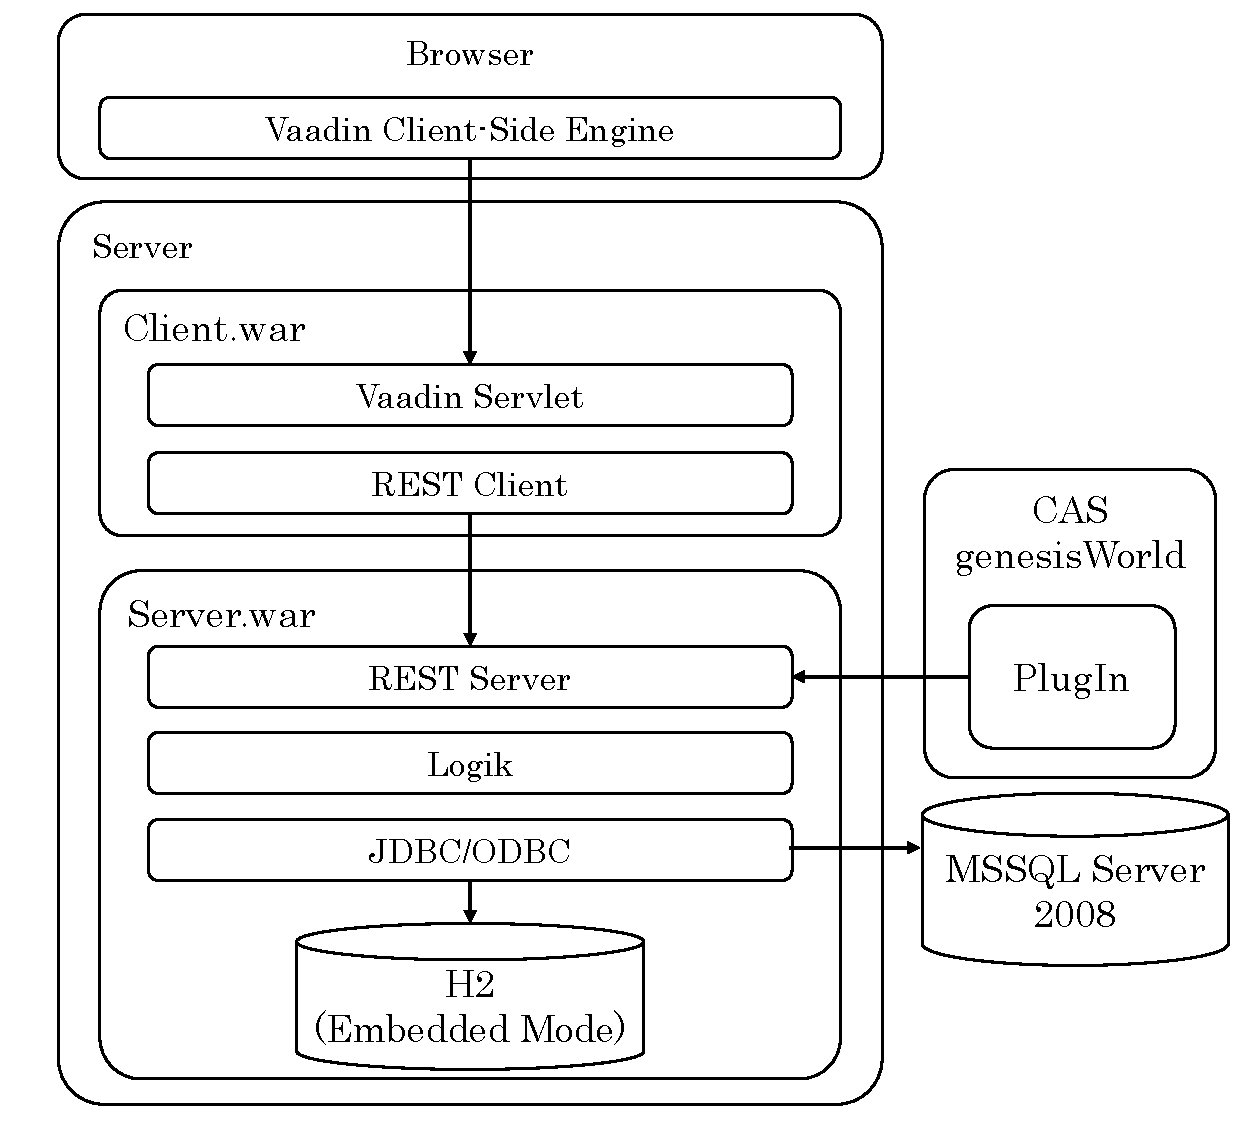
\includegraphics[width=0.8\textwidth, width=0.8\textwidth]{pics/Konzept_architektur.pdf}
\caption{Komponenten des Systems und der Umwelt}
\label{konzept_architektur}
\end{figure} 

\paragraph{Vaadin Client-Side-Engine}

Die Vaadin Client-Side-Engine verwaltet das Rendering der Oberfläche im Web-Browser.  Dies geschieht durch den Einsatz verschiedener clientseitiger Widgets, die das Gegenstück zu den serverseitigen Vaadin-Komponenten bilden. Es leitet Benutzerinteraktionen an die Serverseite weiter und rendert anschließend die Änderungen für die Benutzeroberfläche. Die Kommunikation findet über asynchrone HTTP-oder HTTPS-Anfragen statt. Weiterhin wird die Komponente durch Vaadin automatisch erzeugt und wird daher als gegeben betrachtet.

\paragraph{Client-Webprojekt}

Die Oberfläche des Systems wird durch ein Vaadin-Projekt realisiert. Mit dessen Hilfe werden die Bedien- und Darstellungselemente der Anwendung definiert. Sie ist außerdem für die Interaktion mit dem Benutzer zuständig. Die Delegation von verschiedenen Clients beispielsweise wird von einem Vaadin-Servlet erledigt. Dazu zählt das Empfangen von Anfragen und deren Zuordnung zu einer Sitzung des jeweiligen Benutzers. Die Elemente der Oberfläche selbst werden in Java geschrieben. Mithilfe der Java-Klasssen wird zur Laufzeit eine Javascript basierte Homepage erzeugt. Die Übersetzung von Java auf Javascript übernimmt Vaadin.

Das Server-Webprojekt ist eine weitere Komponente mit der interagiert werden soll. Die Kommunikation zwischen den beiden Komponenten soll über das REST-Protokoll stattfinden. Dazu implementiert das Client-Webprojekt einen REST-Client. Die Verwendung des REST-Protokolls zwischen dem Client-Webprojekt und Server-Webprojekt stellt überdies einen weiteres Element der losen Kopplung dar.

Ein Prozess in dem die einzelnen Bestandteile Verwendung finden, könnte wie folgt aussehen: Die Interaktionen der Benutzer mit der Oberfläche würden Events erzeugen, die zunächst auf der Clientseite durch Widgets verarbeitet werden. Nachfolgend würden die Events durch den HTTP-Server an das Vaadin-Servlet übergeben werden. Dieser leitet die Events an die entsprechenden Vaadin-Objekte weiter, bis sie zu den in der Anwendung definierten Event-Listenern gelangen. In den Listenern werden anschließend die REST-Clients aufgerufen. Mit Hilfe der REST-Clients werden die Eingaben der Nutzer an das Server-Webprojekt übermittelt. 

\paragraph{Server-Webprojekt}

Die eigentliche Lösung der Problemstellung soll im Server-Webprojekt des Softwaresystems implementiert werden. Es soll vollständig auf Java basieren. In ihr werden sich Klassen und Methoden befinden die eine Ermittlung der Informationen aus der H2-Datenbank ermöglichen. Zur Bestimmung der SQL-Parameter soll ein REST-Server implementiert werden, der die Beinutzeingaben entgegennimmt. Der REST-Server ist außerdem für die Kommunikation mit dem Plugin zuständig.

Weiterhin soll das Projekt sämtliche ETL-Prozessschritte implementieren. Die genauen Prozessschritte werden in Abschnitt \ref{ch:konzeption:etl} behandelt. 

%Die Logikkomponente in der Architektur stellt eine Zusammenfassung aller Funktionen des Anwendungskerns dar. Sie kümmert sich um die Generierung der Abfragen, welche an die Datenbank gestellt werden. Dabei erfolgt eine dynamische Generierung der Abfragen, um nicht durch unnötige Bedingungen die Verarbeitungsgeschwindigkeit zu verringern. Abfragen werden mithilfe der Java Database Connectivity (JDBC) an die Datenbank gestellt. Neben den Funktionen zur Abfragegenerierung enthält die Logikkomponente Prozesse zum Extrahieren und Transformieren von Daten aus der MSSQL-Datenbank. Der ETL-Prozess wird nur einmalig ausgeführt, allerdings stellt er einen wichtigen  Schritt für die Umsetzung dar. 


%In der Server.war werden REST-Requests entgegen genommen. Anhand der mitübertragenen Filteroptionen werden die Bedingungen für die Datenbankabfrage zusammengestellt. Anschließend wird eine Verbindung zur H2-Datenbank aufgebaut. Das Ergebnis der Abfrage wird in das JSON-Format überführt und zurück an die Client.war geschickt. Dort angekommen werden die Daten an die Vaadin-Komponenten übergeben, was einen Neuaufbau der entsprechenden Seitenbereiche bewirkt.      

\paragraph{H2-Datenbank}

Die H2-Datenbank ist als ein Bestandteil des Server-Webprojektes geplant. Dies ist durch den Betrieb im Embbeded-Modus möglich. Dadurch kann direkt aus dem Java-Code heraus mit der Datenbank gearbeitet werden. Um möglichst kurze Antwortzeiten zu Erreichen soll die In-Memory-Variante der Tabellen verwendet werden.

\paragraph{CAS genesisWorld Plugin} Systeme die auf dem Datenbestand anderer Systeme aufbauen können zwei verschiedene  Ansätze zur Sicherstellung ihrer Aktualität verfolgen. Unser nebenläufiges System bezeichnen wir als A und den CAS genesisWorld Anwendungsserver als B. Einer der Ansätze ist die Intervall basierte Nachfrage über Veränderungen von A. Hierbei fragt A bei B zu festgelegten Zeitpunkten nach, ob Daten verändert wurden. Die Definition eines optimalen Intervalls stellt eine der größten Schwierigkeiten dar. Ist der Intervall zu groß, sinkt die Aktualität des Datenbestandes. Ist er zu klein, entsteht eine starke Belastung für B. Der andere Ansatz ist A über Veränderungen an den Datensätzen von B zu informieren. Dadurch werden keine unnötigen Abläufe angestoßen, da nur im Falle einer Manipulation eines Datensatzes Prozesse in Bewegung gesetzt werden. Zwar wird die Aktualität der Daten gewährleistet, jedoch büßt A an Entscheidungsfreiheit ein. A kann nicht mehr selbst entscheiden wann aktualisiert wird. Der zweite Ansatz ist zwar effizienter, allerdings nicht immer umsetzbar. Das kann technische oder unternehmenspolitische Gründe haben, die notwendige Veränderung am Legacy-Systems ausschließen.  

In CAS genesisWorld gibt es die Möglichkeit den zweiten Ansatz umzusetzen. Die Idee dabei ist den CAS genesisWorld Anwendungsserver um ein Plugin zu erweitern, welches über Veränderungen in den Datensätzen benachrichtigt wird. Das Plugin soll über einen REST-Client die \textit{GGUID} des betroffenen Datensatzes an den Server-Webprojekt senden. Dort soll eine Kontrolle stattfinden, die den Datensatz auf Relevanz überprüft. Wird eine Relevanz festgestellt besorgt sich das Server-Webprojekt, anhand der zuvor übermittelten GGUID, alle benötigten Daten.

%% ===========================
\section{Datenbankdesign}
%% ===========================

Das Datenbankdesign stellt einen wichtigen Abschnitt in der Konzeption dar. An dieser Stelle werden Festlegungen im Bereich des Datenmodells getroffen. Sie entscheiden, ob Anforderungen und Erwartungen erfüllt werden können. Weiterhin werden die Charakteristika der Daten untersucht und das Datenmodell entsprechend nach ihnen gestaltet.

%% ===========================
\subsection{Konzeptionelles Design}
%% ===========================

Zunächst wird auf das geplante Schema der H2-Datenbank eingegangen. Indessen werden die Überlegungen und Entscheidungen die zur Entstehung des Schemas geführt haben erläutert. 

Die Normalisierung dient der Organisation von Feldern und Tabellen einer relationalen Datenbank, um Redundanz und Abhängigkeit zu minimieren. Die Kehrseite hingegen, ist eine Steigerung des Aufwands, um die benötigten Daten wiederzugewinnen. Normalisierung bietet dem Designer die Möglichkeit einen Austausch zwischen Performance und Stabilität des Datenbankmodells vorzunehmen \cite{geisler2011datenbanken}. Im neuen System stellt ersteres absolute Priorität dar. Daher soll die Normalisierung so gering wie möglich gehalten werden. 

Die erste Überlegung hinsichtlich des Schemas führt zu der Frage, welche Daten zur Umsetzung des Systems beibehalten werden. Der Datenbankdesigner steht bei analytischen System immer wieder vor der Entscheidung, wie viele Informationen aus dem alten System in das neue System übernommen werden sollten. Um höchstmögliche Verarbeitungsgeschwindigkeiten zu erreichen, werden lediglich die für das Szenario benötigten Daten extrahiert. Abbildung \ref{konzept_SchemaNeu} zeigt das für die Datenbank neu entworfene Schema. 

\begin{figure}[htbp]
\centering
  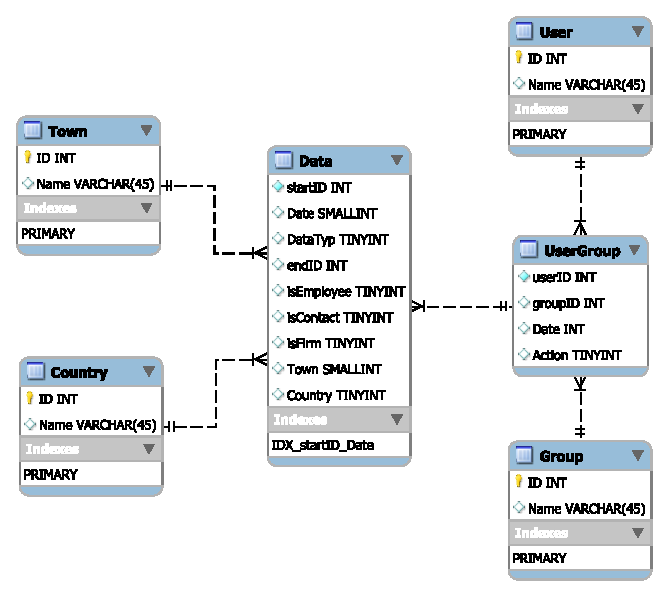
\includegraphics[width=0.8\textwidth, width=0.8\textwidth]{pics/NewSchema.pdf}
\caption{Neues Datenbankschema}
\label{konzept_SchemaNeu}
\end{figure} 

Die Idee hinter dem Schema ist die Verwendung einer einzelnen Tabelle zur Aufbewahrung der Informationen über die CRM-Objekte, die unter Personen geteilt werden. Diese Tabelle ermöglicht es ausgehend von einer Person alle CRM-Objekte die zu anderen Personen führen zu ermitteln. Die ersten vier Spalten werden benötigt, um die Anzahl der CRM-Objekte zwischen Personen festzustellen. Die erste Spalte \textit{startID} beinhaltet die Person von der die Bewertung ausgeht. Eine Zuordnung der Tupel zu einem Datum erfolgt über die Spalte \textit{Date}. Um CRM-Objekte zu unterscheiden, werden Zahlen von eins bis fünf in der Spalte \textit{DataTyp} für die jeweiligen Objekte verwendet. Die letzte Spalte \textit{endID} beinhaltet die ID der Personen mit der das CRM-Objekt geteilt wird. Alle anderen Spalten, wie \textit{Town} oder \textit{Country}, dienen dem Ausschluss von Personen aus der Abfrage.

Um mit den geringeren Speicherkapazitäten des Hauptspeichers zurechtzukommen, wird auf das Problem der Datenredundanz eingegangen. Durch Normalisierung lässt sich Datenredundanz zwar nicht verringern, allerdings kann man sie in kontrollierbare Bahnen lenken. Im neuen Schema werden solche Maßnahmen auf die Spalte \textit{Town} und \textit{Country} angewendet. 

Die Spalte \textit{Country} beispielsweise wird voraussichtlich Millionen von Werten beinhalten, jedoch gibt es im Vergleich nur wenige Länder auf der Welt. Die Ländernamen werden sich daher sehr oft wiederholen. Der Datentyp Varchar benötigt pro Zeichen 2 Byte an Speicherplatz. Aufgrund der stetigen Wiederholung von gleichen Wörtern ist die Verwendung von Varchar an dieser Stelle ungeeignet. Angesichts dessen werden die Ländernamen in einer eigenen Tabelle aufbewahrt. In dieser wird jedes Land nur einmal vermerkt und bekommt einen Primärschlüssel in Form einer Zahl. In der Tabelle \textit{Data} wird dann nur noch der jeweilige Fremdschlüssel verwendet. Das würde zum Beispiel bei dem Wort "Deutschland" eine Reduktion von 22 Byte auf 1 Byte bewirken. Die Reduzierung auf 1 Byte entsteht durch die Verwendung des Datentyps tinyint. Das alles gilt ebenfalls für die Spalte \textit{Town}. Bei ihr wird allerdings der Datentyp smallint verwendet, da dessen Zahlenbereich von -32768 bis 32767 reicht. Damit lassen sich alle Städte aus der MSSQL-Datenbank abdecken. 

Die Spalten \textit{isEmployee}, \textit{isContact} und \textit{isFirm} können nur zwei verschiedene Zustände darstellen. Trifft zu oder trifft nicht zu. Der Datentyp \texttt{bool} reicht daher zur Abbildung der zweiwertigen Zustände aus. Ein Feld vom Datentyp datetime benötigt 8 byte an Speicher. Um hier ebenfalls Einsparungen vorzunehmen, wurde beschlossen das Datum als smallint zu deklarieren. Dies ist möglich, weil nur der Tag des Datums von Interesse ist. Dazu wird ein frei gewählter Nullpunkt festgelegt. In unserem Fall wurde der 01.01.1990 als Nullpunkt gewählt, da keine älteren Daten existieren, die eine Relevanz besitzen. Der Wert eines Datum wird durch die Anzahl der Tage seit dem Nullpunkt ermittelt. Ein Beispiel wäre der 05.01.1990 der in der Spalte als 4 vermerkt werden würde. Die Hochrechnung der Tabelle \ref{tb_speicherplatzverbrauch} zeigt, dass durch die Normalisierung der Speicherplatzverbrauch um bis zu $ \frac{1}{6} $ gesenkt werden kann.

\begin{table}[htbp]
\centering
\begin{tabulary} {\linewidth} {l  r  C  l  C  r}
& & & & & \\
\multicolumn{6}{l}{Speicherplatzverbrauch ohne Normalisierung}\\
& & & & & \\
Zeitpunkt(timestamp) & 8 byte & x & 18.000.000 & = & \textasciitilde 137 MB \\  
Stadt(varchar) & 16 byte & x & 18.000.000 & = & \textasciitilde 343 MB \\  
Land(varchar) & 20 byte & x & 18.000.000 & = & \textasciitilde 274 MB \\  
\midrule
& & & & Summe & \textasciitilde 754 MB\\
& & & & & \\
\multicolumn{6}{l}{Speicherplatzverbrauch mit Normalisierung}\\
& & & & & \\
Zeitpunkt(smallint) & 2 byte & x & 18.000.000 & = & \textasciitilde 34 MB \\  
Stadt(integer) & 4 byte & x & 18.000.000 & = & \textasciitilde 72 MB \\  
Stadt(varchar) & 16 byte & x & 21.000 & = & \textasciitilde 0,32 MB \\  
Land(tinyint) & 1 byte & x & 18.000.000 & = & \textasciitilde 17 MB \\  
Land(varchar) & 20 byte & x & 218 & = & \textasciitilde 0,004 MB \\
\midrule  
& & & & Summe & \textasciitilde 123 MB\\
& & & & & \\
\end{tabulary}
\caption{Vergleich des Speicherplatzverbrauchs}
\label{tb_speicherplatzverbrauch}
\end{table}

Durch die zusätzlichen Tabellen kann zwar Speicherplatz gespart werden doch nun muss überlegt werden wie die Informationen wiederbeschafft werden sollen. Wird eine Benutzerabfrage gestellt die eine Filterung anhand einer Stadt voraussieht, wird zuerst die \textit{ID} der Stadt benötigt. Dabei können zwei verschiedene Ansätze verfolgt werden. Der erste Ansatz wäre ein Verbund zwischen \textit{Town} und \textit{Data}, um direkt mit dem Namen der Stadt zu arbeiten. Diese Variante dürfte aufgrund des Kreuzproduktes von Millionen von Zeilen nicht sehr performant sein. Eine andere Möglichkeit wäre eine separate Abfrage an die Datenbank zu stellen, in der die \textit{ID} zum Namen ermittelt wird. Mithilfe der \textit{ID} kann dann ohne einen Verbund die Ergebnismenge ermittelt werden. Dieser Ansatz dürfte zu geringeren Antwortzeiten führen, da keine Verzögerungen durch Netzwerkzugriffe entstehen. Dieses Vorgehen kann für die Stadt, das Land und die Gruppenzugehörigkeit angewendet werden.

Die Tabelle \textit{GroupDate} unterscheidet sich von den anderen Tabellen wie \textit{Town} oder \textit{Country}, da in dieser noch weitere Details vermerkt sind. Diese ermöglichen es die Zusammenstellung von Gruppen über die Zeit nachzuvollziehen. In der Spalte \textit{Action} wird festgelegt, ob die Tupel einen Eintritt oder einen Austritt einer Person darstellt. Die Spalte \textit{Date} beinhaltet das Datum des Ereignisses. Mithilfe beider Attribute lassen sich Gruppenzusammensetzung auf bestimmte Zeitpunkte bezogen rekonstruieren.

%% ===========================
\subsection{Zugriffsstrukturen}
%% ===========================

Zum Beschleunigen der Zugriffe auf die Datensätze der H2-Datenbank wird auf die beabsichtigten Zugriffsverfahren eingegangen. 

Indizes werden zur Beschleunigung von Suchen nach bestimmten Spaltenwerten eingesetzt. Ohne Indizes müsste die H2-Datenbank beim ersten Datensatz beginnen und dann die gesamte Tabelle durchgehen, um eine Abfrage zu beantworten. Je größer die Tabelle ist, desto höher ist der Aufwand dafür. Der Einsatz von Indizes ist in Anbetracht der Zielsetzung von kurzen Antwortzeiten ein interessantes Hilfsmittel. Jeder Index bedeutet allerdings einen Zuwachs im Speicherplatzverbrauch. Zur Indexierung der Tabellen \textit{Town},\textit{UserGroup}, \textit{Country}, \textit{User} und \textit{Group} eignen sich Hash-Indizes. Sie bieten einen extrem schnellen Zugriff auf die Daten. Diese Schnelligkeit ergibt sich aus der Verwendung von Berechnungsvorschriften, zur Ermittlung der Position des gesuchten Wertes. Indizierungen sollen im vorliegenden Schema über die Spalten mit der Bezeichnung \textit{Name} vorgenommen werden, da der Client mit dem Namen anstatt mit der ID arbeitet. Mithilfe des Namens wird anschließend die zugehörige ID ermittelt. Die Nutzung von Hash-Indizes bringt allerdings Limitierungen mit sich. Eine der wichtigsten ist, dass sie nur für Vergleiche ("=") verwendbar sind. Somit werden keine Wertebereichabfragen ("<" oder ">") unterstützt. Es gibt allerdings noch andere Nachteile \cite{SWB-352401869}, auf die aber in dieser Arbeit nicht näher eingegangen wird. 

Für die Tabelle \textit{Data} eignet sich der B\textsuperscript{+}-Baum-Index. Er ermöglicht eine effizientere Ausführung der Grundoperationen wie Suchen, Einfügen und Löschen. Die Spalte \textit{startID} und \textit{Date} eignen sich am besten für die Indexierung. Dabei handelt es sich um einen Mehr-Attribut-Indexe, da wir zwei Attribute verwenden. Der Vorteil eines Mehr-Attribut-Indexes ist, dass bei einer Punkt-Abfrage über alle Zugriffsattributwerte nur ein Indexzugriff erfolgen muss.
Beide Spalten sind sortiert und bieten sich somit für die Verwendung von einem geclusterten Index an. Ein Geclusterter Index ist in der gleichen Form sortiert wie die interne Relation. Dadurch unterstützt bietet er eine sehr gute Unterstützung für Bereichsabfragen. Dieser Vorteil kann in der Spalte Date ausgenutzt werden, da in den Abfragen immer ein bestimmter Zeitraum betrachtet wird.


%% ===========================
\section{ETL-Prozess}
\label{ch:konzeption:etl}
%% ===========================

Daten der operativen Systeme unterstützen die wertschöpfenden Geschäftsprozesse innerhalb eines Unternehmens. Sie sind demnach auf die Steuerung und Überwachung des Tagesgeschäftes ausgerichtet und daher transaktionsbezogen. Somit sind die Daten in ihren Begrifflichkeiten häufig nicht vergleichbar und ihrer Bewertung sowie Konsolidierung unterschiedlich. Um die Daten dennoch für analytische Zwecke einzusetzen, ist eine Überführung in eine geeignete Struktur von Vorteil. Eine solche Überführung wird in der Literatur als Extract-Transform-Load (ETL)-Prozess bezeichnet \cite{ElSappagh201191}. 

Abbildung \ref{konzept:etl} zeigt das erarbeitete Konzept zur Umsetzung eines solchen ETL-Prozesses. In den nächsten drei Abschnitten wird jeder ETL-Schritt näher erläutert.

\begin{figure}[htbp]
\centering
  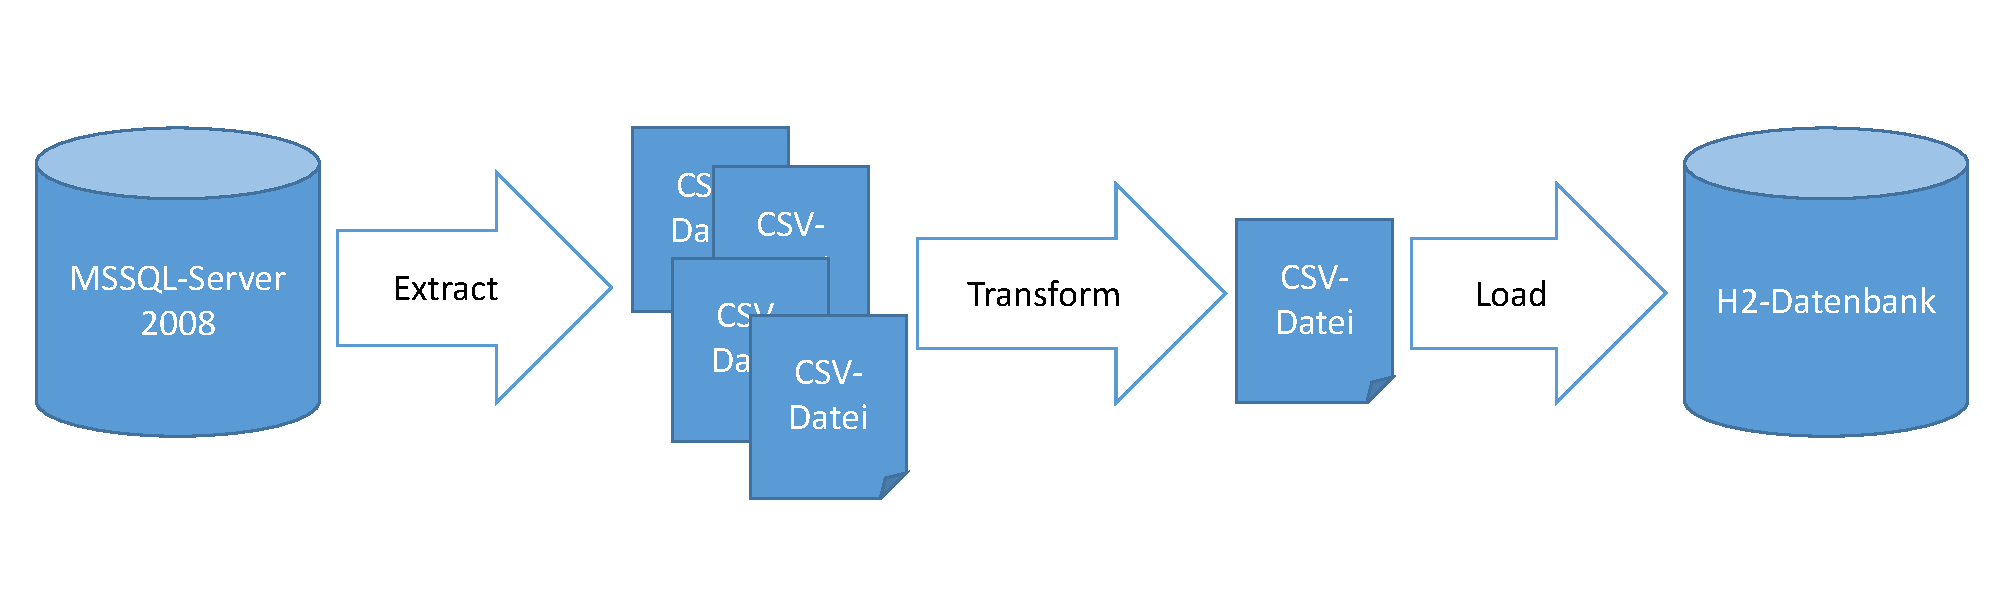
\includegraphics[width=1.0\textwidth, width=1.0\textwidth]{pics/ETL.pdf}
\caption{ETL-Prozess}
\label{konzept:etl}
\end{figure} 


%% ===========================
\subsection{Extract}
\label{ch:konzeption:etl:extract}
%% ===========================

Zunächst dient die Extraktion primär der Beschaffung von Daten aus der MSSQL-Datenbank. Überdies können durch den Prozess Daten bereits reduziert,  zusammengeführt und ersetzt werden. Für eine zutreffende Formulierung der Abfragen müssen Besonderheiten in die Ermittlung der Daten beachtet werden. Eine vollständige und korrekte Datenmenge stellt die Grundlage jeder guten Analyse dar.

In der Extraktion sollen SQL-Abfragen formuliert werden mit denen die Daten aus der MSSQL-Datenbank in die H2-Datenbank überführt werden können. Dabei gilt es die Abfragen so zu formulieren, dass das Ergebnis den Attributen aus der Tabelle des neuen Schemas entspricht.

Weiterhin sind Besonderheiten in der Extraktion zu beachten. Es existieren Datensätze in der MSSQL-Datenbank die sich über längere Zeiträume erstrecken. Beispielsweise erstrecken sich Termine wie Tagungen über mehrere Tage. In der MSSQL-Datenbank werden diese Termine in einer Tupel aufbewahrt. Bei unserer Analyse hingegen stellt jede Tupel eine Verbindung zu einem bestimmten Tag dar. Somit muss ein Datensatz der sich über mehrere Tage erstreckt, in der H2-Datenbank durch mehrere Tupeln repräsentiert werden. Aufgrund dessen wird im Ergebnis der SQL-Abfrage die Zeitspanne eines CRM-Objektes in Tagen vermerkt. In späteren Transformationen kann mithilfe dieser Angaben die entsprechende Anzahl an Tupeln erzeugt werden.

Eine weitere Besonderheit ergibt sich durch eine Funktionalität von CAS genesisWorld, welche es ermöglicht Termine zu schieben. Diese Funktion wird von manchen Nutzern missbraucht. Anstatt für einen ähnlichen Termin einen neuen Eintrag anzulegen, wird ein alter Termin aus Bequemlichkeit geschoben. Das hat zur Folge, dass Termine die tatsächlich stattgefunden haben, in der Datenbank nicht mehr existieren. Um trotzdem diese Termine zu berücksichtigen wurde folgendes Konzept erarbeitet. 

Dem \textit{Changelogbook} lassen sich Veränderungen von Feldern entnehmen. Um Schiebungen zu erkennen werden die Änderungen in den Spalten \textit{start\_dt} und \textit{end\_dt} benötigt. Zur Feststellung ob ein Termin stattgefunden hat und anschließend geschoben wurde, müssen drei Bedienungen erfüllt sein. Die erste ist der Zeitpunkt der Schiebung, der nach dem Termin liegen muss. Wird ein Termin aus anderen Gründen geschoben findet dies in der Regel vor dem Start des Termines statt, damit die Personen nicht unnötig zum Termin erscheinen. Die zweite Bedingung ist, dass der neue Termin in der Zukunft liegen muss. Neben den beiden zuvor genannten Bedingungen muss die Operation auf den Datensätzen ein Update gewesen sein. Nur dann ist der Datensatz von Relevanz für die Ermittlung der geschobenen Termine. 

Die Ergebnisse sämtlicher Extraktionen werden in CSV-Dateien abgespeichert. Damit werden unteranderem eventuelle Fehlersuchen vereinfacht. Weiterhin wird die Belastung des Hauptspeichers verringert, da nicht alle Ergebnisse bis zum Ende der Extraktion in der Java-Laufzeitumgebung aufbewahrt werden müssen.

%% ===========================
\subsection{Transform}
%% ===========================

Zu Beginn der Transformation werden Filterungen durchgeführt. Unter der Filterung von operativen Daten versteht man eine Bereinigung syntaktischer oder inhaltlicher Defekte, der zu übernehmenden Daten. Die MSSQL-Datenbank besteht zu 37\% aus Nullwerten und zu 4\% aus leeren Feldern. Daten die beispielsweise Nullwerte enthalten und für die Ermittlung des Datums benötigt werden, sind für die Analyse nicht zu gebrauchen. Sie können daher im Laufe des Prozesses aus den Daten entfernt werden. Bei den anderen Filteroperationen können Nullwerte vernachlässigt werden, da sie zweckmäßig abdingbar sind.

Der nächste Schritt ist die Harmonisierung der Daten. Unter anderem besitzen die Telefonnummern kein einheitliches Format. Sie wurde manuell von Sachbearbeitern eingetragen. Zur Lösung des Problems werden aller Nummern in ein einheitliches Format gebracht, welches einen automatischen Vergleich ermöglicht. Die CRM-Objekte müssen ebenfalls in eine einheitliche Struktur gebracht werden. Sie besitzen alle die benötigten Informationen, allerdings werden diese unter Unterschiedlichen Bezeichnungen und eventuell in einem anderen Format aufbewahrt.

Die in der Extraktion genannten Besonderheiten werden durch unterschiedliche Datenbankabfragen ermittelt. Dies führt zu vielen separaten Dateien. Zur Nutzung der Daten sind diese zum Abschluss der Transformation zu sortieren und zusammenzuführen. Das Ergebnis wird anschließend in einer CSV-Datei gespeichert, welche die Basis zum Einspielen der Daten in die H2-Datenbank bildet. 

%% ===========================
\subsection{Load}
%% ===========================

Beim Laden der Datensätze in die H2-Datenbank kommt ein sogenannter "bulk load" zum Einsatz. Dieser wird häufig zum Laden von großen Datenmengen aus einer Datei in eine Datenbank eingesetzt. Er ermöglicht ein wesentlich schnelleres einspielen von großen Datenmengen in die Datenbank, gegenüber der Verwendung von INSERT-Operatoren.

%% ===========================
\section{Entwurf der Oberfläche}
\label{ch:Konzeption:sec:Darstellungskonzepte}
%% ===========================

Bei der Konzeption einer Darstellung ist der Detaillierungsgrad von Informationen ein wichtiger Leitfaden. In unserem Fall ist nicht die Eigenschaft eines CRM-Objekts von interessiere, sondern ihr Typ und ihre Häufigkeit. Da keine detaillierten und privaten Informationen zu den CRM-Objekten aufbewahrt werden, kann jeder Benutzer frei wählen von welcher Person die Bewertung ausgehen  soll. Für die Oberfläche bedeutet dies einen Einstiegspunkt in Form eines Fensters in dem der Benutzername einer Person, von dem die Suche ausgehen soll, eingegeben wird. Zusätzlich soll eine Möglichkeit bestehen die IP-Adresse und Portnummer des Servers anzugeben, um den Client auf anderen Rechnern betreiben zu können.

Nach der Anmeldung findet eine Weiterleitung auf die eigentliche Seite statt. Dessen Aufbau ist in Abbildung \ref{konzept_darstellung} zu sehen. Im oberen Bereich auf der Seite sind alle Regler, CheckBoxen und Eingabefelder zur Filterung der Ergebnismenge zu finden. Direkt darunter befindet sich ein Diagramm, welches das Ergebnis der Abfrage visualisieren soll.

\begin{figure}[htbp]
\centering
  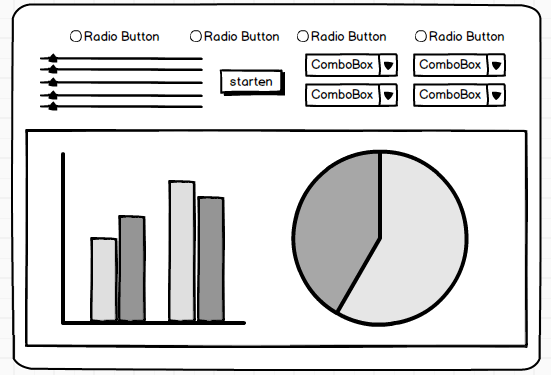
\includegraphics[width=0.8\textwidth, width=0.8\textwidth]{pics/mockup.png}
\caption{Entwurf der Oberfläche}
\label{konzept_darstellung}
\end{figure} 

In der Wahl eines Diagrammtypen ergeben sich allerdings Einschränkungen durch das verwendete Framework. Im Grunde lässt sich jede Darstellung umsetzen, jedoch ist das Aufwand-Nutzen-Verhältnis zu berücksichtigen. In einer Vorauswahl wurden einige  Typen ausgewählt, die in Abbildung \ref{konzept_darstellung2} dargestellt sind. 

Netzdiagramme (a) geben Eigenschaften verschiedener Systeme wieder. Sie eignen sich daher gut zur Darstellung von Ausprägungen. Für die vorliegenden Daten ist diese Darstellung gänzlich ungeeignet, da mit Mengen gearbeitet wird. 

Mithilfe von Liniendiagrammen (b) lassen sich Trends und Zeitreihen darstellen. Die Verwendung verschiedener Linien ermöglicht zudem die Darstellung mehrerer Trends. Die Benutzung dieses Diagramms wäre nicht sinnvoll, da die Ergebnismenge sich nicht auf verschiedene Zeitpunkte bezieht, sondern die Summe der Werte aus einer Zeitreihe beinhaltet. 

\begin{figure}[htbp]
\subfigure[Netzdiagramm]{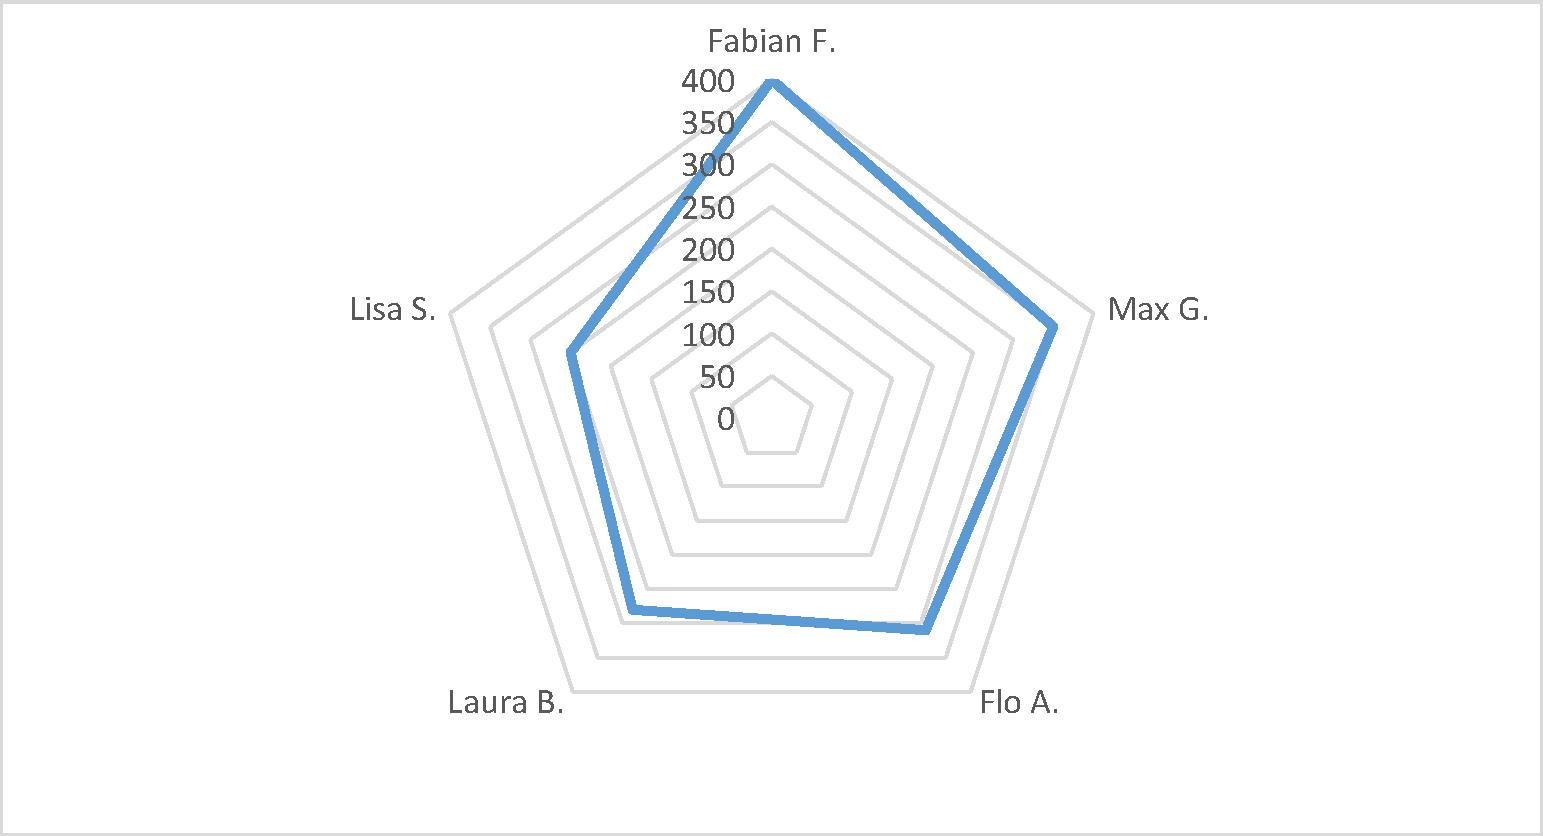
\includegraphics[width=0.3\textwidth]{pics/konzept_netzdiagramm.pdf}}\hfill
\subfigure[Liniendiagramm]{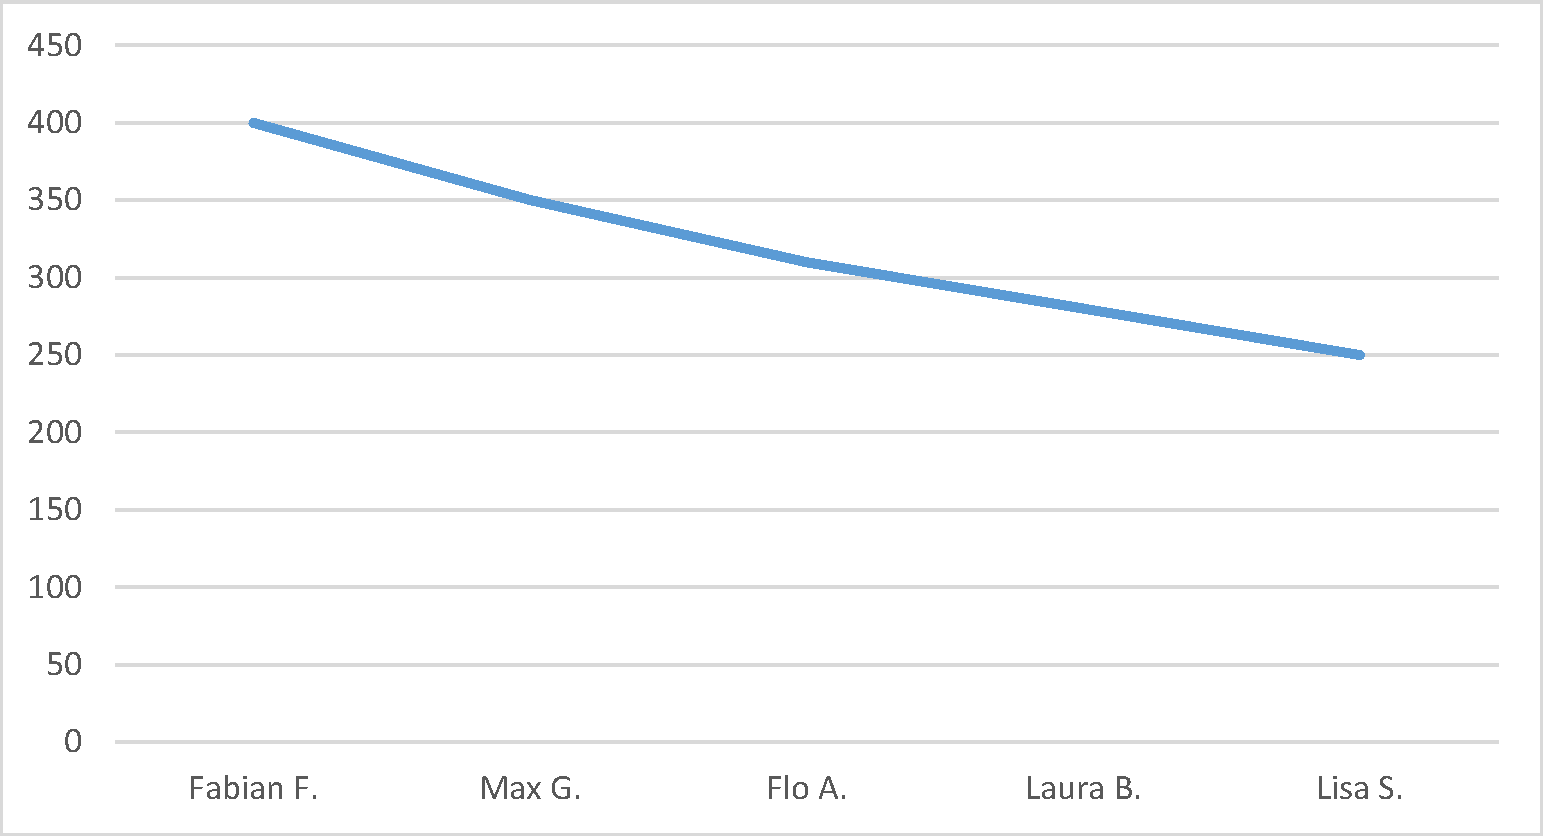
\includegraphics[width=0.3\textwidth]{pics/konzept_liniendiagramm.pdf}}\hfill
\subfigure[Tree Map]{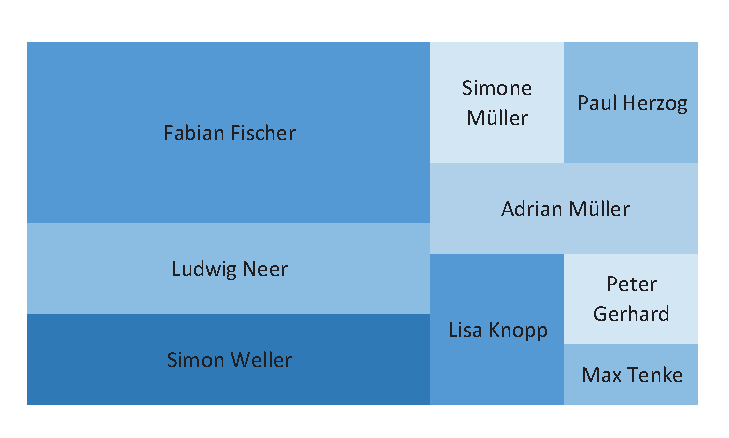
\includegraphics[width=0.3\textwidth]{pics/konzept_tree_map.pdf}}\hfill
\subfigure[Tortendiagramm]{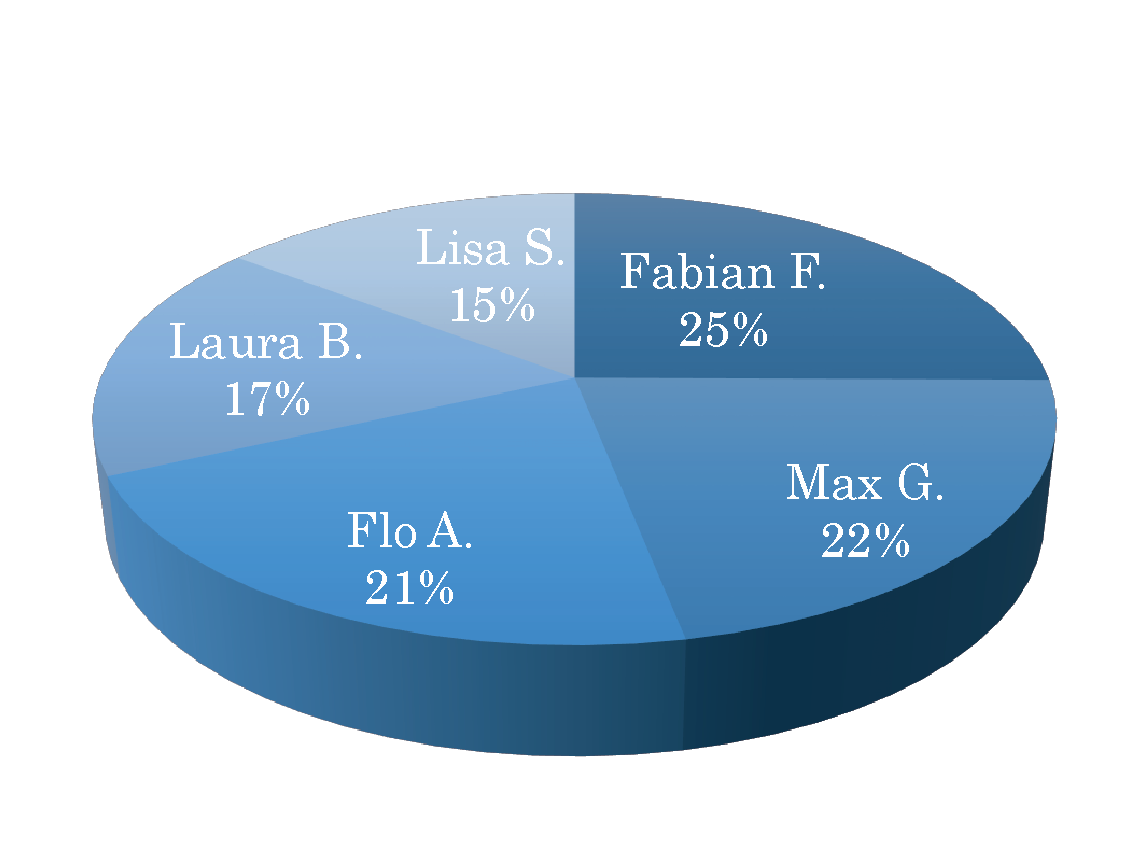
\includegraphics[width=0.3\textwidth]{pics/konzept_tortendiagramm.pdf}}
\subfigure[Balkendiagramm]{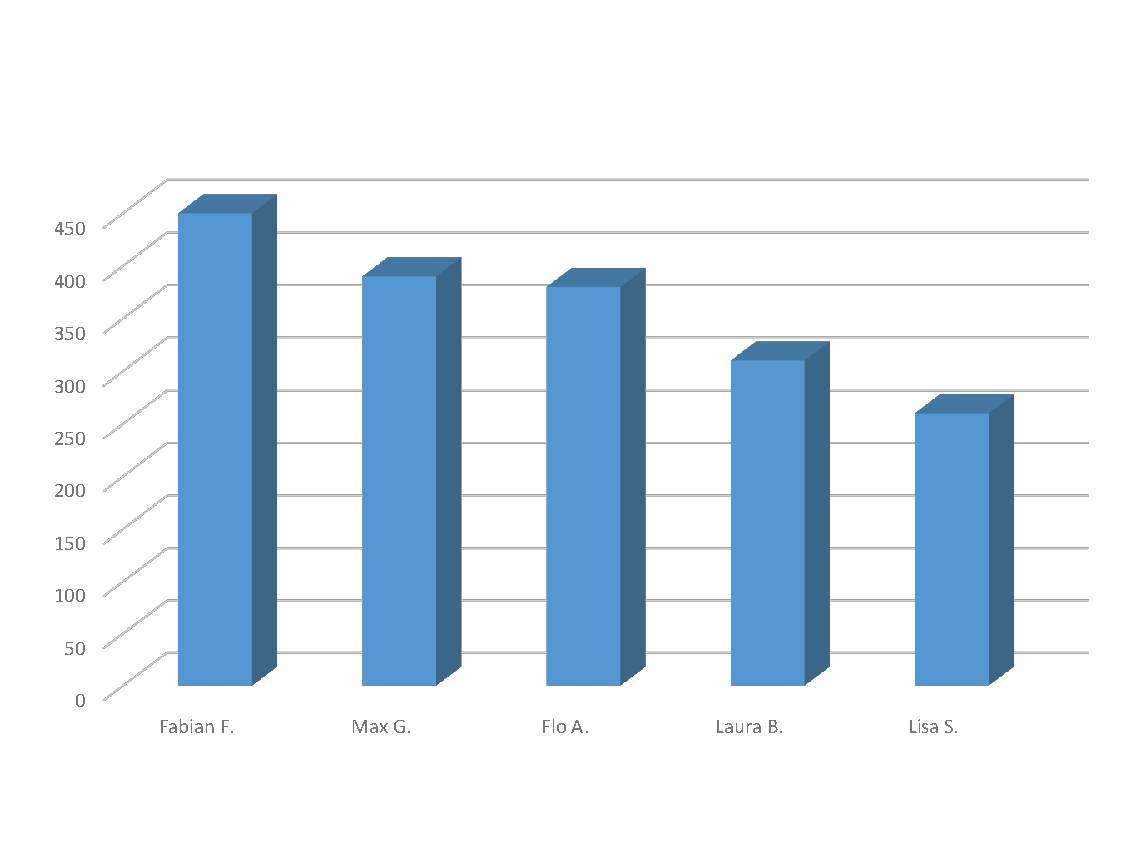
\includegraphics[width=0.3\textwidth]{pics/konzept_balkendiagramm.pdf}}
\caption{Entwürfe für die Oberfläche}
\label{konzept_darstellung2}
\end{figure}

Bei einer Tree Map (c) steht jede Fläche eines Rechtecks im proportionalen Zusammenhang zur Gesamtfläche. Die Beachtung von Größenverhältnissen stellt eine nützliche Eigenschaft für unsere Daten dar. In unserem Fall würde jedes Rechteck aus dem jeweiligen Anteilen der Verbindungsmerkmale bestehen oder mithilfe eines Drilldowns
\footnote{Als Drilldown wird im Allgemeinen die Navigation in hierarchischen Daten bezeichnet. Auf Oberflächen bezogen wird damit die Darstellung von Detailinformationen durch einem Klick auf Darstellungselemente ausgedrückt.}
 die Verbindungsmerkmale aufzeigen. Beispielweise könnte die Person Ludwig Neer wiederum in Rechtecke unterteilt werden, mit der jeweiligen Anzahl der verschiedenen Verbindungsmerkmale. Das würde allerdings aufgrund zu vieler Kacheln schnell zu einer schlechten Übersicht führen. Wird in einer Tree Map die Drilldown-Navigation gewählt, ist die Übersicht aller Informationen auf einen Blick nicht mehr gegeben. Aufgrund der Nachteile in der jeweiligen Variation wurde sich gegen den Einsatz einer Tree Map entschieden.

Kreisdiagramme (d) ermöglichen eine Betrachtung der Gesamtheit zu ihren Einzelstücken, da der Kreis ein geschlossenes System darstellt. Allerdings müssen sich alle Kreisstücke auf die gleiche Basis beziehen. Es eignet sich hervorragend zur Darstellung von Verhältnissen. Wird nun eine weitere Unterteilung der Teilwerte benötigt, geht die Übersicht verloren. Um das zu vermeiden wird die unterteilte Teilmenge häufig in separaten Ansichten dargestellt. Allerdings steigt dadurch der Aufwand für den Nutzer in der Bedienung des Systems. 

Das Balkendiagramm (e) ist für die Darstellung der Daten am geeignetsten. Reihenfolgen beispielsweise lasse sich durch die resultierenden Stufen sehr gut darstellen. Balken selbst lassen sich außerdem in einzelne Teile aufspalten, ohne die Übersichtlichkeit zu verringern. Gegenüber dem Kreisdiagramm kann es zwar keine Betrachtung des Gesamten liefern, allerdings ist das in diesem Anwendungsfall auch nicht nötig. 

%% ===========================
\section{Technologien}
%% ===========================

Als eine der am meist verbreitetsten Programmiersprachen, stellt Java die Grundlage aller verwendeten Technologien dar. Zur Darstellung der Inhalte für den Client wird Vaadin verwendet. Der Apache Tomcat nimmt die Rolle des Anwendungsservers ein. Die Kommunikation auf Basis von RESTful Web Services wird mithilfe von Jersey realisiert. Weiterhin wird opencsv für das Lesen und Schreiben von CSV-Dateien verwendet. JDBC wird zur Kommunikation zwischen dem Anwendungsserver und der Datenbank. Die H2-Datenbank stellt die Datenquelle des Systems dar. Im Folgenden werden alle Bestandteile, bis auf die bereits erläutert H2-Datenbank, näher beschrieben. 

\paragraph{Vaadin}

Vaadin ist ein Open-Source-Framework für den Aufbau von modernen Web-Anwendungen.
Es verwendet ein reines serverseitiges, eventbasiertes Modell und ermöglicht eine Anwendungsentwicklung ohne direkte Verwendung von HTML und JavaScript-Code. Das Framework ermöglicht es, die gesamte Anwendungslogik auf der Serverseite einer Anwendung auszuführen, während die Clientseite nur für das Senden der Benutzeraktionen an den Server und für die Reaktion auf die Antworten verantwortlich ist. Da es auf GWT basiert, kann sowohl der Client- als auch der Server-Code in reinem Java geschrieben werden.

Die aktuelle Version von Vaadin wurde im Februar 2013 veröffentlicht. Die folgenreichste Änderung von Vaadin6 war die Integration von GWT zu Vaadin, die eine bessere Unterstützung für die clientseitige Widget-Entwicklung bedeutet und sogar die Möglichkeit zum Erstellen von Offline-Anwendungen mit sich bringt.

Die im Unternehmen vorhandene Erfahrung und Open-Source stellen relevante Entscheidungsfaktoren in der Wahl von Vaadin. Allerdings war VaadinCharts, eine Erweiterung für Vaadin, für die Auswahl ausschlaggebend. Es basiert auf Highcharts, einem JavaScript-Packet. Highcharts zeichnet sich durch eine umfangreiche Sammlung an Funktionen zur Darstellung von Diagrammen aus. 

\paragraph{Jersey}

Jersey ist ein Open-Source-Framework zur Entwicklung von RESTful Web Services in Java, welches eine Unterstützung für JAX-RS-APIs bietet und die JAX-RS (JSR 311 und JSR 339)-Referenzimplementierung darstellt. JAX-RS-Annotationen werden verwendet um die Relevanz von Java-Klassen für REST zu definieren. Jersey enthält einen REST-Server und einen REST-Client. Auf der Serverseite verwendet Jersey ein Servlet zum Abtasten von vordefinierten Klassen, um REST-Ressourcen zu identifizieren. Über die web.xml Konfigurationsdatei werden die von der Jersey-Distribution bereitgestellten Servlets registriert. Diese Servlets analysieren die eingehenden HTTP-Nachrichten und wählen die richtige Klasse und Methode für die Anfragen aus. Diese Auswahl basiert auf Annotationen in diesen Klassen und Methoden. Weiterhin unterstützt JAX-RS die Erstellung von XML und JSON mithilfe der Java Architektur für XML Binding (JAXB).

\paragraph{Apache Tomcat7}

Tomcat ist ein Open-Source-Webserver, der von der Apache Group entwickelt wurde. Der Apache Tomcat implementiert die Java Servlets-, sowie die JavaServer Pages-Spezifikation von Sun Microsystems und stellt folglich eine Referenzimplementierung dar. Er stellt weiterhin eine rein auf Java-basierende HTTP-Webserverumgebung dar. Weiterhin kann der Tomcat über eine Oberfläche sowie durch Bearbeiten von XML-Dateien konfiguriert werden.

\paragraph{opencsv}

Da Java das Parsen von CSV-Dateien nativ nicht unterstützt, wird auf eine Drittanbieterbibliothek zurückgegriffen. Diese heißt opencsv und ist eine sehr einfache CSV-Parser-Bibliothek für Java. Die Bibliothek kann zum Erstellen, Lesen und Schreiben von CSV-Dateien verwendet werden. Die wichtigste Fähigkeit des opencsv-Parsers ist das Mapping von CSV-Daten auf Java-Bean-Objekte.

\paragraph{JDBC}

Die JDBC-API ermöglicht den programmgesteuerten Zugriff auf relationale Daten, direkt aus der Java Programmiersprache heraus. Durch die Verwendung der JDBC-API können Java-Anwendungen SQL-Anweisungen ausführen, Ergebnisse abrufen und die Veränderungen auf die Datenquelle zurückschreiben. Die JDBC-API kann auch mit mehreren Datenquellen in einer verteilten, heterogenen Umgebung interagieren. 

%% content.tex
%%


%% ===========================
\chapter{Umsetzung}
\label{ch:umsetzung}
%% ===========================

In diesem Kapitel wird auf die Implementierung der Konzepte eingegangen. Die Komponenten des Systems selbst wurden aus architektonischer Sicht, wie in der Konzeption beschrieben umgesetzt. Daher wird vielmehr auf die genaue Umsetzung der Funktionen und Prozesse eingegangen. Anhand von Klassendiagrammen wird in den ersten beiden Kapiteln die Struktur und Funktionsweise der Webprojekte erläutert. Weiterhin wird der ETL-Prozess und die Abfrageerzeugung genauer eingegangen. Der genaue Ablauf in der Aktualisierung wird in dem darauf folgenden Abschnitt beschrieben. Abschließend wird der Aufbau der Oberfläche mit den damit verbundenen Designentscheidungen erläutert. 

%% ===========================
\section{Server-Webprojekt}
%% ===========================

Das Webprojekt behält die Struktur und Einstellungen die beim Erzeugen des Projektes vorgegeben werden bei. Deshalb wird direkt auf die Klassen eingegangen. Abbildung \ref{umsetzung_klassendiagramm_server} zeigt das Klassendiagramm des Server-Webprojekt. Das Diagramm dient als Basis für die nachfolgenden Erläuterungen. 

Die H2-Datenbank wird im Embedded-Modus betrieben, was eine Instanziierung der Datenbank zur Laufzeit notwendig macht. Die Instanziierung erfolgt in der Klasse \textit{Database}. Das Attribut \textit{dataSource} stellt die H2-Datenbank in Form eines Objektes dar. Eine Verbindung zur Datenbank wird mithilfe der Methode \textit{getConnection()} aufgebaut. Diese Verbindung wird permanent offen gehalten, solang der Tomcat-Server läuft. Dazu wird die Verbindung dem Attribut \textit{con} zugewiesen, welches von allen Methoden verwendet wird, die eine Verbindung zur Datenbank aufbauen wollen. Um die Datenbank mit der Web-Anwendungen zu starten, ist die Verwendung eines Servlets nötig. Dazu benutzen wir die Klasse \textit{EntryPoint}, die das Interface \textit{HttpServlet} implementiert. Um das Servlet direkt beim Start aufzurufen sind in der \textit{web.xml} folgende Zeilen eingetragen: 

\begin{lstlisting}[language=XML]
	<servlet>
		<servlet-name>H2</servlet-name>
		<servlet-class>de.cas.db.EntryPoint</servlet-class>
		<load-on-startup>1</load-on-startup>
	</servlet>
\end{lstlisting}

Die 1 im Element \textit{<load-on-startup>} bewirkt den Aufruf der Methode \textit{init()} die eine Instanziierung der Klasse \textit{Database} vornimmt. Zur Erzeugung des Schemas wird eine separate Klasse namens \textit{SchemaBuilder} eingesetzt. In ihr werden sämtliche SQL-Anweisungen zur Generierung des Schemas aufbewahrt und können über die Methode \textit{createSchema()} ausgeführt werden.

\begin{figure}[htbp]
\begin{center}
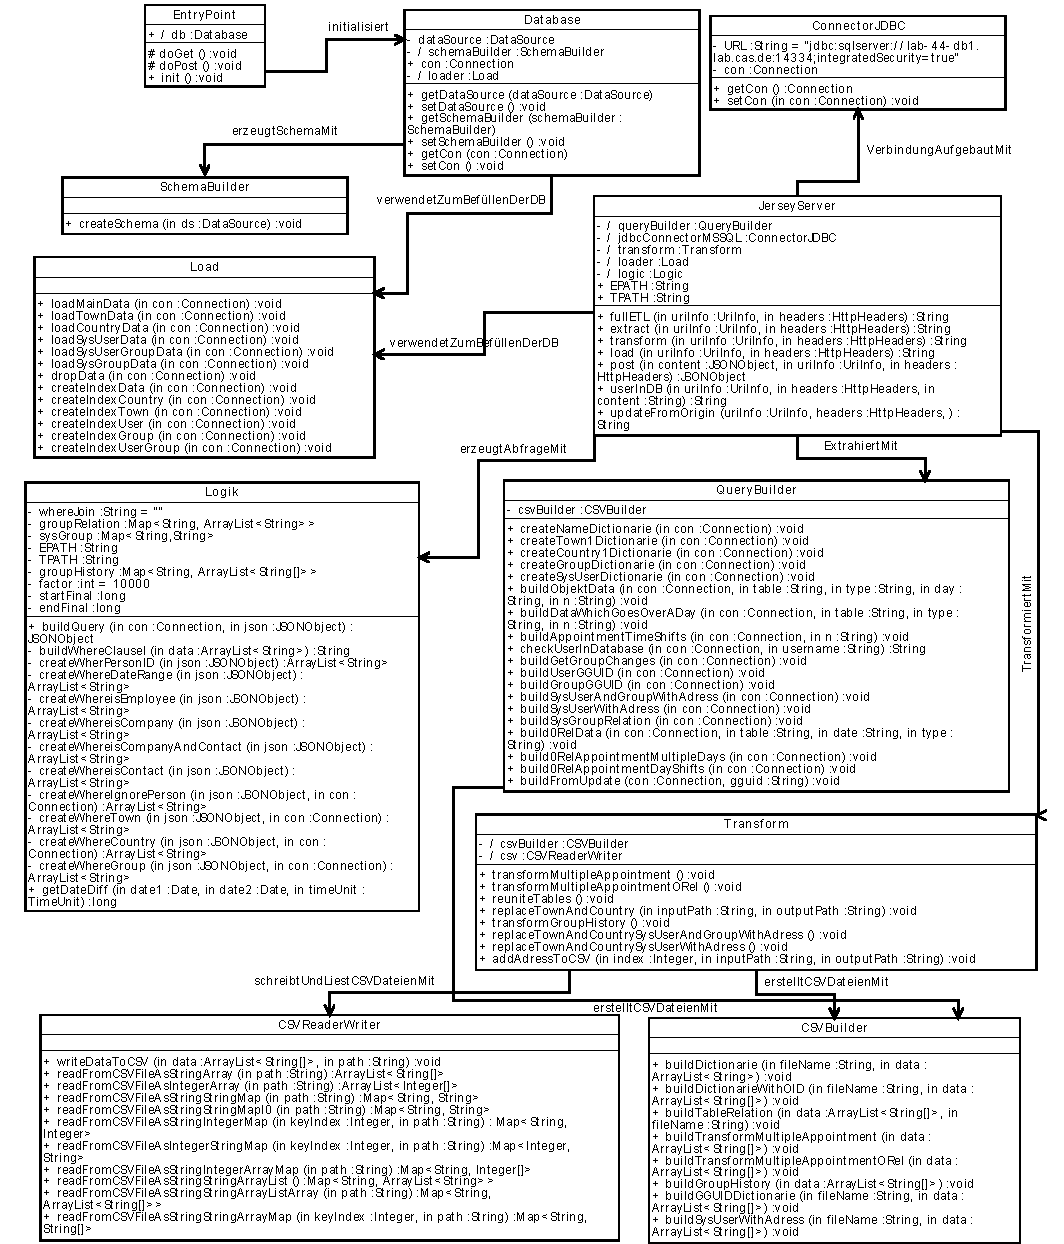
\includegraphics[width=1.0\textwidth]{pics/ServerKlassendiagramm.pdf}
\caption{Server Klassendiagramm}
\label{umsetzung_klassendiagramm_server}
\end{center}
\end{figure}

Mit der Klasse \textit{JerseyServer} wird der REST-Server umgesetzt. Sie besitzt Methoden die mit den entsprechenden Annotationen, wie \textit{@GET} oder \textit{@POST}, die REST-Requests entgegen nehmen. Mit der Annotation \textit{@Path} wird die URL angegeben, unter der die Methode angesprochen werden kann. Diese Methoden können Übergabeparameter vom Typ \textit{UriInfo} und/oder \textit{HttpHeaders} besitzen, die Abrufe von Metadaten der REST-Requests ermöglichen. 

Neben den Methoden zur Beantwortung von REST-Requests, enthält die Klasse alle Objekte zur Durchführung des ETL-Prozesses. Die Klasse \textit{ConnectorJDBC} besitzt ein Attribut namens \textit{con}, welches den Verbindungsaufbau zum MSSQL-Server, mithilfe von JDBC ermöglicht. Zur Extraktion der Daten aus dem MSSQL-Server wird ein Objekt der Klasse \textit{QueryBuilder} verwendet. Wie in der Abbildung zu sehen werden für die verschiedenen Tabellen, des neuen Schemas, eigene Methoden zur Verfügung gestellt. Methoden welche die Übergabewerte \textit{table}, \textit{date} und \textit{n} besitzen, werden für die verschiedenen CRM-Objekte benötigt. Mithilfe des Parameters table wird der Name der Tabelle in der MSSQL Datenbank übergeben. Der Parameter \textit{date} gibt das Feld an, was für die Ermittlung des Datums verwendet werden soll. Um den Typ eines CRM-Objektes zwischen Personen festzuhalten wird der Parameter \textit{n} verwendet, der eine Zahl zwischen eins und fünf beinhaltet. \textit{QueryBuilder} verwendet ein Objekt vom Typ \textit{CSV-Builder}, um die Ergebnisse in Dateien festzuhalten. Den Methoden wird als Übergabeparameter ein Dateiname, sowie die zu speichernden Informationen übergeben.

Die Klasse \textit{Transform} enthält Attribute und Methoden zur Bearbeitung der CSV-Dateien. Weiterhin werden die durch die Extraktionen gewonnen CSV-Dateien mithilfe eines \textit{CSVReaderWriter} Objekts ausgelesen. Nach der Bearbeitung durch die Methoden der \textit{Transform} Klasse, werden die Daten wieder in CSV-Dateien abgelegt. \textit{CSVBuilder} besitzt Methoden die zusätzliche Parameter zum schreiben aufweisen, die modifizierte Schreiboperationen erlauben. Wohingegen \textit{CSVReaderWriter} mithilfe der Methode \textit{writeDataToCSV()}, sowie den Parametern \textit{path} und \textit{data} allgemeine Schreiboperationen durchführt.

Mithilfe der Klasse \textit{Load} wird die Datenbank befüllt. Sie kann wie zuvor erwähnt von einem \textit{Database} Objekt verwendet werden oder durch ein \textit{JerseyServer} Objekt. Beim \textit{JerseyServer} werden mit der Methode \textit{load()} die Methoden der \textit{Load} Klasse aufgerufen. In der Klasse \textit{Database} werden sie im Konstruktor selbst aufgerufen. 

Die Klasse \textit{Logik} beinhaltet Attribute und Methoden zum beantworten von Benutzerabfragen. Um Bedingungen zu einer SQL-Abfrage hinzuzufügen werden separate Methoden verwendet. Die jeweiligen Methoden werden nur gerufen, sobald die entsprechende Bedingung in der vom Nutzer erhaltenen JSON-Datei vorhanden ist. Generiert werden die Abfragen durch die Methode \textit{buildQuery()}. 

%% ===========================
\section{Client-Webprojekt}
\label{ch:Umsetzung:sec:clientwar}
%% ===========================

Einstiegspunkt in der Client.war ist die Klasse \textit{CasAnalyticUI}. Sie ist von der Klasse \textit{UI} abgeleitet. Die \textit{UI} ist die oberste Komponente jeder Komponentenhierarchie in Vaadin. Es gibt eine Benutzeroberfläche für jede Vaadin-Instanz in einem Browserfenster. Ein \textit{UI} Objekt kann entweder ein gesamtes Browserfenster(oder Tab) oder einen Teil einer HTML-Seite, wo eine Vaadin-Anwendung eingebettet ist darstellen. Nachdem eine \textit{UI} von der Anwendung erstellt wurde, wird diese mit der Methode \textit{init(VaadinRequest)} initialisiert. Zur Übersicht werden die Komponenten der Darstellung in die Klasse \textit{RootUI} ausgelagert. 

\textit{RootUI} wird dabei von der \textit{CasAnalayticUI} instanziiert. Die Klasse \textit{RootUI} beinhaltet das Anmeldefenster, sowie die Hauptansicht. Mithilfe der Methode buildLoginView() werden die Komponenten des Anmeldefensters zur \textit{UI} Komponente hinzugefügt. Nach der Erzeugung der Komponenten, wird eine \textit{JerseyClient} Klasse instanziiert. Diese wird verwendet sobald der Nutzer IP, Port und einen Namen eingegeben hat und auf anmelden klickt. Anschließend wird die Methode \textit{doPostRequestUserData()} gerufen, um zu überprüfen ob der Nutzer im System vorhanden ist. 


Falls ja, werden durch die Methode \textit{MainView()} alle bisherigen Komponenten der \textit{UI} entfernt und durch Komponenten des Hauptfensters ersetzt. Das \textit{JerseyClient} Objekt wird direkt im Anschluss verwendet, um Mithilfe der Methode \textit{doPostRequestData()} einen REST-Request an den Server zu senden. Dieser liefert das Ergebnis der Abfrage in einem JSON-Objekt zurück. Mit dessen eine erste Erzeugung des Diagramms durchgeführt wird. Das Diagramm selbst besitzt eine eigene Klasse namens \textit{ChartComponent}. Sie leitet sich von der Klasse \textit{Chart} ab, die Teil der VaadinChart-Bibliothek ist. Mithilfe der Methode \textit{refreshChart()} wird das Diagramm bei Benutzerabfragen aktualisiert. Dazu werden ihr die Namen der Personen für die x-Achse übergeben, sowie die neuen Balkenwerte. Weiterhin wird für jedes Vaadin-Objekt eine separate Methode zur Erzeugung verwendet. Jedes dieser Vaadin-Objekt stellt ein Element an der Oberfläche dar. Änderungen am Aussehen oder an der Funktionalität der jeweiligen Vaadin-Objekte, werden nur innerhalb der entsprechenden Methode vorgenommen.

\begin{figure}[htbp]
\begin{center}
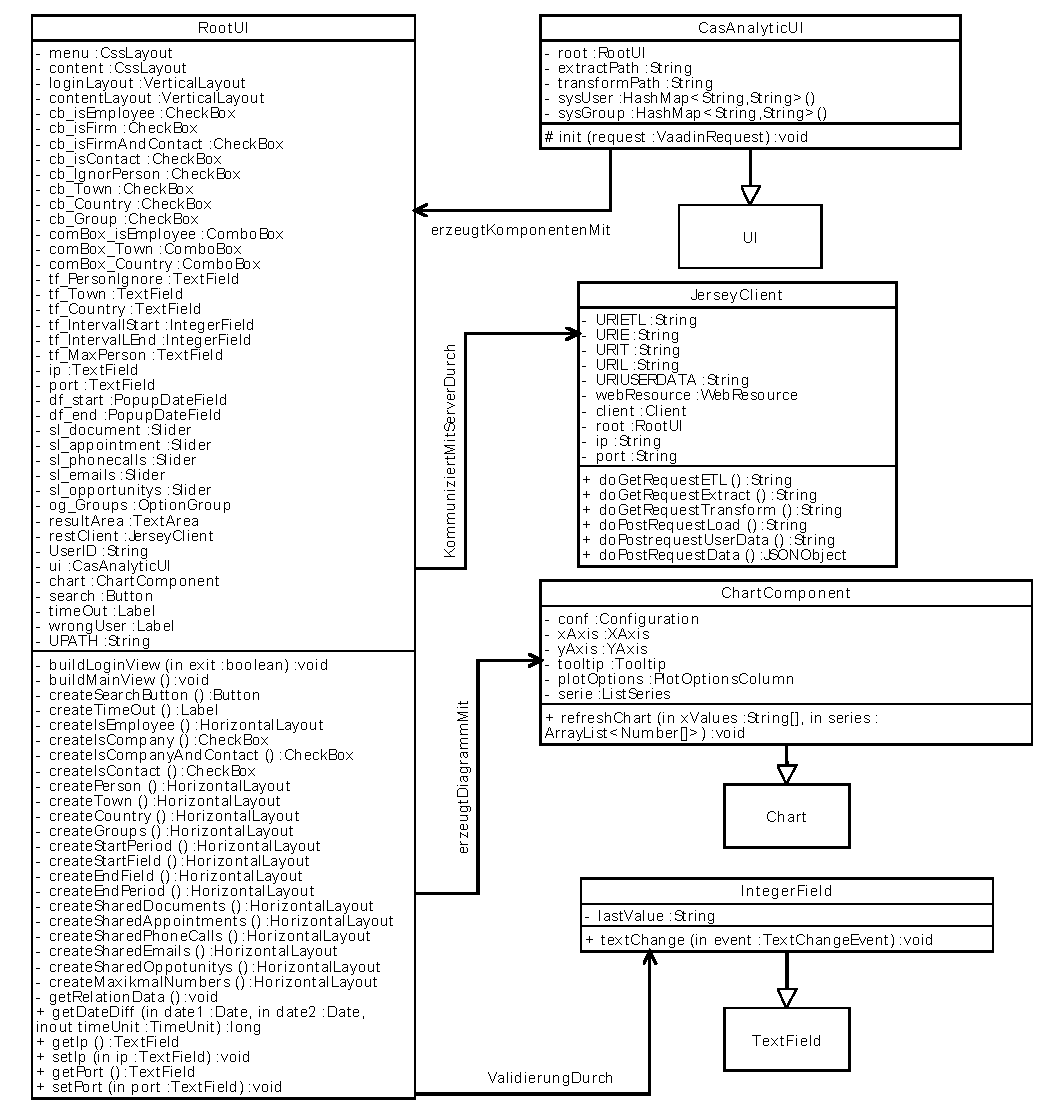
\includegraphics[width=0.9\textwidth]{pics/ClientKlassendiagramm.pdf}
\caption{Client Klassendiagramm}
\label{umsetzung_klassendiagramm_client}
\end{center}
\end{figure}

An der Oberfläche gibt es Felder die nur Zahlen erwarten. Eingaben die nicht numerisch sind werden durch den Einsatz der Klasse \textit{IntegerField} verhindert. Diese erweitert die Klasse \textit{TextField}. Sie besitzt einen Event-Listener, der jede Eingabe des Benutzers abfängt. Gibt der Nutzer nicht numerische Zeichen ein werden diese direkt wieder entfernt. Dadurch werden Falscheingaben durch den Nutzer ausgeschlossen.

%% ===========================
\section{Erzeugung der SQL-Abfrage}
%% ===========================

Um eine SQL-Abfragen mit möglichst wenigen Bedienungen zu verwenden erfolgt die Erzeugung dynamisch. Die SQL-Abfrage kann dadurch je nach Benutzereingabe unterschiedlich aufgebaut sein kann. Die Basisfunktionalität ändert sich allerdings nicht. Diese besteht aus der Bildung von Summen der verschiedenen CRM-Objekte. Nachdem festgestellt wurde wie viele CRM-Objekte von den jeweiligen Typen zu einer Person verlaufen, wird zusätzlich die Gesamtsumme der CRM-Objekte zu einer Person gebildet. Die Summe wird zur Sortierung der Ergebnisse verwendet. Bei der Sortierung wird absteigend vorgegangen, um die Personen mit den meisten CRM-Objekten zu der von der Suche ausgehend Person zu ermitteln. Das Ergebnis wird wiederum auf eine durch den Benutzer festgelegte Anzahl reduziert. Überdies beschränkt die Abfrage den Zeitraum durch die Verwendung der Spalte \textit{Date}.

Nutzer können durch nutzen der Filteroperatoren weitere Bedingungen zur SQL-Abfrage hinzufügen. Eine von ihnen ist die Gewichtung von Zeitspannen. Das Verfahren zur Gewichtung der Zeit wird anhand der Abbildung \ref{fig:umsetzung:gewichtungderzeit} erläutert. Die Abbildung zeigt ein Koordinatensystem mit der Gewichtung von einzelnen Zeitpunkten. Die x-Achse stellt den zeitlichen Verlauf und die y-Achse die Gewichtung dar. Der Startzeitpunkt wird durch $t_{s}$ markiert, wohingegen $t_{e}$ den Endzeitpunkt angibt. Mithilfe von $t_1$ und $t_2$ werden die zu gewichtenden Zeitspannen festgelegt. Um nun die Zeitspannen anders zu gewichten wird eine lineare Abstufung der Tage vorgenommen. Für die Zeitspanne zwischen $t_{s}$ und $t_1$ bedeutet dies, dass der Wert eines Tages zunehmend steigt. Wird $t_1$ erreicht, besitzt jeder Tage wieder eine Wertigkeit von 1. Bei $t_2$ verhält es sich ähnlich. Mit jedem Tag ab $t_2$ sinkt der Wert des Tages bis der Zeitpunkt $t_{e}$ erreicht ist.

Um die Gewichtung eines bestimmten Tages zu berechnen werden die folgenden zwei Faktoren verwendet:

\begin{equation}
f_1 = \frac{1}{t_1 - t_{s}}
\end{equation}
\begin{equation}
f_2 = \frac{1}{t_{e} - t_2}
\end{equation}

Neben den Faktoren $f_1$ und $f_2$ werden Variablen zum erfassen der schrittweisen Erhöhungen und Verringerungen von Tagen benötigt. Für den Zeitraum zwischen   
$t_{s}$ und $t_{1}$ wird die Variable $v_{1}$ verwendet. Im anderen Zeitraum wird die Variable $v_{2}$ benutzt. Die Variable $v_{1}$ beginnt mit dem Wert 0 und erhöht sich mit jedem Tag um 1. Die Differenz zwischen $t_{2}$ und $t_{e}$ stellt den Wert von $v_{2}$ dar. Dieser wird mit jedem Tag ab $t_{2}$ um 1 verringert.

Mit den Faktoren und Variablen werden die Werte der Tage berechnet. Dazu wird der Faktor mit der Variabel multipliziert. Das Produkt bildet den Wert eines Tages. Dieser wird in der Datenbankabfrage verwendet, um Tupeln einen geringeren Wert zuzuweisen. 

\begin{figure}[htbp]
\begin{center}
\begin{tikzpicture}[domain=-1:2] \draw[very thin,color=gray] (0,0); 
\draw[->] (0,0) -- (12.3,0) node[right] {Zeit}; 
\draw[->] (0,0) -- (0,4.2) node[above] {Gewichtung}; 
\draw[color=black]  (0.2,3) -- (-0.2,3)   node[left] {100\%};
\draw[color=black]  (0.2,1.5) -- (-0.2,1.5)   node[left] {50\%};  
%\draw[dashed][color=black]  (4,0.5) -- (4,3.5); 
%\draw[dashed][color=black]  (9,0.5) -- (9,3.5);

\draw[color=black]  (0,0) -- (0,0)   node[below] {$t_{s}$}; 
\draw[color=black]  (4,0.1) -- (4,-0.1)   node[below] {$t_1$}; 
\draw[color=black]  (9,0.1) -- (9,-0.1)   node[below] {$t_2$};
\draw[color=black]  (12,0.1) -- (12,-0.1)   node[below] {$t_{e}$};   
 
\draw[color=black]  (0,0) -- (4,3)   node[right] {}; 
\draw[color=black]  (4,3) -- (9,3)   node[right] {}; 
\draw[color=black]  (9,3) -- (12,0)   node[right] {};  

\draw[dotted][color=black]  (1,0.75) -- (2,0.75);
\draw[dotted][color=black]  (2,1.5) -- (3,1.5);
\draw[dotted][color=black]  (3,2.25) -- (4,2.25);
\draw[dotted][color=black]  (4,3) -- (5,3);

\draw[dotted][color=black]  (1,0.75) -- (1,0);
\draw[dotted][color=black]  (2,1.5) -- (2,0);
\draw[dotted][color=black]  (3,2.25) -- (3,0);
\draw[dotted][color=black]  (4,3) -- (4,0);
\draw[dotted][color=black]  (5,3) -- (5,0);
\draw[dotted][color=black]  (6,3) -- (6,0);
\draw[dotted][color=black]  (7,3) -- (7,0);

\draw[dotted][color=black]  (8,3) -- (8,0);
\draw[dotted][color=black]  (9,3) -- (9,0);
\draw[dotted][color=black]  (10,2) -- (10,0);
\draw[dotted][color=black]  (11,1) -- (11,0);

\draw[dotted][color=black]  (8,3) -- (9,3);
\draw[dotted][color=black]  (9,2) -- (10,2);
\draw[dotted][color=black]  (10,1) -- (11,1);

\draw[dashed][color=black]  (1,0.75) -- (1,1.05)   node[above] {$t_{s}+1$}; 
\draw[dashed][color=black]  (2,1.5) -- (2,1.8)   node[above] {$t_{s}+2$}; 
\draw[dashed][color=black]  (3,2.25) -- (3,2.55)   node[above] {$t_{s}+3$};  

\draw[dashed][color=black]  (10,2) -- (10,2.3)   node[above] {$t_{e}-2$}; 
\draw[dashed][color=black]  (11,1) -- (11,1.3)   node[above] {$t_{e}-1$}; 

\end{tikzpicture} 
\end{center}
\caption{Gewichtung der Zeit}
\label{fig:umsetzung:gewichtungderzeit}
\end{figure}

Neben der Gewichtung der Zeit lassen sich die jeweiligen Verbindungsmerkmale unterschiedlich gewichten. Bei einer Abweichung von 100 Prozent wird die Summe des jeweiligen Verbindungsmerkmales, um die durch den Nutzer bestimmten Prozentsatz verringert. 

Die restlichen Parameter filtern die SQL-Abfrage und werden nach Bedarf hinzugezogen. Eine der Konditionen muss zuvor ermittelt werden und wird daher näher beschrieben. Es handelt sich dabei um Gruppen, die aus der Ergebnismenge ausgeschlossen werden können. Ihre Struktur ist im Laufe der Zeit variabel. Um dies zu berücksichtigen wird die Tabelle \textit{UserGroup} verwendet. Dabei folgendermaßen vorgegangen: Zuerst wird die Ergebnismenge durch die ausgewählten Gruppen reduziert. Anschließend wird für jede Gruppe ein eigener Container erzeugt. Der Container beinhaltet die ID der Personen aus der Gruppe. Liegt nun der Zeitpunkt des Feldes \textit{Date} nach dem Anfangszeitpunkt der Abfrage und die Spalte \textit{Action} enthält eine 1, wird der Container um diese Person reduziert. Enthält sie eine 0, wird die Person zum Container hinzugefügt. Mit einer 1 in der Spalte \textit{Action} wird der Austritt einer Person aus der Gruppe markiert. Eine 0 weist auf den Eintritt einer Person in die Gruppe hin. Dadurch wird die Struktur der Gruppe zum Anfangszeitpunkt wiederhergestellt. Mithilfe der Personen aus den Container, wird nun die SQL-Abfrage um weitere Bedingungen erweitert.

Innerhalb von Zeiträumen können sich Gruppen verändern, jedoch können diese nicht berücksichtigt werden. Es kann jeweils nur ein bestimmter Zeitpunkt betrachtet werden. In unserem Fall entschied man sich für den Anfangszeitpunkt $t_{s}$.

%% ===========================
\section{ETL Prozess}
%% ===========================

Um an die notwendigen Daten zu gelangen werden zuerst die Informationen aus der MSSQL-Datenbank extrahiert. Das Vorgehen ist in Abbildung \ref{umsetzung_extract} dargestellt. Dazu wird ein Verbund gebildet, der Tupeln aus den betroffenen Tabellen verschmelzen lässt. Die Erzeuger der CRM-Objekte werden mithilfe der Tabelle \textit{TableRelation} ermittelt. Zur Beschaffung der Verknüpfung zwischen der Person und den CRM-Objekten wird als erstes eine SQL-Abfrage definiert, die für jede der Tabellen \textit{gwOpportunity}, \textit{gwPhoneCall0}, \textit{Document0}, \textit{EmailStore0} und \textit{Appointment0} separat ausgeführt wird. 

\begin{figure}[htbp]
\centering
  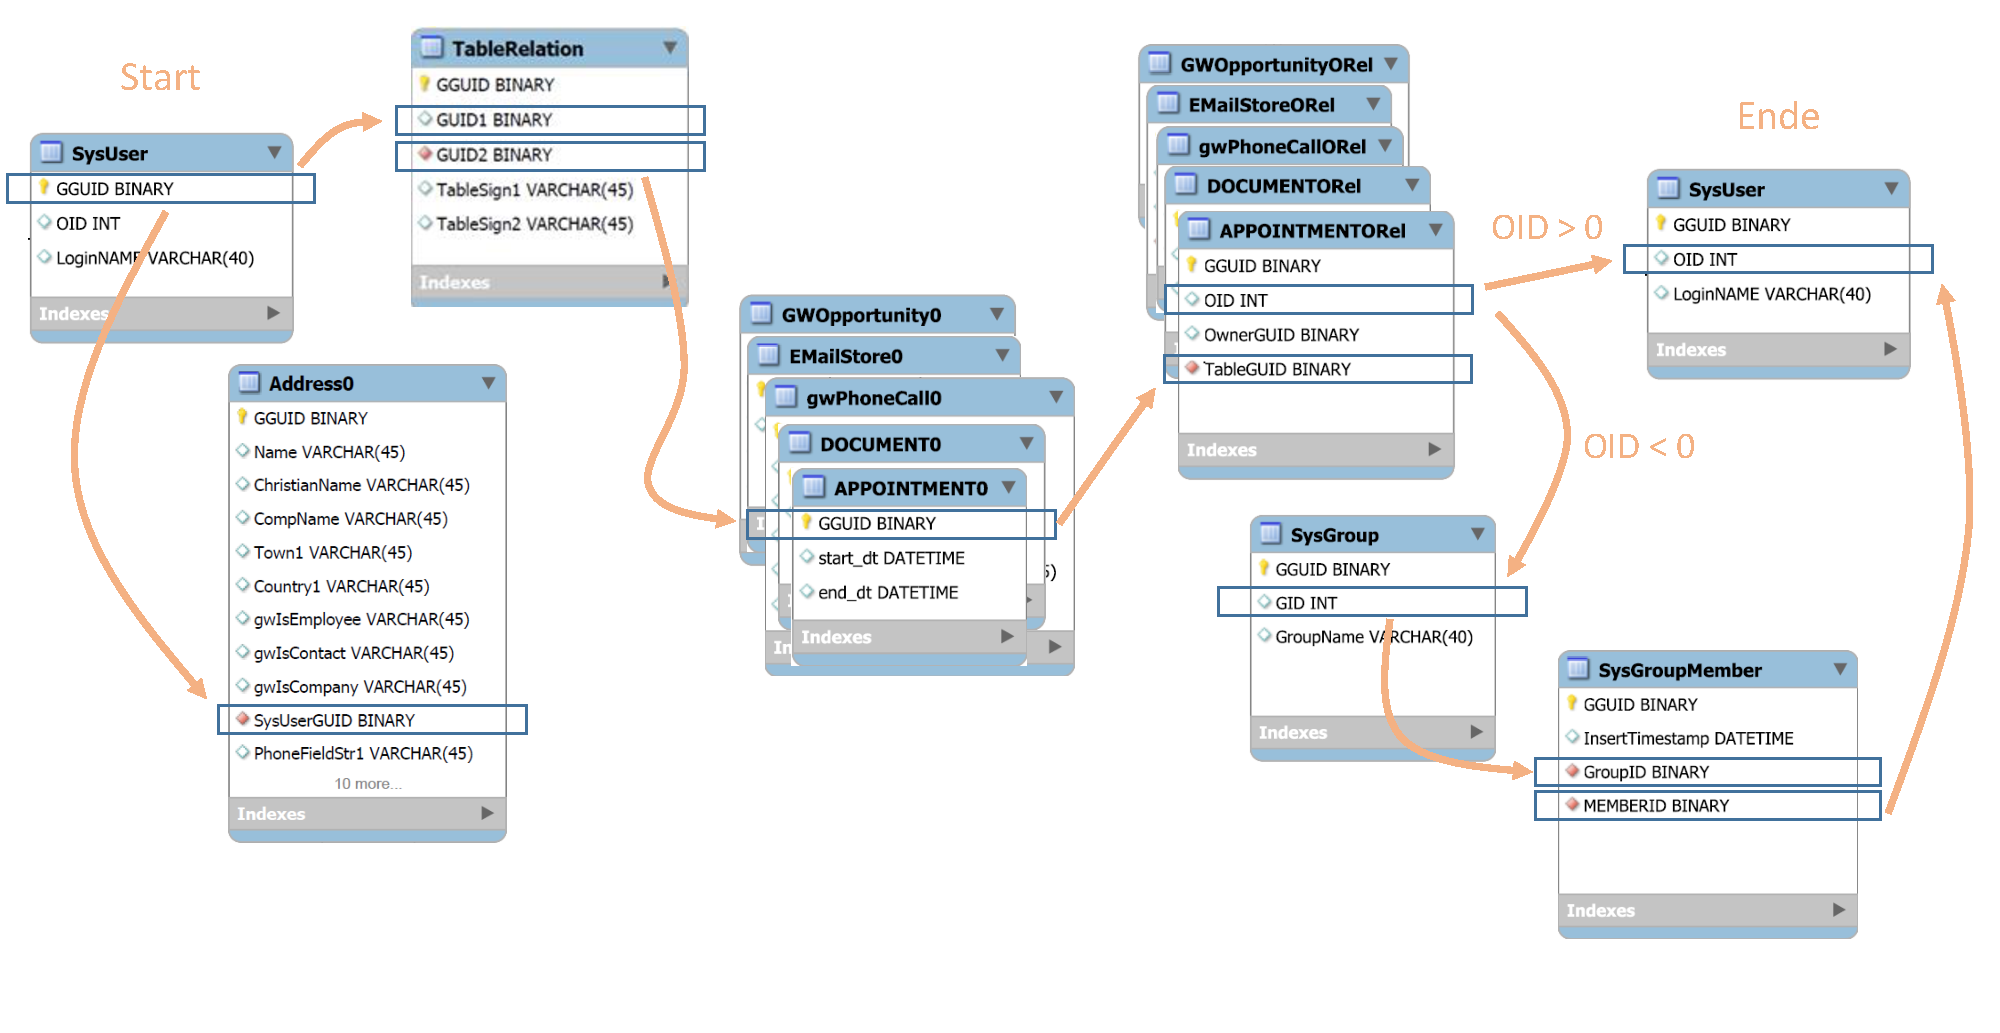
\includegraphics[width=1.0\textwidth]{pics/konzept_extraktion.pdf}
\caption{Vorgehensweise bei der Extraktion}
\label{umsetzung_extract}
\end{figure} 

Mithilfe eines Verbundes zwischen den Tabellen \textit{SysUser} und \textit{Address0} werden die Adressen zu den Personen ermittelt. Anschließend werden durch einen Verbund zwischen \textit{TableRelation} und \textit{SysUser} alle Tabellen ermittelt, mit denen die Personen eine Verknüpfung besitzen. Der nächste Verbund wird zwischen \textit{TableRelation} und einer der fünf zuvor genannten Tabellen gebildet. Um beispielsweise festzustellen mit welchen anderen Personen das Dokument geteilt ist, wird ein weiterer Verbund mit der passenden ORel-Tabelle gebildet. In der ORel-Tabelle kann die \textit{OID} positiv, sowie negativ sein. Bei einem negativen Wert stellt die \textit{OID}, eine \textit{GID} der Tabelle \textit{SysGroup} dar. Zur Auflösung von Gruppen in einzelne Personen werden folgende Verbunde gebildet. Zuerst zwischen \textit{SysGroup} und \textit{SysGroupMember}, um alle Personen die zu einer Gruppe gehören zu erhalten. Anschließend zwischen \textit{SysGroupMember} und \textit{SysUser}, um die \textit{OID} der Person zu erhalten. 

Die durch den Verbund gewonnen Informationen werden weiterhin auf drei relevante Werte verringert. Zu einem die \textit{OID} des \textit{SysUser}, von dem die Suche ausgeht. Zum anderen das Datum, welches durch das CRM-Objekt ermittelt wird. Weiterhin wird die zweite \textit{OID} beibehalten, die durch den Verbund mit einer zweiten \textit{SysUser} Tabelle gewonnen wird. Zum Schluss wird manuell eine vierte Information beigefügt, die besagt welchem CRM-Objekt die Tupel entstammt. 

Für den Sonderfall das ein Datum über mehrere Tage geht, wird eine fünfte Spalte hinzugefügt, welche den Zeitraum in Tagen beinhaltet. Zur Beschaffung der geschobenen Termine wird genau wie in der Konzeption beschrieben verfahren.

Zur Ermittlung von direkten Verbindungen zwischen Personen wird lediglich ein Verbund aus den ORel-Tabellen eines CRM-Objektes gebildet. Dieser Verbund beinhaltet bereits die \textit{OID} der beiden Personen. Zur Ermittlung des Datums wird noch ein Verbund mit der Tabelle des CRM-Objekts gebildet. Die negativen \textit{OID} Werte werden genauso wie oben beschrieben aufgelöst. 

Jedes Ergebnis einer Extraktionsabfrage wird in einer CSV-Datei direkt auf dem Tomcat gespeichert. Diese CSV-Dateien stellen die Grundlage der Transformation dar. Jede dieser Dateien beinhaltet die Werte für die Tabelle \textit{Data} aus der H2-Datenbank, in der Form wie sie in Abbildung \ref{fig:umsetzung_csv_datei} zu sehen ist. 

\begin{figure}[htbp]
\begin{center}
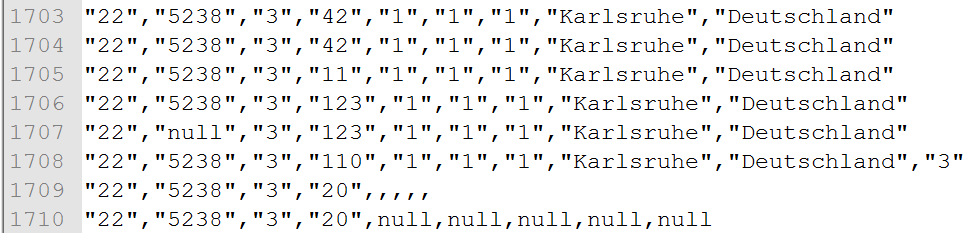
\includegraphics[width=1.0\textwidth]{pics/umsetzung_csv_datei.png}
\caption{Ausschnitt einer CSV-Datei nach der Extraktion}
\label{fig:umsetzung_csv_datei}
\end{center}
\end{figure}

Alle CSV-Dateien werden auf die in Abbildung \ref{fig:umsetzung_csv_datei} zu sehenden Ungereimtheiten untersucht. Dabei wird in Zeilen in denen die letzten fünf Werte fehlen, die Adresse über die \textit{OID} (die vierte Zahl) ergänzt. Bei Nullwerten wird überprüft ob wirklich keine Adresse vorhanden ist, falls doch werden die Adressen ergänzt. Wenn wie in Zeile 1707 zu sehen, ein Nullwert anstatt eines Datum existiert, wird die Zeile entfernt. Wenn wie in Zeile 1708 ein zusätzlicher Wert vorhanden ist, erstreckt sich das Merkmal über mehrere Tage. Die Zeile bleibt bestehen allerdings wird der letzte Wert entfernt. Die Zahl wird jedoch zwischengespeichert, um die entsprechende Anzahl an Tupeln zu erzeugen. Jede dieser Tupeln weist auf einen anderen Tag in der Zeitspanne hin. Nach der Beseitigung von Anomalien werden noch die Städte und Länder durch ihre jeweilige \textit{ID} aus der Tabelle \textit{Town} und \textit{Country} ersetzt.

Die veränderten Daten werden wieder in CSV-Dateien abgelegt. Diese besitzen den gleichen Namen, besitzen allerdings noch den Zusatz "\_transf", der sie als transformiert kennzeichnet. Diese Dateien werden anschließend in einer CSV-Datei zusammengeführt. Bei der Zusammenführung sind zum ersten mal alle Daten gleichzeitig in der Anwendung vorhanden, weshalb an dieser Stelle alle Duplikate beseitigt werden. Weiterhin werden überdies die Zeilen sortiert. Dabei wird mit zwei Kriterien verfahren. Das erste Kriterium ist die \textit{OID} der Person von der die Suche ausgeht. Falls Werte sich gleichen wird das zweite Feld (Datum) herangezogen. Nachdem alle Zeilen sortiert und von Duplikaten bereinigt sind, werden sie in einer CSV-Datei abgelegt. 

Diese Datei werden bei jedem Start der Datenbank verwendet, um einen Bulk-Load für die H2-Datenbank zu initialisieren. Nach dem Einfügen der Daten in die Datenbank werden die Indizes auf den Datensätzen erzeugt.


%% ===========================
\section{Aktualisierung des Datenbestandes}
%% ===========================

Wie zuvor in Abschnitt \ref{ch:Konzeption:sec:updatedatenbestand} behandelt, wird die Aktualisierung unseres Datenbestandes von CAS genesisWorld angestoßen. Die Implementierung ist in Form einer COM-Komponente umgesetzt. Sie wird in einer DLL-Datei definiert. Diese muss Namenskonventionen einhalten. Es werden nur Dateien vom CAS genesisWorld Anwendungsserver erkannt die mit dem Prefix \textit{pGSAxExtCustomServerDataPlugin} beginnen. Die DLL-Datei ist in der \textit{RegisterSDKDataPlugIns.xml} hinterlegt, damit der Anwendungsserver beim Start das Plugin findet. Weiterhin ist in der XML-Datei eine Tabelle paarweise mit einer DLL angegeben. Dadurch wird ein Plugin auf eine Datenbanktabelle registriert und bekommt alle betreffenden Änderungen mit.

Die Programmbibliothek selbst ist in Delphi geschrieben. Abbildung \ref{ergebniss_plugin_klassendiagramm} zeigt die Struktur der DLL-Datei. Die Klasse selbst implementiert sechs verschiedene Schnittstellen. \textit{ComObj} stellt Funktionen zur Erstellung und Bearbeitung von COM-Objekten zur Verfügung. Um Funktionalitäten von CAS genesisWorld vollständig zu nutzen, wird die \textit{ActiveX} Schnittstelle benötigt. Wie bereits behandelt findet die Übertragung der Daten über das REST-Protokoll statt, wofür die \textit{idHttp} Schnittstelle verwendet wird. Um Konvertierungen der vom Anwendungsserver erhaltenen Binärwerte vorzunehmen, werden die Funktionen der Schnittstellen \textit{CAS\_ToolsCOM} und \textit{CAS\_VarType14Fix} genutzt. Das Abfangen der geänderten Daten, welches die eigentliche Kernfunktionalität darstellt, wird durch die Funktionen der \textit{IGWSDKDataPlugin} Schnittstelle implementiert.

Die Funktionen der Abbildung \ref{ergebniss_plugin_klassendiagramm} gehören von \textit{BeforeAddNew()} bis \textit{AfterUndelete()} zur \textit{IGWSDKDataPlugin} Schnittstelle. Es sind zwar alle Funktionen der \textit{IGWSDKDataPlugin} Schnittstelle in der DLL implementiert, allerdings sind nur die Funktionen die mit \textit{After} beginnen auch mit Logik hinterlegt. Für unser System reicht es nämlich aus, über Änderungen im Nachhinein benachrichtigt zu werden. Die Funktionen enthalten alle die gleiche Logik und unterscheiden sich lediglich in den Übergabeparameter.

\begin{figure}[htbp]
\centering
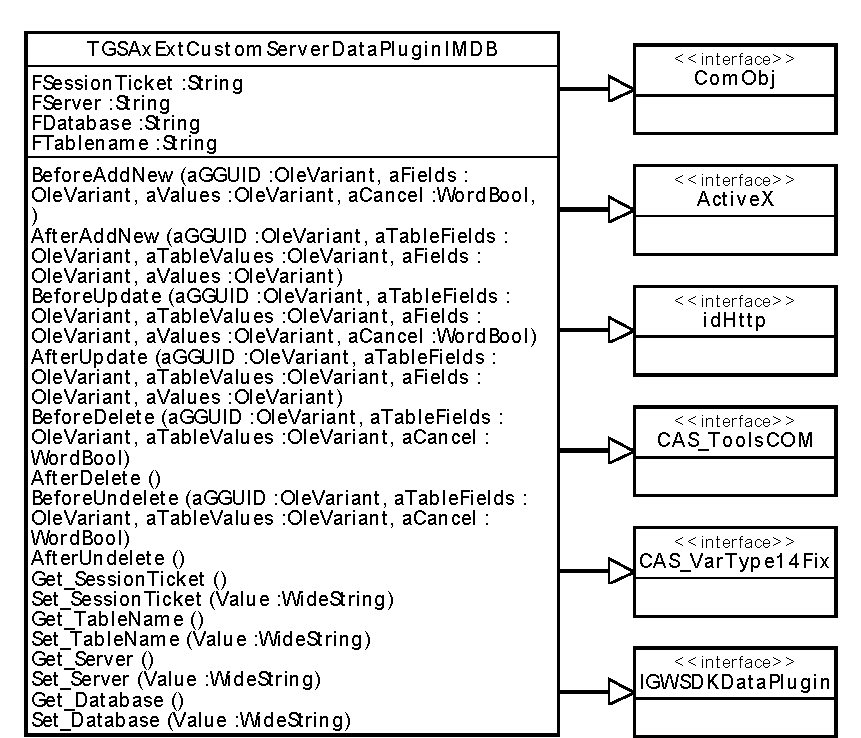
\includegraphics[scale=0.7]{pics/plugin_klassendiagramm.pdf}
\caption{Klassendiagramm Plugin}
\label{ergebniss_plugin_klassendiagramm}
\end{figure}

Die Funktionsweise wird im Folgenden anhand der Abläufe in der Logik erläutert und sind auch in der Abbildung \ref{konzept_sequenz} zu sehen. Nachdem der Benutzer Datensätze geändert hat wird das Plugin aufgerufen. Die entsprechende Funktion erhält die \textit{GGUID} der Tupel, den Namen der Spalte, sowie die veränderten Werte. Anschließend wird überprüft, ob die Änderungen für unser System von Relevanz ist. Falls sie sich als relevant herausstellen, wird die \textit{aGGUID} in einen String konvertiert. Anschließend werden die Header-Werte der \textit{idHttp} Variable gesetzt. Sie beinhalten Werte wie die URI oder HTTP-Metadaten. Sobald alle Daten in der \textit{idHttp} gesetzt sind, wird ein POST-Request an unser System übermittelt. 

Der POST-Request enthält lediglich die \textit{GGUID} und die Art der Operation, die auf den Daten ausgeführt wurde. Bei neuen Daten beispielsweise wird ein Header namens "newGGUID" und dem Wert der \textit{GGUID} gesetzt. Im Anwendungsserver wird der neue Wert zuerst in eine CSV-Datei geschrieben und anschließend in die Datenbank eingefügt.


\begin{figure}[htbp]
\centering
  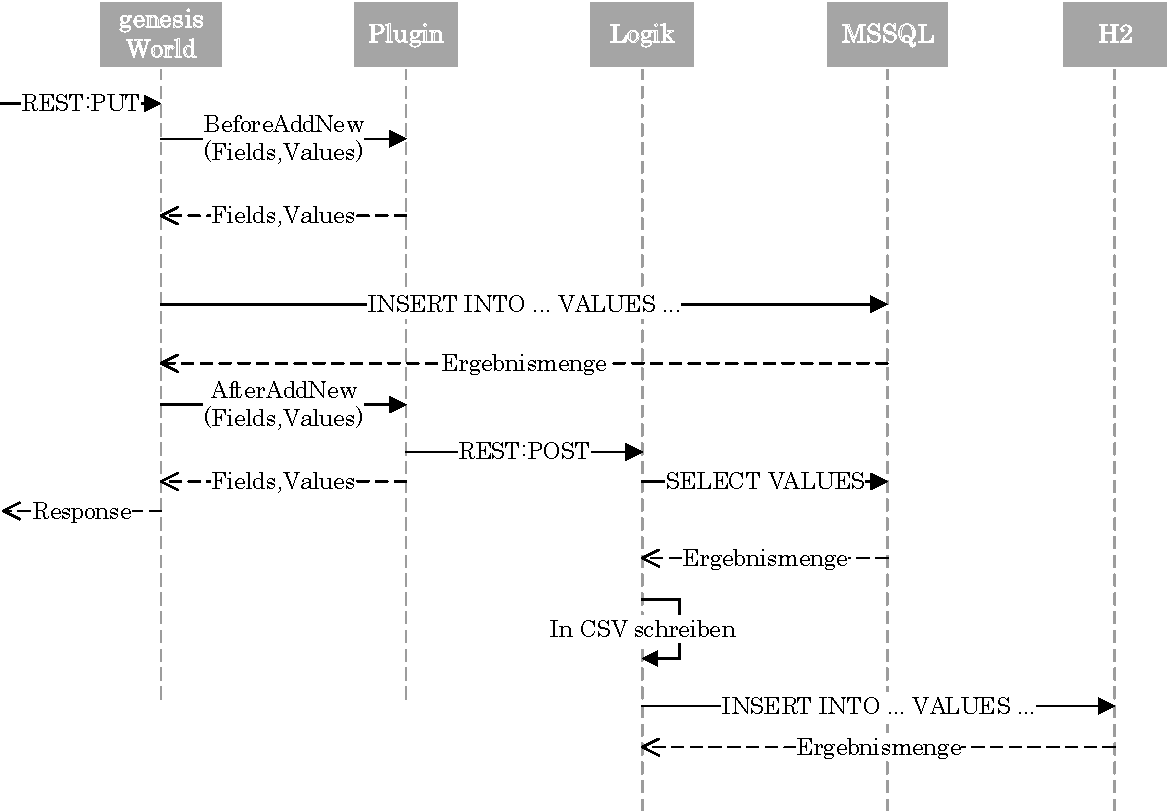
\includegraphics[width=0.8\textwidth]{pics/sequenzdiagramm.pdf}
\caption{Sequenzdiagramm für einen neuen Datensatz}
\label{konzept_sequenz}
\end{figure}



%% ===========================
\section{Oberfläche}
%% ===========================

In diesem Abschnitt wird die Umsetzung der Darstellung erörtert. Den Einstiegspunkt für Nutzer stellt das in Abbildung \ref{ergebniss_oberflaeche_anmeld} zu sehende Anmeldefenster dar. Der Hintergrund der Webseite ist in einem dunklen grau gestaltet, um einen Kontrast zum weißen Hintergrund der Bedienelemente zu schaffen. Dadurch werden die für den Nutzer verwendbaren Bereiche abgehoben. Zur Identifikation des Systems mit der Firma ist das Logo der CAS Software AG im linken Teil abgebildet. Im rechten Teil des Fensters existieren drei Eingabefelder. Zuerst ein Feld zur Eingabe der IP-Adresse des Server. Die dazugehörige Portnummer wird im darauf folgenden Feld eingegeben. Das dritte Feld ist für den Namen des Nutzers vorgesehen, der den Ausgangspunkt der Analyse darstellt. Abschließend wird ganz klassisch ein Button zum fortfahren auf der Webseite eingesetzt. Falls allerdings der eingegeben Nutzername nicht existiert, wird eine Warnmeldung direkt über dem zweiten Eingabefeld ausgegeben. 

\begin{figure}[htbp]
\centering
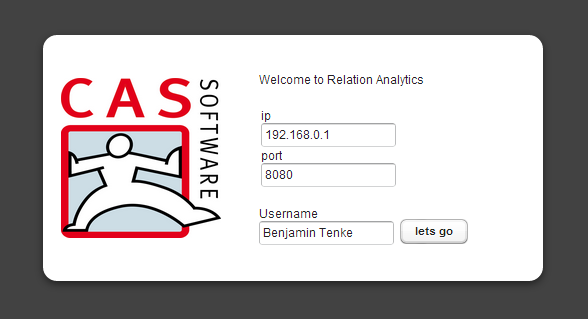
\includegraphics[scale=2.0]{pics/login.png}
\caption{Anmeldefenster}
\label{ergebniss_oberflaeche_anmeld}
\end{figure}

Das Hauptfenster wurde vom Aufbau, wie in Abschnitt \ref{ch:Konzeption:sec:Darstellungskonzepte} beschrieben umgesetzt. Im oberen Bereich befindet sich eine Leiste, die anhand der Microsoft Richtlinien für Design entworfen wurde. Dies schafft ein vertrautes Gefühl mit der Oberfläche und schafft eine schnelle Akzeptanz bei den Nutzern. Die Leiste ist in vier Bereiche aufgeteilt. Der erste Bereich, ganz links, dient der Gewichtung der Verbindungsmerkmale und dem anstoßen der Abfrage. Aufgrund der Gewichtung in Prozent, ist ein fester Wertebereich von 0 bis 100 vorgegeben. Textfelder eignen sich daher weniger, da sie beliebige Eingaben ermöglichen. Der Einsatz von Reglern bietet eine einfachere und selbsterklärende Form der Bedienung. Der begrenzte und kleine Wertebereich begünstigen den Einsatz der Regler. Zum stellen der Anfrage wird ein einfacher Button eingesetzt. Direkt unter dem Button befindet sich ein Text, der die benötigten Zeit für die Abfrage ausgibt. 

Der zweite Bereich dient zeitlichen Anpassungen. Das erste und dritte Feld können für Veränderung des Betrachtungszeitraums verwendet werden. Sie beinhalten den Anfangs- und Endzeitpunkt. Händische Eingaben weisen eine schlechte Bedienbarkeit auf, weswegen ein sogenannter "Datumspicker" eingesetzt wird. Dieser befindet sich direkt neben dem Textfeld und öffnet sich nach einem Klick auf das Symbol. Er stellt einen grafischen Kalender dar, aus dem durch klicken auf ein Tag das Datum bestimmt werden kann. Die Möglichkeit zur Eingabe durch direktes ändern des Textes bleibt allerdings weiterhin erhalten. Die anderen beiden Felder sind für die Gewichtung der Zeit vorgesehen. Diese Felder dienen zur Festlegung von $t_1$ und $t_2$, aus der Abbildung \ref{fig:umsetzung:gewichtungderzeit}. Das obere Feld ist für $t_1$. Hier kann die Zeitspanne zwischen $t_{s}$ und $t_1$ in Tagen festgelegt werden. Für $t_{e}$ und $t_2$ verhehlt es sich wie mit dem unteren Feld.

Bis auf die Gruppenfilterung sind im dritten Bereich alle restlichen Filtermöglichkeiten vorhanden. Mithilfe von Checkboxen kann der Nutzer festlegen, welche Filterungen auf die Analyse angewendet werden sollten. Neben der Filterung durch bestimmte Personen, Länder, Städte usw. ist hier eine Begrenzung der Ergebnismenge umgesetzt. Im untersten Feld kann der Nutzer diese bestimmen.

Der Bereich ganz rechts in der Leiste, ist für den Ausschluss von Gruppen vorgesehen. Hier werden alle Gruppen im System mit einer Checkbox und einem Namen dargestellt. Dabei können beliebig viele Gruppen ausgewählt werden. Da die Anzahl der Gruppen überschaubar ist, entschied man sich alle anzuzeigen, anstatt einer händischen Eingabe der Namen durch den Nutzer. Für Benutzer entsteht dadurch ein Vorteil, da sie Gruppen auswählen können die sie zuvor nicht kannten.

\begin{figure}[htbp]
\centering
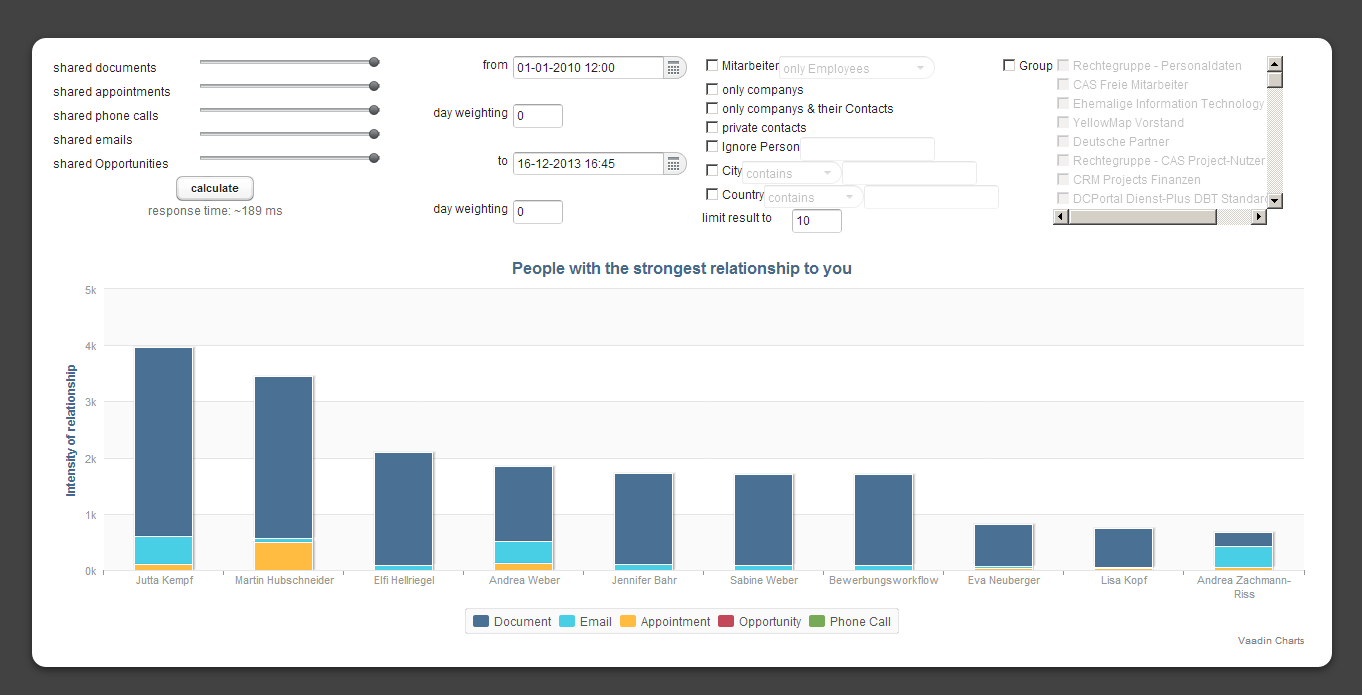
\includegraphics[width=\textwidth]{pics/final_screen.png}
\caption{Hauptseite der Anwendung}
\label{ergebniss_oberflaeche_haupt}
\end{figure}

Den zentralen Bereich des Fensters stellt das Diagramm dar. Die Balken selbst sind in fünf verschiedene Elemente unterteilt. Jedes Elemente wird dabei, durch eine andere Farbe dargestellt. Die fünf Elemente sind die verschiedenen Verbindungsmerkmale. Die Zuordnung der Farbe zu dem jeweiligen Merkmal, wird über eine Legende im unteren Bereich des Fensters umgesetzt. Eine Besonderheit ist, dass durch einen Klick auf eine der Farben, das jeweilige Merkmal von der Darstellung ausgeschlossen wird. Beispielsweise kann der Nutzer auf die blaue Farbe neben dem Dokument klicken, was einen Neuaufbau des Diagramms ohne Dokumente bewirkt. Durch den Ausschluss wird allerdings keine neue Abfrage gesendet. Das  bedeutet die Reihenfolge in der die Personen angezeigt werden die Datenbasis gleich  bleiben. Mit einem wiederholten Klick lässt sich der Originalzustand wiederherstellen. Zusätzlich zu der y-Achse, die eine Gesamtpunktzahl aufzeigt, kann der jeweilige Anteil eines Merkmals betrachtet werden. Dies geschieht durch einfaches platzieren des Mauszeigers, auf dem jeweiligen Bereich des Balkens. Dadurch öffnet sich ein Tooltip, welches die Anzahl der Punkte im Verhältnis zur Gesamtpunktzahl zeigt.

Die Ausführung der Anfrage erfolgt in der Regel mit dem dafür vorgesehen Button. Die Regler und das Datum, jedoch lösen bei Veränderungen automatisch eine neue Abfrage aus. Dies soll die hohe Antwortgeschwindigkeit des Systems untermalen und eine bessere Nutzererfahrung schaffen. Das Datum, sowie die Gewichtung wurden dazu ausgewählt, da sie die am meisten benutze Konfigurationsmöglichkeit darstellen.


%% Cahpter_Zusammenfassung.tex
%%

%% ===========================
\chapter{Fazit und Ausblick}
\label{ch:Ergebnis}
%% ===========================

In diesem abschließenden Kapitel werden die Ergebnisse der Arbeit in ihren wichtigsten Punkten zusammengefasst und anhand der Anforderungen aus Kapitel \ref{ch:Systemanalyse:sec:Anforderungsanalyse} bewertet. Anschließend wird ein Ausblick auf weiterführende Möglichkeiten, sowie zukünftige Verbesserungsmöglichkeiten gegeben. 

%% ===========================
\section{Zusammenfassung}
\label{ch:Ergebnis:sec:zusammenfassung}
%% ===========================

Aus der Motivation heraus wurde in der vorliegenden Arbeit ein System, basierend auf den Daten von CASgenesisWorld entwickelt. Hierzu wurden zuerst alle relevanten Komponenten von CASgenesisWorld untersucht. Dabei wurden Tabellen und Spalten identifiziert, die zur Realisierung der Lösung notwendig sind. Anschließend wurden die Anforderungen an das neue System erhoben. Mit dem Wissen über die zu übernehmenden Daten und den Anforderungen wurde eine passende Datenbank ausgewählt. Diese sollte den zuvor erhobenen Anforderungen gerecht werden. Dabei wurden NoSQL-Datenbanken hinsichtlich ihrer Eignung untersucht. Sie konnten in diesem Fall allerdings nicht überzeugen, somit entschied man sich für die H2-Datenbank. Die Entscheidung zugunsten der H2-Datenbank ist auf die im Hauptspeicher gehaltenen Tabellen zurückzuführen.   

Aufbauend auf der zuvor ausgewählten Datenbank wurden Konzepte zur Umsetzung des Systems entwickelt. Bei der Konzeption wurde deduktiv vorgegangen. Zuerst wurde die Architektur definiert und anschließend die einzelnen Komponenten detailliert geplant. Bei der Planung wurde nicht versucht ein universell einsetzbares System zu entwickeln, sondern vielmehr eine domänenspezifische Lösung für das Szenario auszuarbeiten. Nachdem alle Technologien, sowie Vorgehensweisen festgelegt wurden, ging man auf die Umsetzungen ein. Indessen eine Beschreibung der Funktionsweise einzelner Komponenten durchgeführt wurde. Neben der Funktionsweise wurde die Interaktion unter den Komponenten dargelegt. Schlussendlich wurde die fertige Oberfläche und die getroffenen Designentscheidungen dargelegt.
 
%% ===========================
\section{Bewertung der Ergebnisse}
\label{ch:Ergebnis:sec:bewertung}
%% ===========================

Die funktionalen Anforderungen konnten alle umgesetzt werden und wurden bereits im vorherigen Kapitel anhand der Oberfläche erläutert. Im folgenden wird somit auf die Erfüllung der nicht funktionalen Anforderungen eingegangen. Dies erfolgt anhand der Gegenüberstellung von Anforderungen und den Charakteristika des Systems.

Die erste Anforderung konnte durch den Betrieb auf einem Server eingehalten werden. Weiterhin wurde eine lose Kopplung erreicht. Diese spiegeln sich in den REST-Schnittstellen der jeweiligen Komponenten wieder. Überdies gibt es keine Abhängigkeiten zwischen den Klassen der Darstellung und den Klassen der Geschäftslogik. Ein gewisses Maß an Portabilität wurde vorausgesetzt, damit ein verlagern des Systems auf andere Instanzen kein Problem darstellt. Dies wurde durch die Verwendung der Web-Archive-Dateien erreicht. Sie ermöglichen den Einsatz auf verschiedenen Tomcat Servern, was sie nicht nur portabel macht, sondern auch verschiedenen Servern einsetzbar macht. 

Einer der wichtigsten Anforderungen ist die geringe Abfragegeschwindigkeit. Tabelle \ref{tb:vergleichAbfragegeschwindigkeit} zeigt, dass man dieser Forderung gerecht wird. Ebenfalls deutlich zu erkennen ist die Auswirkung des geänderten Schemas. Der Sprung von 98.000 ms auf 350 ms ist durch die Reduktion in der Abfragekomplexität zu erklären. Die Abfragen erfolgen über wesentlich weniger Tabellen und Spalten als zuvor. Außerdem wird im neuen Schema kein Verbund in der Datenbankabfrage mehr benötigt. Allerdings sind bei derartigen Maßnahmen, wie sie im Schemadesign ergriffen wurden, weitreichende Folgen zu beachten. Eine davon ist eine sehr schlechte Erweiterbarkeit des Schemas. Im momentanen Schema können lediglich Spalten hinzugezogen werden, dessen Inhalt in allen Verbindungsmerkmalen vorhanden ist. Außerdem würden für jede weitere Spalte, 18 Mio. zusätzliche Werte entstehen. Die Hinzunahme von merkmalspezifischen Attributen würde ebenfalls zu hohen Änderungsaufwänden führen. Als eine Konsequenzen müsste die \textit{data} Tabelle in mehrere Tabellen aufgeteilt werden. Dies würde eine stärke Normalisierung des Schemas bewirken und den Einsatz von Verbundoperatoren erfordern. Dadurch würde die Verarbeitungsgeschwindigkeit bei Lesezugriffen steigen. Allerdings wären dennoch wesentlich weniger Verbundoperatoren als im alten Schema nötig. Aufgrund dessen ist trotzdem mit einer deutlichen geringeren Abfragegeschwindigkeit als in CASgenesisWorld zu rechnen.  

\begin{table}[htbp]
\centering
\begin{tabular} {l | r}
Versuchskomponente & Zeit in ms  \\ \hline
MSSQL Datenbank \& Altes Schema & 98000 \\
MSSQL Datenbank \& Neues Schema & 350 \\
H2 Datenbank \& Neues Schema & 80 \\
\end{tabular}
\caption{Abfragegeschwindigkeit Vergleich}
\label{tb:vergleichAbfragegeschwindigkeit}
\end{table}

Nachdem Änderungen welche eine Steigerung der Komplexität bewirken betrachtet wurden, stellt sich folgende Frage: Ist die Datenbank nur aufgrund des geänderten Schemas deutlich schneller? Um dieser Frage nachzugehen wurden Tests durchgeführt. Abbildung \ref{ergebniss_vergleich} zeigt die Ergebnisse dieser Testreihen. Alle Testläufe wurden auf einem Client durchgeführt. Dieser simulierte mithilfe von Multithreading den Zugriff von 100 gleichzeitigen Benutzern. Die in den Diagrammen angegebene Zeit bezieht sich somit auf die Ausführung aller 100 Abfragen. Jeder simulierte Benutzer führt die auf der y Achse angegebene Anweisung aus. Beim obersten Balken in (a) sind es beispielsweise 15 Mio. SELECT-Anweisungen pro Benutzer. In (b) hingegen wird die Verarbeitungsgeschwindigkeit bei Updates verglichen. Der Vergleich anhand von Insert-Anweisungen wird in (c] gezeigt.    

\begin{figure}[htbp]
\centering
\subfigure[Vergleich anhand Select-Performance]{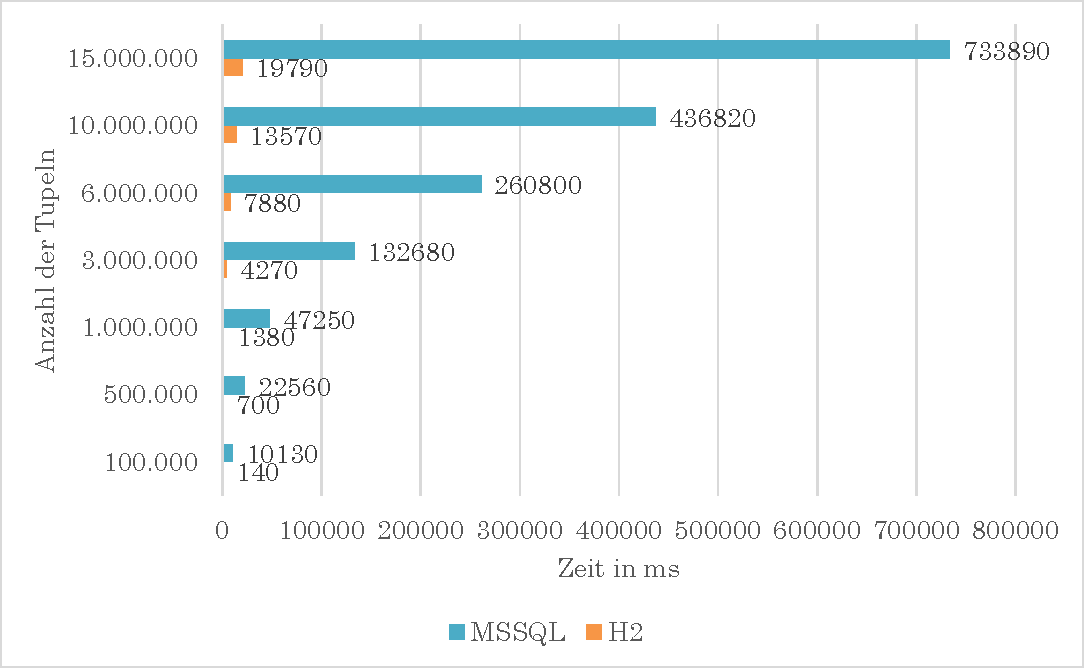
\includegraphics[width=0.49\textwidth]{charts/select.pdf}}\hfill
\subfigure[Vergleich anhand Update-Performance]{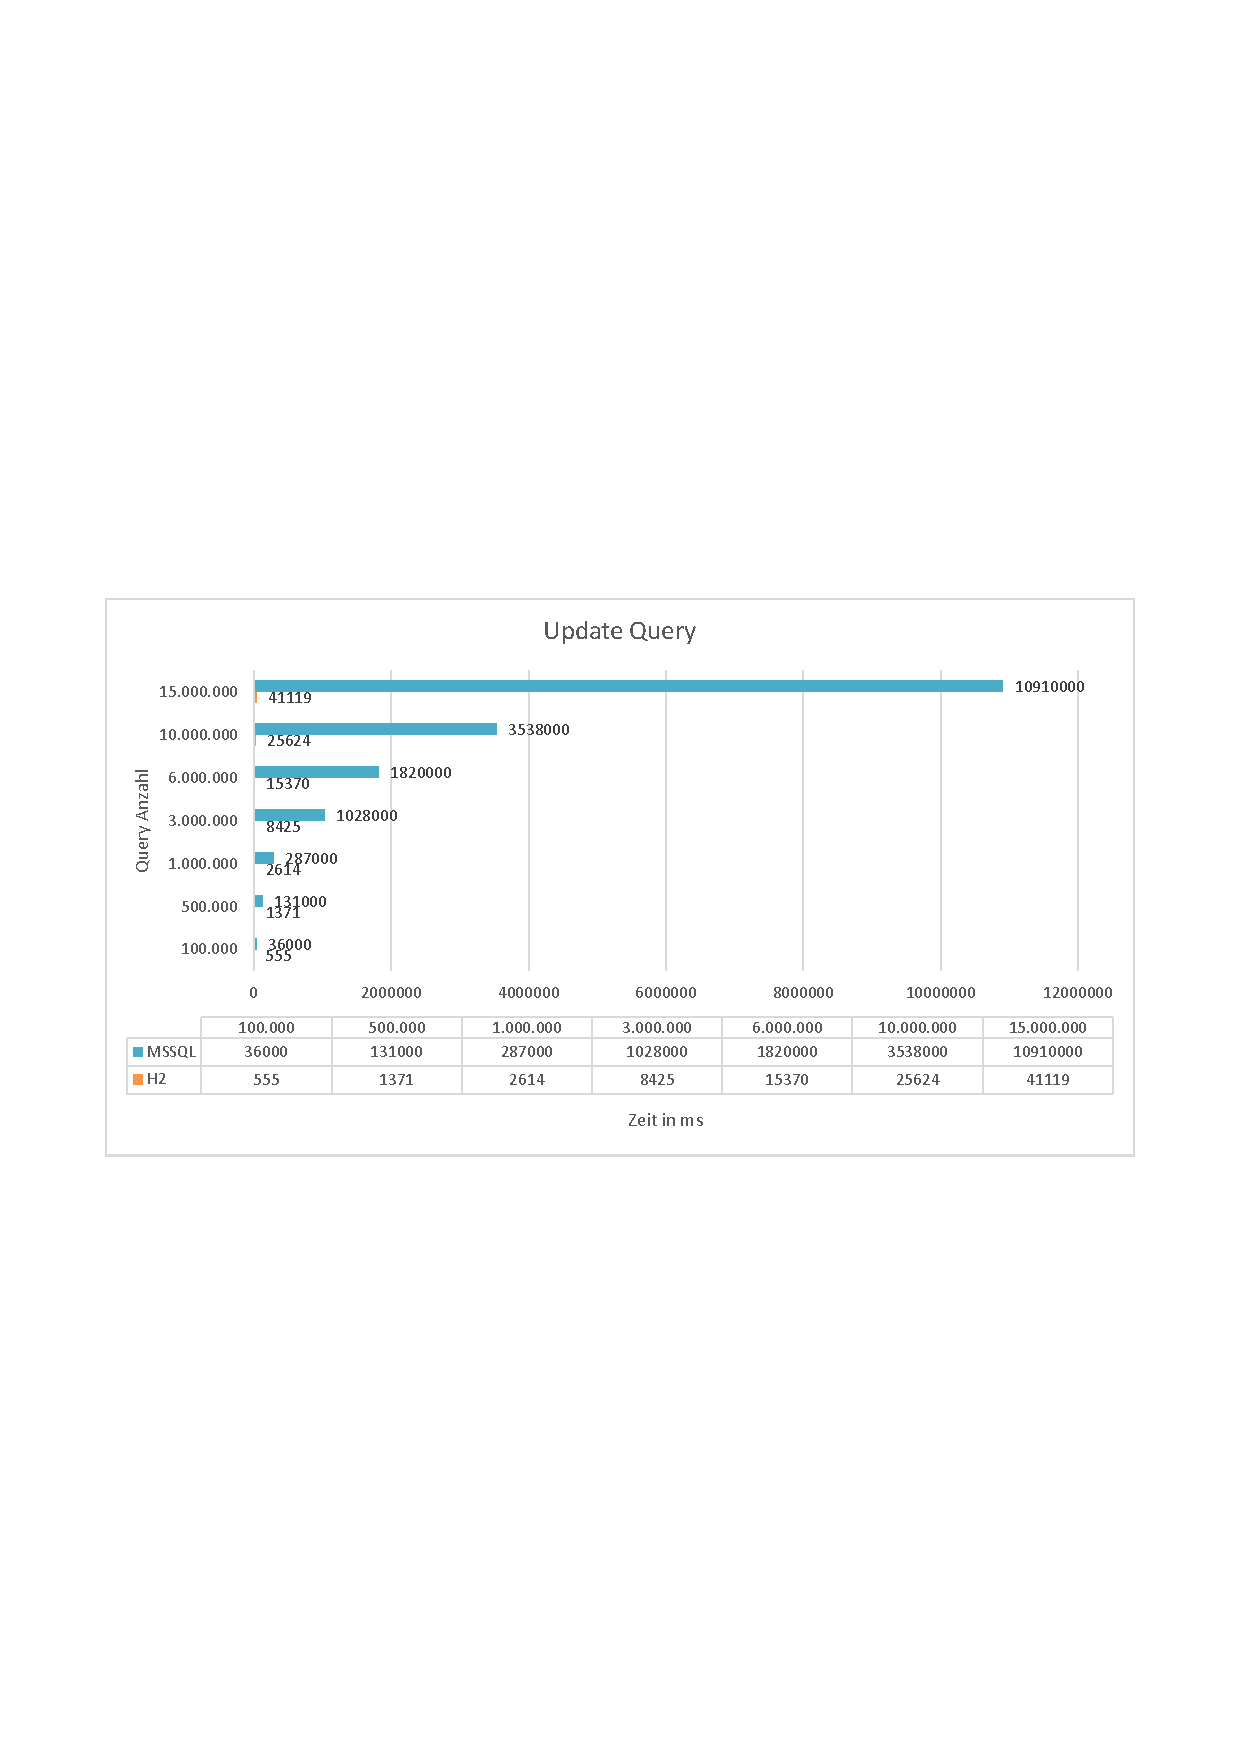
\includegraphics[width=0.49\textwidth]{charts/update.pdf}}\hfill
\subfigure[Vergleich anhand Insert-Performance]{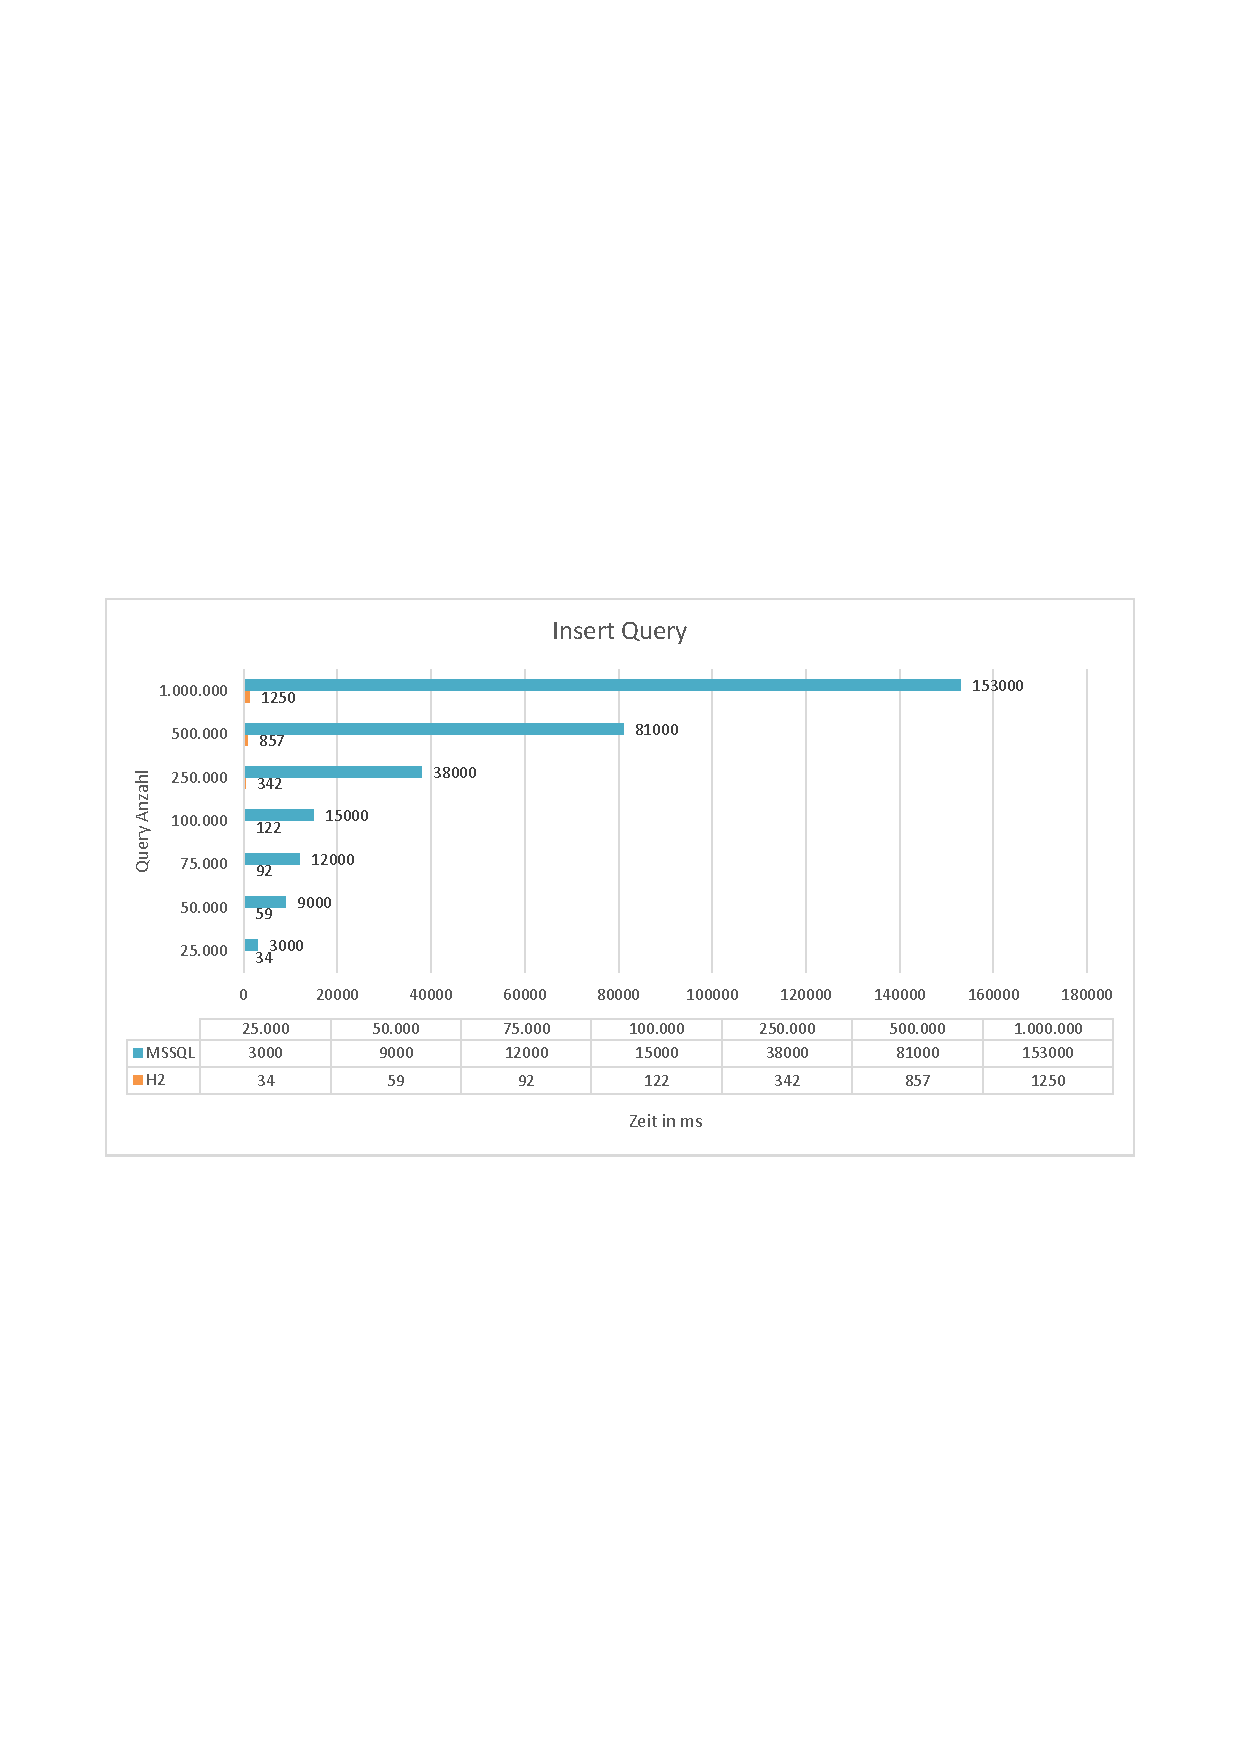
\includegraphics[width=0.5\textwidth]{charts/insert.pdf}}
\caption{Abfragegeschwindigkeit Vergleich}
\label{ergebniss_vergleich}
\end{figure}

Die Ergebnisse der Tests zeigen, dass die H2-Datenbank bei den durchgeführten Tests deutlich schneller als die MSSQL Datenbank ist. Der H2 ist bei SELECT-Anweisungen, um den Faktor 37 schneller. Bei Update-Anweisungen sogar um den Faktor 117. Ebenso bei Insert-Anweisungen, die einen Unterschied um den Faktor 124 aufweisen. Daraus lässt sich ableiten, dass die H2-Datenbank durch ihre In-Memory-Tabellen deutlich an Geschwindigkeit, im Gegensatz zu herkömmlichen Datenbanken, gewinnt. Diese Geschwindigkeit wird zum Teil durch den Verzicht auf Persistenz erlangt. Würde die Datenbank ihre Daten zur Sicherung auf die Festplatte schreiben, müsste bei Schreiboperationen mit Performance-Verschlechterungen gerechnet werden. Im vorliegenden System, welches fast nur Leseoperationen durchführt, stellt die mangelnde Persistenz allerdings kein großes Defizit dar. Ausschlaggebend für die Schnelligkeit ist allerdings die Nutzung des Hauptspeichers als Speichermedium. Dessen Gebrauch könnte allerdings in der Zukunft aufgrund der immer größer werdenden Datenmengen ein Problem darstellen.  

%% ===========================
\section{Ausblick}
\label{ch:Ergebnis:sec:Ausblick}
%% ===========================

Mit der Umsetzung des in der Arbeit beschriebenen Systems steht eine eine performante Lösung bereit, die eine Bewertung der Ausprägung von Beziehungen zwischen Personen aus einem CRM-System ermöglicht.

Die Bewertung der Beziehungen beruht derzeit lediglich auf der Anzahl von Verbindungsmerkmalen. Dementsprechend wird nur die Häufigkeit gewertet. Um die Bewertung einer Beziehungsausprägung genauer feststellen zu können, werden zusätzliche Regeln benötigt. Diese Regeln sollten auf psychologischen Erkenntnissen und Erfahrungswerten aufbauen. Durch Regeln ließe sich die Aussagekraft von Ergebnissen weiter steigern. Beispielsweise sind kommunikative Kontakte wie Telefonate oder E-Mail Verkehr, kein Indikator für Vertrauen. Die Einsicht in vertrauliche Dokumente setzt dagegen eine engere Zusammenarbeit oder Vertrauen voraus. Dies sollte somit stärker gewichtet werden. 

Neben den festen Regeln sind Vorschläge für die Benutzer über verschiedenen Gewichtung der Verbindungsmerkmale sinnvoll. Dabei kann der Nutzer zwischen verschiedenen Vorgaben wählen, die basierend auf Erkenntnissen und Erfahrungen beruhen. Die Vorgaben würden verschiedene Charakteristiken verkörpert. Eine solche Vorgabe könnte sein: Ermittlung der Ausprägung zu Personen mit denen ich direkten Kontakt habe. In diesem Fall würden Gespräche, E-Mail Verkehr, Termine mit den jeweiligen Personen wesentlich stärker gewertet werden als beispielsweise Dokumente.

Weiterhin kann durch den Einsatz des Systems der Vertrieb eines Unternehmens unterstützt werden. Eines der denkbaren Szenarien setzt eine Erweiterung des Systems voraus. Dazu bräuchte man zusätzliche Informationen über den Wert einer Person für die Firma. Mit diesen Informationen müsste wie bei der Beziehung ein Ranking aufgestellt werden. Nun wäre ein Vergleich der Rankings möglich, anhand dessen starke Diskrepanzen vom Wert einer Person und mit dessen Beziehungsausprägung erkennbar wären. So könnte Verhältnismäßigkeiten im Aufwand und Nutzen entdeckt werden.

Außerdem könnte jeder Vertriebsmitarbeiter mithilfe des Systems individuell unterstützt werden. Beispielsweise könnten Vertriebsmitarbeiter überprüfen, ob sie dem jeweiligen Kunden genug Zeit widmen oder anderen zu wenig. Weiterhin könnte das Ranking durch eine einfache Anpassungen der Abfrage so geändert werden, dass Personen angezeigt werden, dessen Beziehung zu einer Person am niedrigsten ausgeprägt sind. Was wiederum eine Überprüfung auf mangelhafte Kundenpflege ermöglicht. 
Überdies könnten Möglichkeiten zum Vergleich mehrerer Personen realisiert werden. Der Vergleich könnte dabei unter Personen aus einer Gruppe oder aus einer durch den Nutzer zusammengestellten Menge erfolgen. Mithilfe eines Vergleichs unter Vertriebsmitarbeitern könnte überprüft werden, ob die Verteilung der Kunden auf einzelne Mitarbeiter effizient gestaltet ist. Beispielsweise läse sich damit feststellen ob zu viele Mitarbeiter sich unwissentlich auf denselben Kunden konzentrieren.

Eine weitere weiterführende Möglichkeit, wäre die Hinzunahme einer Darstellung über die Entwicklung der Beziehungen über die Zeit hinweg gesehen. Liniendiagramme wären dabei eine geeignete Form der Visualisierung, da sich mit ihnen zeitliche Abläufe gut darstellen lassen. Mithilfe des momentanen Datenbestandes ist dies möglich, es muss lediglich eine Abfrage und die Darstellung dazu implementiert werden.  


%% --------------------
%% |   Bibliography   |
%% --------------------
\cleardoublepage
\phantomsection
\addcontentsline{toc}{chapter}{\bibname}

\iflanguage{english}
{\bibliographystyle{IEEEtranSA}}	% english style
{\bibliographystyle{babalpha-fl}}	% german style
												  
% Use IEEEtran for numeric references
%\bibliographystyle{IEEEtranSA})


\bibliography{thesis}



%% ----------------
%% |   Appendix   |
%% ----------------
\cleardoublepage

%% appendix.tex
%%

%% ==============================
%\chapter{Appendix}
%\label{ch:Appendix}
%% ==============================






\end{document}